\ifdefined\fullversion
\else
\def\fullversion{1}    % 0 = conference version; 1 = full version
\fi

\ifdefined\cameraversion
\else
\def\cameraversion{0}    % 0 = long version; 1 = proceedings version
\fi
\def\showoverflow{1}   % 1 = show overflows
\def\allow{1}      % 0 = remove todo command
\def\anonymous{1}      % 1 = anonymous

% \documentclass[envcountsame,runningheads,notitlepage]{llncs}
\documentclass[envcountsame,runningheads,notitlepage]{llncs}
\ifnum\fullversion=1
\usepackage[a4paper, margin=1.1in]{geometry}
\setlength{\marginparwidth}{2.5cm}
\fi

\usepackage{makecell}
\usepackage{amsmath} 
% \usepackage{amsthm} don't use this, makes errors
% \usepackage{wasysym} don't use this, makes errors
\usepackage[utf8]{inputenc}
\usepackage[T1]{fontenc}
% \usepackage{hyperref}
\usepackage{verbatim}
\usepackage{tikz}
\usetikzlibrary{positioning,calc}
\usepackage{xspace}
\usepackage{amssymb}
\usepackage{mathtools}
\usepackage{pifont}
\usepackage{etoolbox}
% \usepackage[normalem]{ulem}
\usepackage{booktabs}
\usepackage{bookmark}
% \usepackage[bookmarks=true]{hyperref} 
\usepackage{float} %to force my protocol environment to stay where it is

\usepackage{array}
\usepackage[capitalise,noabbrev]{cleveref}
\usepackage{cite}
\usepackage{multibib}
\usepackage{url}
\usepackage{algorithm}
% \usepackage{algpseudocode}
\usepackage{paralist}
\usepackage{mathrsfs}
\usepackage{relsize}
\usepackage{stmaryrd}
\usepackage[textsize=small]{todonotes}
\usepackage{multirow}
% \usepackage[lambda,n,operators]{cryptocode}
% \usepackage{caption} % Removed to avoid warning with llncs class
\usepackage[skip=10pt plus1pt, indent=40pt]{parskip}
\usepackage{cancel} 
\usepackage[
n,
advantage,
operators,
sets,
adversary,
landau,
probability,
notions,
logic,
ff,
mm,
primitives,
events,
complexity,
oracles,
asymptotics,
keys
]{cryptocode}
\createpseudocodeblock{pcb}{center,boxed}{}{}{}

\newtoggle{notes}
\toggletrue{notes} % set to false to remove colored notes from the paper


%--------------------------------------------------------
% Custom - commitment and PS sigs
%--------------------------------------------------------
\newcommand{\BG}{\mathsf{BG}}
\newcommand{\BGGen}{\mathsf{BGGen}}
\newcommand{\Setup}{\mathsf{Setup}}
\newcommand{\OrgKeyGen}{\mathsf{OrgKeyGen}}
\newcommand{\UserKeyGen}{\mathsf{UserKeyGen}}
\newcommand{\Obtain}{\mathsf{Obtain}}
\newcommand{\Issue}{\mathsf{Issue}}
\newcommand{\MIMCABC}{\ensuremath{\mathsf{MIMC\text{-}ABC}}\xspace}
\newcommand{\UNF}{\ensuremath{\mathsf{UNF}}\xspace}
\newcommand{\UNFONE}{\ensuremath{\mathsf{UNF\text{-}1}}\xspace}
\newcommand{\UNFTWO}{\ensuremath{\mathsf{UNF\text{-}2}}\xspace}


\newcommand{\Nul}{\mathsf{N}}
\newcommand{\nul}{\mathsf{N}}
\renewcommand{\exp}{\mathsf{exp}}
\newcommand{\n}{\mathsf{n}}
\newcommand{\ABC}{\mathsf{ABC}}



\newcommand{\acu}{\mathsf{ACU}}
\newcommand{\acusetup}{\mathsf{ACU.Setup}}
\newcommand{\acuadd}{\mathsf{ACU.Add}}
\newcommand{\acudel}{\mathsf{ACU.Del}}
\newcommand{\acuvermem}{\mathsf{ACU.VerMem}}
\newcommand{\acuvernonmem}{\mathsf{ACU.VerNonMem}}


\newcommand{\rev}{\mathsf{REV}}
\newcommand{\revsetup}{\mathsf{REV.Setup}}
\newcommand{\revrevoke}{\mathsf{REV.Revoke}}
\newcommand{\revtokengen}{\mathsf{REV.TokenGen}}
\newcommand{\revtokenver}{\mathsf{REV.TokenVer}}

\newcommand{\rt}{\mathsf{rt}}

% \newcommand{\tilcm}{\tilde{\mathsf{cm}}}
\newcommand{\tilcm}{\tilde{cm}}


\renewcommand{\k}{\mathsf{k}}
\newcommand{\mb}{\textbf{m}}
\newcommand{\gb}{\textbf{g}}
\newcommand{\tilgb}{\tilde{\textbf{g}}}
\newcommand{\yb}{\textbf{y}}
\newcommand{\rd}{\Delta_r}
\newcommand{\td}{\Delta_t}
\newcommand{\ud}{\Delta_u}


%--------------------------------------------------------
% Custom - Syntax
%--------------------------------------------------------

\renewcommand{\st}{\mathsf{st}}
\newcommand{\zkx}{\mathsf{x}}
\newcommand{\zkw}{\mathsf{w}}
\newcommand{\m}{\textbf{m}}
\newcommand{\Rr}{\mathcal{R}}
\newcommand{\Lr}{\mathcal{L}}
\newcommand{\commitment}{\mathsf{Com}}
\newcommand{\secret}{\mathsf{s}}
\newcommand{\sn}{\mathsf{sn}}
\newcommand{\pid}{\mathsf{pid}}
\newcommand{\ccm}{\mathsf{ccm}}
\newcommand{\rcm}{\mathsf{rcm}}
\newcommand{\vcm}{\mathsf{vcm}}
\newcommand{\vrf}{\mathsf{vrf}}
\newcommand{\rcd}{\mathsf{rcd}}
\newcommand{\prnid}{\mathsf{prnid}}
\newcommand{\PRF}{\mathsf{PRF}}
\newcommand{\RL}{\mathcal{RL}}
\newcommand{\CL}{\mathcal{CL}}
\newcommand{\UL}{\mathcal{UL}}



\newcommand{\User}{\mathcal{U}}
\newcommand{\MCO}{\mathcal{M}}
\newcommand{\CCO}{\mathcal{C}}
\newcommand{\Auditor}{\mathcal{A}}
\newcommand{\Revoker}{\mathcal{R}}


\newenvironment{experiment}[1][]{\begin{trivlist}\item[\hskip \labelsep{\bfseries Experiment #1}]}{\end{trivlist}}


%--------------------------------------------------------
% Protocol Environment
%--------------------------------------------------------
\usepackage[utf8]{inputenc}
\usepackage{amsmath, amssymb, xcolor, enumitem, mdframed}
\usepackage[most]{tcolorbox}


\usepackage{etoolbox}
\makeatletter
\let\llncs@addcontentsline\addcontentsline
\patchcmd{\maketitle}{\addcontentsline}{\llncs@addcontentsline}{}{}
\patchcmd{\maketitle}{\addcontentsline}{\llncs@addcontentsline}{}{}
\patchcmd{\maketitle}{\addcontentsline}{\llncs@addcontentsline}{}{}
\setcounter{tocdepth}{2}
\makeatother
\usepackage{hyperref}
\usepackage{bookmark}







\makeatletter
% First, clear the current definitions
% \let\proposition\relax
% \let\endproposition\relax
% \let\lemma\relax
% \let\endlemma\relax
% \let\definition\relax
% \let\enddefinition\relax

% % Now create fresh counters
% \newcounter{proposition}
% \newcounter{lemma}
% \newcounter{definition}

% Define the environments with their own counters
% \spnewtheorem{proposition}{Proposition}{\bfseries}{\itshape}
% \spnewtheorem{lemma}{Lemma}{\bfseries}{\itshape}
% \spnewtheorem{definition}{Definition}{\bfseries}{\itshape}
% \makeatother

% \makeatletter
% \@removefromreset{proposition}{theorem}
% \@removefromreset{lemma}{theorem}
% \makeatother

\newtcbtheorem[auto counter]{protocol}{Protocol}{
    colback=white,
    colframe=black,
    fonttitle=\bfseries,
    coltitle=black,
    attach boxed title to top center={yshift=-3mm},
    boxed title style={
        colframe=black,
        colback=white,
        boxrule=0.5mm,
    },
    enhanced,
    sharp corners,
    % Add internal padding
    top=8pt,
    bottom=8pt,
    left=12pt,
    right=12pt,
      break at=none,
    % Add spacing between paragraphs
    before skip=3pt,
    after skip=3pt,
    % Increase line spacing within the box
    before upper={\setlength{\baselineskip}{2em}},
}{prot}




%--------------------------------------------------------
% Construction Environment
%--------------------------------------------------------

% \newtcbtheorem[auto counter]{construction}{Construction }{
%     colback=white,
%     colframe=black,
%     fonttitle=\bfseries,
%     coltitle=black,
%     attach boxed title to top center={yshift=-2mm},
%     boxed title style={
%         colframe=black,
%         colback=white,
%         boxrule=0.5mm,
%     },
%     enhanced,
%     sharp corners,
%     % Add internal padding
%     top=12pt,
%     bottom=12pt,
%     left=12pt,
%     right=12pt,
%     % Add spacing between paragraphs
%     before skip=2em,
%     after skip=2em,
%     % Increase line spacing within the box
%     before upper={\setlength{\baselineskip}{2em}},
% }{construct}


%--------------------------------------------------------
% Editorial
%--------------------------------------------------------

\newcommand{\redunderline}[1]{\textcolor{red}{\underline{\textcolor{red}{#1}}}} 
\newcommand{\TBW}{\textcolor{blue}{\textbf{To Be Written...}}}
\newcommand{\Note}[1]{\textcolor{magenta}{ $\langle \! \langle$ #1 $\rangle \! \rangle$}}
\newcommand{\todonote}[1]{\todo[inline]{Sam: #1}}
% \usepackage[textsize=small]{todonotes}
\newcommand{\badidea}[1]{\textcolor{red}{#1}}
\newcommand{\betteridea}[1]{\textcolor{green}{#1}}

\newcommand{\blue}[1]{\textcolor{blue}{#1}}

\newcommand{\greyt}[1]{\quad \textcolor{gray}{\text{#1}}}


%--------------------------------------------------------
% General notations
%--------------------------------------------------------

\newcommand{\bit}{\ensuremath{\{0,1\}}\xspace}
\newcommand{\getsr}{\leftarrow_{r}}

% Table Edit

\newcommand{\cmark}{\ding{51}}%
\newcommand{\xmark}{\ding{55}}%
\newcommand{\CellWithForceBreak}[2][c]{
\begin{tabular}[#1]{@{}c@{}}#2\end{tabular}}


%--------------------------------------------------------
% Standard proba, games, proofs, sampling, distributions
%--------------------------------------------------------

\newcommand{\Good}{\ensuremath{\mathsf{Good}}\xspace}
\newcommand{\Bad}{\ensuremath{\mathsf{Bad}}\xspace}
\newcommand{\equivStat}{\ensuremath{\overset{\mathsf{stat}}{\equiv}}\xspace}
\newcommand{\equivComp}{\ensuremath{\overset{\mathsf{comp}}{\equiv}}\xspace}
\newcommand{\view}{\ensuremath{\textsc{View}}\xspace}
% \newcommand{\state}{\ensuremath{\mathsf{st}}\xspace}
% \newcommand{\st}{\state}
\newcommand{\Hyb}{\ensuremath{\mathsf{Hyb}}\xspace}
\newcommand{\Exp}{\ensuremath{\mathsf{Exp}}\xspace}
\newcommand{\myGame}{\ensuremath{\mathsf{Game}}\xspace}
\newcommand{\Event}{\ensuremath{\mathsf{E}}\xspace}
\newcommand{\Span}{\ensuremath{\mathsf{Span}}}
% \newcommand{\prob}[1]{{\Pr}\left[\,{#1}\,\right]}
\newcommand{\probb}[2]{{\Pr}_{#1}\left[\,{#2}\,\right]}
\newcommand{\Dx}{\mathcal{D}}
\newcommand{\Hx}{\mathcal{H}}
\newcommand{\Sx}{\mathcal{S}}
\newcommand{\Lx}{\mathcal{L}}
\newcommand{\Dist}{\mathcal{D}}
\newcommand{\Expect}{\ensuremath{\mathbb{E}}\xspace}
\newcommand{\Sample}{\ensuremath{\mathsf{Sample}}\xspace}
\newcommand{\Sim}{\ensuremath{\mathsf{Sim}}\xspace}
\newcommand{\Hybrid}{\ensuremath{\mathsf{Hybrid}}\xspace}

%--------------------------------------------------------
% Adversaries, oracles
%--------------------------------------------------------

\newcommand{\AdvA}{\ensuremath{\mathcal{A}}\xspace}
\newcommand{\AdvB}{\ensuremath{\mathcal{B}}\xspace}
\newcommand{\AdvC}{\ensuremath{\mathcal{C}}\xspace}
\newcommand{\AdvD}{\ensuremath{\mathcal{D}}\xspace}

%--------------------------------------------------------
% Classes, sets, groups
%--------------------------------------------------------

\newcommand{\BPP}{\ensuremath{\mathsf{BPP}}\xspace}
\newcommand{\NP}{\ensuremath{\mathsf{NP}}\xspace}
\newcommand{\coNP}{\ensuremath{\mathsf{coNP}}\xspace}
\newcommand{\PSPACE}{\ensuremath{\mathsf{PSPACE}}\xspace}
% \newcommand{\NC}{\ensuremath{\mathsf{NC}}\xspace}

\newcommand{\Z}{\mathbb{Z}}
\newcommand{\F}{\mathbb{F}}
\newcommand{\N}{\mathbb{N}}
\newcommand{\R}{\mathbb{R}}
\newcommand{\G}{\mathbb{G}}
\newcommand{\Gt}{\mathbb{G}_{\mathsf{T}}}
\newcommand{\Hset}{\mathbb{H}}
\newcommand{\Zn}{\mathbb{Z}_n}
\newcommand{\Group}{\mathbb{G}}

\newcommand{\Lang}{\ensuremath{\mathscr{L}}}
\newcommand{\Lpar}{\ensuremath{\Lang_{\param}}\xspace}
\newcommand{\setX}{\mathcal{X}}
\newcommand{\setY}{\mathcal{Y}}
\newcommand{\setK}{\mathcal{K}}
\newcommand{\setN}{\mathcal{N}}
\newcommand{\keyspace}{\mathcal{K}}
% \newcommand{\key}{\textsf{k}\xspace} /


%--------------------------------------------------------
% Primitives, algorithms
%--------------------------------------------------------
\newcommand{\Rel}{\ensuremath{\mathcal{R}}\xspace}
\newcommand{\ZKProve}{\ensuremath{\mathsf{ZK.Prove}}\xspace}
\newcommand{\ZKVerify}{\ensuremath{\mathsf{ZK.Verify}}\xspace}
\newcommand{\ZKSoK}{\ensuremath{\mathsf{ZKSoK}}\xspace}
\newcommand{\ZKAoK}{\ensuremath{\mathsf{ZKAoK}}\xspace}

\newcommand{\proverS}{\ensuremath{\mathsf{P}_{\Sigma}}\xspace}
\newcommand{\verifierS}{\ensuremath{\mathsf{V}_{\Sigma}}\xspace}
\newcommand{\receiver}{\ensuremath{\mathsf{R}}\xspace}
\newcommand{\ZK}{\textsf{ZK}\xspace}
\newcommand{\zk}{\textsf{zk}\xspace}
\newcommand{\HVZK}{\textsf{HVZK}\xspace}
\newcommand{\NIZK}{\hardprobfont{NIZK}\xspace}
\newcommand{\NIZKs}{\hardprobfont{NIZKs}\xspace}
\newcommand{\NIWI}{\hardprobfont{NIWI}\xspace}
\newcommand{\sigmap}{$\Sigma$-protocol\xspace}
\newcommand{\sigmaps}{$\Sigma$-protocols\xspace}
\newcommand{\OT}{\ensuremath{\mathsf{OT}}\xspace}
\newcommand{\OTs}{\ensuremath{\mathsf{OTs}}\xspace}
\newcommand{\Eval}{\ensuremath{\mathsf{Eval}}\xspace}
\newcommand{\PRG}{\ensuremath{\mathsf{PRG}}\xspace}
\newcommand{\Hash}{\ensuremath{\mathsf{H}}\xspace}
% \newcommand{\Setup}{\ensuremath{\mathsf{Setup}}\xspace}
\newcommand{\GroupGen}{\textsf{BilinearGen}\xspace}
\newcommand{\DDHGen}{\textsf{DHGen}\xspace}
\newcommand{\PGen}{\textsf{PGen}\xspace}
\newcommand{\KeyGen}{\ensuremath{\mathsf{KeyGen}}\xspace}
\newcommand{\Enc}{\ensuremath{\mathsf{Enc}}\xspace}
\newcommand{\Dec}{\ensuremath{\mathsf{Dec}}\xspace}
\newcommand{\INDCCA}{\ensuremath{\mathsf{IND\text{-}CCA}}\xspace}
\newcommand{\INDCPA}{\ensuremath{\mathsf{IND\text{-}CPA}}\xspace}
\newcommand{\EUFCMA}{\ensuremath{\mathsf{EUF\text{-}CMA}}\xspace}
\newcommand{\POSBINDING}{\ensuremath{\mathsf{POS\text{-}BIND}}\xspace}
\newcommand{\Rand}{\ensuremath{\mathsf{Rand}}\xspace}
\newcommand{\com}{\ensuremath{\mathsf{com}}\xspace}
\newcommand{\Commit}{\ensuremath{\mathsf{Commit}}\xspace}
\newcommand{\Prove}{\ensuremath{\mathsf{Prove}}\xspace}
\newcommand{\prove}{\ensuremath{\mathsf{prove}}\xspace}
\newcommand{\Verify}{\ensuremath{\mathsf{Verify}}\xspace}
\newcommand{\Answer}{\ensuremath{\mathsf{Answer}}\xspace}
\newcommand{\Open}{\ensuremath{\mathsf{Open}}\xspace}
\newcommand{\myproof}{\ensuremath{\vec{\pi}}\xspace}
\newcommand{\Gen}{\ensuremath{\mathsf{Setup}}\xspace}
\newcommand{\KGen}{\ensuremath{\mathsf{KeyGen}}\xspace}
\newcommand{\Equivocate}{\ensuremath{\mathsf{Equivocate}}\xspace}
\newcommand{\SimSetup}{\ensuremath{\mathsf{SimSetup}}\xspace}
\newcommand{\Stretch}{\ensuremath{\mathsf{Stretch}}\xspace}
\newcommand{\Trapdoor}{\ensuremath{\mathsf{Trapdoor}}\xspace}


%--------------------------------------------------------
% Hard problems
%--------------------------------------------------------

\newcommand{\hardprobfont}[1]{\texorpdfstring{\ensuremath{\textsf{#1}}}{#1}}
\newcommand{\kLIN}{\ensuremath{k\text{-}\mathsf{Lin}}\xspace}
\newcommand{\SEDL}{\hardprobfont{SEDL}\xspace}
\newcommand{\DL}{\hardprobfont{DL}\xspace}
\newcommand{\DDH}{\hardprobfont{DDH}\xspace}
\newcommand{\kerDH}{\hardprobfont{kerDH}\xspace}
\newcommand{\kernel}{\mathsf{ker}\xspace}
\newcommand{\DHP}{\hardprobfont{DH}\xspace}
\newcommand{\DLin}{\hardprobfont{DLin}\xspace}
\newcommand{\XDH}{\hardprobfont{XDH}\xspace}
\newcommand{\CDH}{\hardprobfont{CDH}\xspace}
\newcommand{\LWE}{\hardprobfont{LWE}\xspace}
\newcommand{\SXDH}{\hardprobfont{SXDH}\xspace}
\newcommand{\DCR}{\hardprobfont{DCR}\xspace}
\newcommand{\dlog}{\ensuremath{\mathsf{dlog}}\xspace}

%--------------------------------------------------------
% Various
%--------------------------------------------------------

\newcommand{\map}{\ensuremath{\mathsf{map}}\xspace}
\newcommand{\mode}{\mathsf{mode}}
\newcommand{\token}{\ensuremath{\mathsf{token}}\xspace}
\newcommand{\seed}{\ensuremath{\mathsf{seed}}\xspace}
\newcommand{\inp}{\ensuremath{\mathsf{in}}\xspace}
\newcommand{\outp}{\ensuremath{\mathsf{out}}\xspace}
\newcommand{\circuit}{\ensuremath{\mathcal{C}}\xspace}
\newcommand{\size}[1]{\ensuremath{\left\vert #1 \right\vert}\xspace}
\newcommand{\myand}{\ensuremath{\mathsf{and}}\xspace}
\newcommand{\myxor}{\ensuremath{\mathsf{xor}}\xspace}
% \newcommand{\xor}{\mathbin{\mathsf{xor}}}
\newcommand{\mynot}{\ensuremath{\mathsf{not}}\xspace}
\newcommand{\Input}{\ensuremath{\mathsf{Input}}\xspace}
% \newcommand{\pp}{\ensuremath{\mathsf{pp}}\xspace}



% \newcommand{\mychapter}[1]{
%   \clearpage
%   \phantomsection
%   \addcontentsline{toc}{section}{#1}
%   \vspace*{2cm}
%   {\huge\bfseries\centering #1\par\vspace{1.5cm}}
% }


\newcounter{mychapter}
\newcommand{\mychapter}[1]{
  \clearpage
  \stepcounter{mychapter}
  \vspace*{2cm}
  {\centering\Huge\bfseries Chapter \themychapter\par}
  \vspace{1em}
  {\centering\Huge\bfseries #1\par}
  \vspace{2em}
}

%--------------------------------------------------------
% New from NDSS paper
%--------------------------------------------------------



% credential
\newcommand{\phistmt}{\phi_{\mathsf{stmt}}}
\newcommand{\stmt}{{\mathsf{stmt}}}
\newcommand{\mcm}{\mathsf{mcm}}
\newcommand{\idcred}{\mathsf{idcd}}
\newcommand{\idcom}{\mathsf{idcm}}
\newcommand{\ccd}{\mathsf{ccd}}
\newcommand{\cd}{\mathsf{cd}}
\newcommand{\creds}{\mathsf{creds}}
\newcommand{\ANON}{\mathsf{ANON}}



% Protocol
\newcommand{\RSSign}{\mathsf{RS.Sign}}
\newcommand{\RSRand}{\mathsf{RS.Rand}}
\newcommand{\RSVer}{\mathsf{RS.Ver}}
\newcommand{\RSVerKey}{\mathsf{RS.VerKey}}
\newcommand{\RS}{\mathsf{RS}}
\newcommand{\RSKeyGen}{\mathsf{RS.KeyGen}}


\newcommand{\CMcom}{\mathsf{CM.Com}}
\newcommand{\CMrand}{\mathsf{CM.Rerand}}
\newcommand{\CMSetup}{\mathsf{CM.Setup}}
\newcommand{\CMCom}{\mathsf{CM.Com}}
\newcommand{\CMRand}{\mathsf{CM.Rand}}
\newcommand{\CM}{\mathsf{CM}}


\newcommand{\Show}{\mathsf{Show}}
\newcommand{\MIMCIssue}{\mathsf{MIMC.Issue}}
\newcommand{\MIMCObtain}{\mathsf{MIMC.Obtain}}
\newcommand{\MIMCShow}{\mathsf{MIMC.Show}}
\newcommand{\MIMCVerify}{\mathsf{MIMC.Verify}}

\newcommand{\ZKP}{\mathsf{ZKP}}


\newcommand{\cred}{\mathsf{cred}}
\newcommand{\id}{\mathsf{id}}
\newcommand{\ctx}{\mathsf{ctx}}
\newcommand{\ppar}{\mathsf{pp}}

% Generalized sk, vk, osk, opk
\renewcommand{\sk}{\mathsf{sk}}
\renewcommand{\vk}{\mathsf{vk}}
\newcommand{\osk}{\mathsf{osk}}
\newcommand{\opk}{\mathsf{opk}}
\newcommand{\ck}{\mathsf{ck}}
\newcommand{\cm}{\mathsf{cm}}


\newcommand{\usk}{\mathsf{r}}


\newcommand{\credi}{\mathsf{cred_i}}
\newcommand{\cmi}{\mathsf{cm_i}}
\newcommand{\sigmai}{\sigma_\mathsf{i}}
\newcommand{\uski}{\mathsf{usk_i}}
\newcommand{\attrs}{\mathsf{attrs}}

% Master Credential 
\newcommand{\oskm}{\mathsf{osk_m}}
\newcommand{\opkm}{\mathsf{opk_m}}
\newcommand{\skm}{\mathsf{sk_m}}
\newcommand{\vkm}{\mathsf{vk_m}}
\newcommand{\ckm}{\mathsf{ck_m}}
\newcommand{\cmm}{\mathsf{cm_m}}
\newcommand{\ctxm}{\mathsf{ctx_m}}
\newcommand{\uskm}{\mathsf{usk_m}}
\newcommand{\credm}{\mathsf{cred_m}}
\newcommand{\sigmam}{\sigma_{\mathsf{m}}}
\newcommand{\sigmamone}{\sigma_{\mathsf{m1}}}
\newcommand{\sigmamtwo}{\sigma_{\mathsf{m2}}}
\newcommand{\attrsm}{\mathsf{attrs_m}}

\newcommand{\sigmaone}{\sigma_{\mathsf{1}}}
\newcommand{\sigmatwo}{\sigma_{\mathsf{2}}}

% Context Credential 
\newcommand{\oskc}{\mathsf{osk_c}}
\newcommand{\opkc}{\mathsf{opk_c}}
\newcommand{\skc}{\mathsf{sk_c}}
\newcommand{\vkc}{\mathsf{vk_c}}
\newcommand{\ckc}{\mathsf{ck_c}}
\newcommand{\cmc}{\mathsf{cm_c}}
\newcommand{\cmcone}{\mathsf{cm_{c1}}}
\newcommand{\cmctwo}{\mathsf{cm_{c2}}}
\newcommand{\ctxc}{\mathsf{ctx_c}}
\newcommand{\uskc}{\mathsf{usk_c}}
\newcommand{\credc}{\mathsf{cred_c}}
\newcommand{\sigmac}{\sigma_{\mathsf{c}}}
\newcommand{\sigmacone}{\sigma_{\mathsf{c1}}}
\newcommand{\sigmactwo}{\sigma_{\mathsf{c2}}}
\newcommand{\attrsc}{\mathsf{attrs_c}}

\newcommand{\aux}{\mathsf{aux}}


% secproofs
\newcommand{\AGM}{\mathsf{AGM}}




\newcommand{\HU}{\mathsf{HU}}
\newcommand{\CU}{\mathsf{CU}}
\newcommand{\SHOW}{\mathsf{SHOW}}
\newcommand{\CRED}{\mathsf{CRED}}
\newcommand{\CREDJ}{\mathsf{CRED_j}}
\newcommand{\CREDC}{\mathsf{CRED_c}}
\newcommand{\CREDM}{\mathsf{CRED_m}}
\newcommand{\OWNR}{\mathsf{OWNR}}
\newcommand{\COM}{\mathsf{COM}}
\newcommand{\MSG}{\mathsf{MSG}}
\newcommand{\ISSUER}{\mathsf{ISSUER}}
\newcommand{\PARENT}{\mathsf{PARENT}}
\newcommand{\CTX}{\mathsf{CTX}}
\newcommand{\ID}{\mathsf{ID}}
\newcommand{\ATTRM}{\mathsf{ATTR_m}}
\newcommand{\ATTRC}{\mathsf{ATTR_c}}
\newcommand{\LINK}{\mathsf{LINK}}


% oracles
\newcommand{\OHU}{\mathcal{O}_{\mathsf{HU}}}
\newcommand{\OCU}{\mathcal{O}_{\mathsf{CU}}}
\newcommand{\OLOR}{\mathcal{O}_{\mathsf{LoR}}}
\newcommand{\OSHOW}{\mathcal{O}_{\mathsf{Show}}}
\newcommand{\OOBTAIN}{\mathcal{O}_{\mathsf{Obtain}}}
\newcommand{\OISSUE}{\mathcal{O}_{\mathsf{Issue}}}
\newcommand{\OOBTISS}{\mathcal{O}_{\mathsf{ObtIss}}}

\newcommand{\OSIGN}{\mathcal{O}_{\mathsf{sign}}}

\newcommand{\OOBTMASTER}{\mathcal{O}_{\mathsf{ObtainM}}}
\newcommand{\OOBTCONTEXT}{\mathcal{O}_{\mathsf{ObtainC}}}


\newcommand{\OEUFCMA}{\mathcal{O}_{\mathsf{EUFCMA}}}






% ZK POKS

\newcommand{\pirzero}{\Pi^{\mathcal{R}_{\mathsf{zero}}}}
\newcommand{\rzero}{{\mathcal{R}_{\mathsf{zero}}}}

\newcommand{\pircom}{\Pi^{\mathcal{R}_{\mathsf{com}}}}
\newcommand{\rcom}{{\mathcal{R}_{\mathsf{com}}}}

\newcommand{\pirverkey}{\Pi^{\mathcal{R}_{\mathsf{verkey}}}}
\newcommand{\rverkey}{{\mathcal{R}_{\mathsf{verkey}}}}

\newcommand{\pirvrf}{\Pi^{\mathcal{R}_{\mathsf{vrf}}}}
\newcommand{\rvrf}{{\mathcal{R}_{\mathsf{vrf}}}}

\newcommand{\pirdisclose}{\Pi^{\mathcal{R}_{\mathsf{s.disclose}}}}
\newcommand{\rdisclose}{{\mathcal{R}_{\mathsf{s.disclose}}}}


\newcommand{\pirsigma}{\Pi^{\mathcal{R}_{\sigma}}}
\newcommand{\rsigma}{{\mathcal{R}_{\sigma}}}

\newcommand{\rid}{{\mathcal{R}_{\id}}}
\newcommand{\pirid}{\Pi^{\mathcal{R}_{\id}}}

\newcommand{\pireq}{\Pi^{\mathcal{R}_{\mathsf{eq}}}}
\newcommand{\req}{{\mathcal{R}_{\mathsf{eq}}}}

\newcommand{\zkpok}{{\mathsf{ZKPoK}}}

% Prover Verifier
\newcommand{\Prover}{\mathcal{P}}
\newcommand{\Verifier}{\mathcal{V}}
\newcommand{\Adv}{\mathcal{A}}
\newcommand{\advb}{\mathcal{B}}
\newcommand{\advbone}{\mathcal{B}_1}
\newcommand{\advbtwo}{\mathcal{B}_2}
\newcommand{\advbthree}{\mathcal{B}_3}


\newcommand{\VRF}{\mathsf{VRF}}
\newcommand{\VRFGen}{\mathsf{VRF.Gen}}
\newcommand{\VRFEval}{\mathsf{VRF.Eval}}
\newcommand{\VRFProve}{\mathsf{VRF.Prove}}
\newcommand{\VRFVfy}{\mathsf{VRF.Verify}}
\newcommand{\VRFVerify}{\mathsf{VRF.Verify}}
\renewcommand{\secparam}{\mathsf{1^{\lambda}}}


% 
% PS Sig & Pedersen Commitment 
%
\newcommand{\PPT}{\mathsf{PPT}}

\newcommand{\tilg}{\tilde{g}}
\newcommand{\tilh}{\tilde{h}}
\newcommand{\tilw}{\tilde{w}}
\newcommand{\tilx}{\tilde{X}}
\newcommand{\tily}{\tilde{Y}}



%--------------------------------------------------------
% Primitives, algorithms
%--------------------------------------------------------
% \newcommand{\ZKProve}{\ensuremath{\mathsf{ZK.Prove}}\xspace}
% \newcommand{\ZKVerify}{\ensuremath{\mathsf{ZK.Verify}}\xspace}
% \newcommand{\ZKSoK}{\ensuremath{\mathsf{ZKSoK}}\xspace}
% \newcommand{\ZKAoK}{\ensuremath{\mathsf{ZKAoK}}\xspace}
% \newcommand{\Z}{\mathbb{Z}}
% \newcommand{\Zn}{\mathbb{Z}_n}
\newcommand{\Zp}{\mathbb{Z}_p}
\newcommand{\Zq}{\mathbb{Z}_q}
% \newcommand{\F}{\mathbb{F}}
% \newcommand{\G}{\mathbb{G}}
% \newcommand{\Gt}{\mathbb{G}_{\mathsf{T}}}
% \newcommand{\bit}{\ensuremath{\{0,1\}}}

% \renewcommand{\negl}{{\mathsf{negl}(\lambda)}
\renewcommand{\oracle}{\ensuremath{\mathcal{O}}}
\newcommand{\challenger}{\ensuremath{\mathcal{C}}}
\newcommand{\Extractor}{\ensuremath{\mathcal{E}}}
% \renewcommand{\Simulator}{\mathcal{S}}
% 
\renewcommand{\negl}{\mathsf{negl}}


\newcommand{\getsrand}{\stackrel{\$}{\gets}}
\newcommand{\torand}{\stackrel{\$}{\to}}
\newcommand{\inrand}{\stackrel{\$}{\in}}
\newcommand{\equalq}{\stackrel{\?}{=}}




\newcommand{\ins}{\mathsf{in}}
\newcommand{\out}{\mathsf{out}}
\newcommand{\algo}{\mathsf{Algorithm}}



% editorial
% \newcommand{\redunderline}[1]{\textcolor{red}{\underline{\textcolor{black}{#1}}}} 
% \newcommand{\TBW}{\textcolor{blue}{To Be Written...}}
% \newcommand{\Note}[1]{\textcolor{magenta}{#1}}
% \newcommand{\samnote}[1]{\textcolor[red]{Sam: #1}}
\renewcommand{\sam}[1]{%   
\todo[author=sam,inline,color=blue!25]{#1}}


% \usepackage[utf8]{inputenc}
% \usepackage{amsmath, amssymb, xcolor, enumitem, mdframed}
\usepackage[most]{tcolorbox}


\newcommand{\labs}{\left |}
\newcommand{\rabs}{\right |}
\renewcommand{\)}{\right )}
% \renewcommand{\]}{\right ]}
\renewcommand{\(}{\left (}
% \renewcommand{\[}{\left [}















%--------------------------------------------------------
% Double angle brackets
%--------------------------------------------------------

\makeatletter
\DeclareFontFamily{OMX}{MnSymbolE}{}
\DeclareSymbolFont{MnLargeSymbols}{OMX}{MnSymbolE}{m}{n}
\SetSymbolFont{MnLargeSymbols}{bold}{OMX}{MnSymbolE}{b}{n}
\DeclareFontShape{OMX}{MnSymbolE}{m}{n}{
    <-6>  MnSymbolE5
   <6-7>  MnSymbolE6
   <7-8>  MnSymbolE7
   <8-9>  MnSymbolE8
   <9-10> MnSymbolE9
  <10-12> MnSymbolE10
  <12->   MnSymbolE12
}{}
\DeclareFontShape{OMX}{MnSymbolE}{b}{n}{
    <-6>  MnSymbolE-Bold5
   <6-7>  MnSymbolE-Bold6
   <7-8>  MnSymbolE-Bold7
   <8-9>  MnSymbolE-Bold8
   <9-10> MnSymbolE-Bold9
  <10-12> MnSymbolE-Bold10
  <12->   MnSymbolE-Bold12
}{}

\let\llangle\@undefined
\let\rrangle\@undefined
\DeclareMathDelimiter{\llangle}{\mathopen}%
                     {MnLargeSymbols}{'164}{MnLargeSymbols}{'164}
\DeclareMathDelimiter{\rrangle}{\mathclose}%
                     {MnLargeSymbols}{'171}{MnLargeSymbols}{'171}
\makeatother

%%% Local Variables:
%%% mode: latex
%%% TeX-master: "../main"
%%% End:


\begin{document}
\renewcommand{\thetheorem}{\thechapter.\arabic{theorem}}
\renewcommand{\thedefinition}{\thechapter.\arabic{definition}}
\renewcommand{\thelemma}{\thechapter.\arabic{lemma}}
\renewcommand{\theproposition}{\thechapter.\arabic{proposition}}
\renewcommand{\thecorollary}{\thechapter.\arabic{corollary}}
\renewcommand{\theexample}{\thechapter.\arabic{example}}
\renewcommand{\theremark}{\thechapter.\arabic{remark}}
% ... (rest of your document remains the same)
  \begin{titlepage}
    \centering
       {\Huge \textbf{Fast \& Expressive Anonymous Credentials and Zero-Knowledge Proofs for Private Digital Identity} \par} \vspace{1.5cm}
    {\large \emph{A thesis submitted in fulfilment of the requirements for the degree of Master of Philosophy}\par} \vspace{2cm}
    {\LARGE \textsc{Samuel Polgar} \par} \vspace{9cm}
    {\Large \textsc{Faculty of Engineering}\par}
    {\Large \textsc{The University of Sydney} \par} \vspace{1cm}
    {\large 2025}
\end{titlepage}

    % {\Huge \textbf{A New Generation of Fast and Flexible Anonymous Credential Primitives for Private Digital Identity} \par} \vspace{1.5cm}
    % {\Huge \textbf{Efficient and Secure Anonymous Credential Systems for Privacy-Preserving Applications} \par} \vspace{1.5cm}
% Fast and Flexible Crypto Primitives for the New Generation of Private Digital Identity
% A New Generation of Fast Zero-Knowledge Primitives for Private Digital Identity



  


\title{Privacy-Preserving Identity Systems}
\titlerunning{Privately Linked Credentials}
% \date{}
% \maketitle

\ifnum\anonymous=0
\author{
  Coauthor Name\inst{1} \and
  Coauthor Name\inst{2}
}%

\institute{Coauthor University\\
  \href{mailto:mail@mail.com}{mail@mail.com} \and
  Coauthor University\\
  \href{mailto:mail@mail.com}{mail@mail.com}
}  % Add institute here

\else
\author{} 
\institute{}
\fi


  
  \chapterstar{Abstract}
% (1) motivation/problem/task definition, 

Digital credential wallets manage identity documents such as government IDs and financial certificates, face the trilemma of privacy, security, and usability. Optimizing for anonymity by using Anonymous Credentials enhances privacy, but introduces challenges. Current benchmarks show verification using zero-knowledge proofs taking 50–500ms, far exceeding the <1ms of standard credentials, impeding usability. Additionally, anonymity complicates security: preventing multiple-credential issuance (sybil resistance) or enforcing revocation becomes difficult when both users and objects are essentially secret. These issues are urgent due to the EU’s 2026 mandate for EU-wide credential wallet usage, which will drive widespread adoption of digital credential wallets, while critical use cases, like privately combining credentials from multiple issuers for KYC, emphasize the importance of this work.

% (2) proposed method or idea, & main results
This thesis extends existing work and develops new, fast cryptographic primitives for privacy-preserving credential wallets. It introduces \emph{the fastest} anonymous credential scheme with a 5.37ms Show+Verify time for 30 attributes, outperforming prior methods by 10-15\%. Three extensions enhance this scheme. 1) formalized Identity Binding property for secure multi-issuer, multi-credential verification, with an implementation verifying 16 credentials from unique issuers in 72ms; 2) new nullifier constructions using $\Sigma$-protocols without pairings, improving privacy-preserving sybil resistance by 5x over previous approaches; 3) T-SIRIS, a threshold-issued, sybil-resistant identity system with near-constant Show+Verify times, over 30x faster than comparable systems \cite{rabaninejad_attribute-based_2024}.
These advancements are validated by an open-source Rust benchmarking library, delivering standardized empirical data across anonymous credential schemes.

% (4) broader impact or significance.
A fast, feature-rich digital credential wallet using anonymous credentials benefits users and organizations. Users gain control of their data, enhancing privacy and reducing personal information exposure. Organizations, especially in banking and finance, can reduce application abandonment from slow or invasive verification. Verification times under 100ms—5.37ms for single credentials and 72ms for 16 simultaneously—make these primitives practical for real-world deployment without hindering user experience. This efficiency suits KYC/AML, age verification, and digital identity applications where speed and privacy are critical.
  \chapterstar{Statement of Attribution}


The work in this Thesis has not been published or submitted for publication in other formats as of the time of submission. I am the author of all chapters and the corresponding software packages.


\vspace{2cm}

\emph{As supervisor for the candidature upon which this thesis is based, I can confirm that the authorship attribution statements above are correct.}

\vspace{2cm}

\noindent \emph{Qiang Tang}
  \chapter*{Statement of Originality}
This is to certify that to the best of my knowledge, the content of this thesis is my own work. This thesis has not been submitted for any degree or other purposes.

I certify that the intellectual content of this thesis is the product of my own work and that all the assistance received in preparing this thesis and sources have been acknowledged.

\vspace{2cm}
\noindent Samuel Polgar

  \chapterstar{Acknowledgements}
I thank my supervisor, A/Prof Qiang Tang, for accepting me as a student and for his invaluable guidance whenever my research veered off-course (as it often did). I'm grateful to my lab collaborators, Tian Qiu and Ya-Nan Li, for the fruitful discussions and impromptu tutorials that enriched my understanding. I acknowledge the use of generative AI tools, which have proved valuable for ideation, troubleshooting, and code generation and testing. This research was supported by an Australian Government Research Training Program (RTP) Scholarship for my tuition fees.

I am grateful to my parents who have supported me through life's ups and downs and have always been there.

I thank the Achilles running club for the weekly dose of extreme positivity and my marathon running partner, Stephen Green, for constant inspiration; at 70 years old, vision impaired, and undergoing chemotherapy, he continues to run marathons. 

Most importantly, I thank my wife, Marietta, who believed in me and selflessly convinced me to pursue my dream.
  
  \tableofcontents
  \listoffigures
  
  \mychapter{Introduction}

The rapid digitization of society has elevated digital identity systems to a cornerstone of online trust, processing billions of verifications daily~\cite{noauthor_happy_2021, pang_zanzibar_2019}. Yet, traditional centralized systems, while meeting regulatory needs~\cite{eltayeb_crucial_2024}, are plagued by privacy and security vulnerabilities, with data breaches compromising billions of users~\cite{zhang_data_2022}. The European Union’s eIDAS framework, mandating a digital identity wallet for every citizen by 2026~\cite{noauthor_regulation_2024}, underscores the urgent need for secure, privacy-preserving alternatives. Moving to privacy-preserving digital identities reveals several functionality gaps; tensions between privacy and accountability in identity systems will hinder the functionality expectations of the new digital identity architecture. 

Decentralized Identity (DID) systems, as outlined by W3C standards, empower users to control their credentials~\cite{soltani_survey_2021}, yet many implementations falter in balancing privacy with accountability~\cite{maram_candid_2020}. Anonymous Credential Systems (ACS) offer a cryptographic solution, enabling privacy-preserving authentication~\cite{chaum_untraceable_1981, hutchison_signature_2004, dunkelman_formal_2016, security_team_computer_science_dept_ibm_zurich_cryptographic_2010}. However, challenges persist in achieving sybil resistance, revocation, and expressive authentication while integrating real-world identity data~\cite{crites_syra_2024, rosenberg_zk-creds_2022}. Current systems either fall short or are inefficient for real-world deployment. 

This thesis delivers a framework for efficient, secure, and decentralized anonymous credential systems, directly addressing these gaps. We focus on decentralized identity as the primary use case, enabling users to prove attributes across multiple issuers (e.g., combining passports and bank statements) without sacrificing privacy or enabling abuse. Our work builds on prior innovations in credential oracles~\cite{zhang_deco_2020}, which allow individuals to create digital identities from existing real-world credentials—such as passports~\cite{rosenberg_zk-creds_2022} or Web2 logins~\cite{baldimtsi_zklogin_2024}—seamlessly integrating them into privacy-preserving architectures. These advancements are not just timely but essential: without them, emerging frameworks like eIDAS risk deploying vulnerable systems, undermining global digital security.

Our contributions are five-fold:
\begin{enumerate}
    \item \textbf{Optimized Expressive Proofs}: We enhance the PS signature to support efficient zero-knowledge proofs of complex predicates (e.g., AND/OR/Equality, etc), achieving a $5$-$10\%$ speedup over prior constructions while ensuring anonymity against malicious issuers, proven secure in the Algebraic Group Model (Chapter $2$).
    
    \item \textbf{Multi-Issuer Multi-Credential System (MIMC-ABC)}: We formalize security properties for binding credentials across multiple issuers, constructing a secure system with anonymity guarantees and show illustrate the computational cost of privacy, single issuer, and multi-issuer for a credential system
    (Chapter $3$).
    
    \item \textbf{Sybil Resistance}: We introduce multiple novel, pairing-free nullifier schemes that demonstrate speedup ($1.9\times$) and private functionality over existing methods, enabling privacy-preserving accountability (Chapter $4$).
    
    \item \textbf{Threshold Decentralized Identity}: We design a threshold issuance protocol integrating MIMC-ABC and Sybil Resistance, outperforming comparable systems by xxxx across benchmarks (Chapter $5$).
    
    \item \textbf{Open-Source Benchmark Framework}: We provide the first standardized toolkit for fair evaluation of ABC schemes, enhancing reproducibility and practical insight (Chapter $6$).
\end{enumerate}

% These advancements collectively resolve key tensions between privacy, accountability, and efficiency.  Beyond identity, our framework extends to anonymous credential applications like e-cash and anonymous voting, highlighting its versatility. The thesis is organized as follows: Sections~\ref{sec:commitment} and~\ref{sec:pssignature} detail our cryptographic primitives, Section~\ref{sec:sigmaproofs} presents the sigma protocols, Section~\ref{sec:mimc} describes the MIMC system, Section~\ref{sec:idsys} builds the identity system, and Section~\ref{sec:evaluation} provides our evaluation.




















\newpage
\section{Motivation}
\subsubsection*{Overarching Research Problem: }
How can we build privacy-preserving credential systems that are simultaneously expressive, efficient, secure against malicious actors, resistant to abuse, and free from centralized trust?


\subsubsection*{Chapter 2: Foundations: } 
How can we construct anonymous credential systems that efficiently support expressive proofs—like range proofs, attribute equality, or set membership—while remaining secure against malicious issuers? Existing schemes either verify simple proofs (e.g., possession) efficiently (sps-eq, ACT) or handle complex predicates at high computational cost (zk-creds), often assuming honest issuers (ACT, Coconut). This chapter lays the foundation for a system that overcomes these limitations.

\noindent \textbf{Technical Challenges}
\begin{enumerate}
    \item Designing an Anonymous Credential scheme for efficient zero-knowledge proof of complex predicates without using zkSNARK
    \item Ensuring security for malicious issuers without affecting performance
    \item Balancing computational overhead with practical usability
\end{enumerate}

\subsubsection*{Chapter 3: Multi-Issuer Multi-Credential System: } 
How can users privately combine credentials from multiple, mutually distrusting issuers (e.g., government IDs and bank statements) to prove they belong to the same identity, especially in decentralized settings? Non-private systems easily verify credential consistency, but privacy-preserving approaches struggle to bind credentials securely without a trusted party, aggregate signatures \cite{mir_aggregate_2023} have trouble with revoking individual credentials from an aggregate.

\noindent \textbf{Technical Challenges}
\begin{enumerate}
    \item Defining and achieving identity binding across credentials without revealing the user’s identity.
    \item Preventing attacks where users mix credentials from different identities (e.g., credential swapping).
    \item Maintaining efficiency as the number of issuers and credentials scales.
\end{enumerate}



\subsubsection*{Chapter 4: Sybil Resistance: } 
How can we prevent Sybil attacks—where users create multiple identities to abuse services like voting or payments—in anonymous credential systems without compromising privacy? Traditional nullifier schemes either leak information or are too costly for multi-issuer scenarios.

\noindent \textbf{Technical Challenges}
\begin{enumerate}
    \item Creating unique, privacy-preserving bindings (e.g., nullifiers) for credentials without a central authority.
    \item Designing efficient nullifiers that scale to multi-issuer, multi-credential settings.
    \item Integrating these with zero-knowledge proofs to ensure verification doesn’t reveal identities.
\end{enumerate}



\subsubsection*{Chapter 5: Threshold Issuance: } 
How can we distribute trust in credential issuance to eliminate central points of failure, while preserving the efficiency and security of our anonymous credential system? Centralized issuers risk catastrophic breaches—malicious actors could issue unlimited credentials—yet adapting efficient schemes to a threshold model is complex, especially for multi-credential verification.

\noindent \textbf{Technical Challenges}
\begin{enumerate}
    \item Adapting our efficient signature scheme for threshold key generation and signing.
    \item Ensuring private, distributed issuance.
    \item Security against colluding or malicious threshold issuers
\end{enumerate}

\section{Contributions and Thesis Organization}

This thesis develops a comprehensive privacy-preserving digital identity framework that enables expressive credential verification, multi-issuer identity binding, and sybil resistance without compromising efficiency or security. My contributions span four interconnected areas:

\begin{enumerate}
    \item \textbf{Foundations: Expressive Predicates for Attribute-Based (Anonymous) Credentials (ABC's)} (Chapter 2)
    \begin{itemize}
        \item Extended rerandomizable signature scheme with formal position-binding security in the Algebraic Group Model
        \item Formalized security model for anonymity against colluding credential issuers
        \item Developed a G2-variant optimization reducing verification costs by [X\%]
        \item Demonstrated sub-linear practical performance using multi-scalar multiplication techniques
        \item Benchmarked predicate proofs against SOTA showing on average [X\%] improvement
        \item Provided the first comprehensive benchmarks across BBS+ and PS signature variants
    \end{itemize}

    \item \textbf{Multi-Issuer Multi-Credential System (MIMC-ABC)} (Chapter 3)
    \begin{itemize}
        \item Formalized security model for multi-issuer identity binding with position-binding commitments
        \item Proved unforgeability and anonymity even against colluding credential issuers
        \item Demonstrated 30\% performance improvement over comparable schemes for multi-credential verification
    \end{itemize}
    
    \item \textbf{Private Accountability: Sybil Resistance} (Chapter 4)
        \begin{itemize}
            \item Introduced the Credential Relationship Binding Nullifier (CRBN), a pairing-free construction for preventing credential reuse while maintaining privacy
            \item Developed a novel zero-knowledge proof of multiplicative inverse enabling efficient verification of nullifier correctness
            \item Achieved 33\% faster nullifier evaluation and 60\% faster verification compared to state-of-the-art approaches
            \item Formalized security properties (uniqueness, unlinkability, and double-spending prevention) with proofs under the q-Diffie-Hellman Inversion assumption
        \end{itemize}

    \item \textbf{Threshold Sybil Resistant Identity System} (Chapter 5)
        \begin{itemize}
            \item Designed a threshold issuance protocol eliminating central points of trust while preserving all MIMC-ABC security properties
            \item Demonstrated 2-3× performance improvements over comparable threshold anonymous credential systems
            \item Integrated the threshold construction with sybil resistance mechanisms from Chapter 4, creating the first fully decentralized system with both properties
            \item Provided comprehensive benchmarks across varying threshold parameters to guide real-world deployments
        \end{itemize}

        \item \textbf{Open Source Library}
        \begin{itemize}
            \item Anonymous Credential Comparison
            \item Developed a G2-variant optimization reducing verification costs by [X\%]
            \item Demonstrated sub-linear practical performance using multi-scalar multiplication techniques
        \end{itemize}
\end{enumerate}
Collectively, these contributions address the fundamental tension between privacy and accountability in digital identity systems. The techniques developed in this thesis enable the construction of credential systems that simultaneously provide strong privacy guarantees, protection against abuse, expressiveness for complex policy verification, and practical efficiency. The implementations and benchmarks demonstrate that these theoretical advances translate to concrete performance improvements suitable for real-world deployment.








Introduction
- Digital Signatures
- Rerandomizable Signatures over Committed Attributes
- Anonymous Credentials
- Multi-Show Attribute-Based Anonymous Credentials


acknowledgments 
Lovesh Harshandani for the G2 signature trick
UTT paper for their paper
  \mychapter{Expressive Proof Predicates for Multi-Show Attribute-Based (Anonymous) Credentials (ABC's)}


\begin{table}
\begin{center}
\caption{Comparison of our construction over previous work.}
\label{tab:comparison}
\begin{tabular}{l|cccccc}
Features    									& Multi Issuer & Sybil Resistance  & Revocation & Efficient Cred. Chaining$\footnotemark[1]$ & M-ABC$\footnotemark[2]$   & Anonymity$\footnotemark[3]$   \\
\hline

CanDID \cite{maram2021candid}     				& \ding{51}     & \ding{51} 	& \ding{51}  &  \ding{55}     & \ding{55}                     & \ding{55}		\\
SyRA \cite{crites_syra_2024}     				& \ding{55}     & \ding{51}    	& \ding{55}  &  \ding{55}     & \ding{55}                     & \ding{51}		\\
S3ID \cite{rabaninejad_attribute-based_nodate}  & \ding{51}     & \ding{51}    	& \ding{55}  &  \ding{51}     & \ding{55}\footnotemark[4]     & \ding{51}		\\
Our Work  										& \ding{51}     & \ding{51}    	& \ding{51}  &  \ding{51}     & \ding{51}                     & \ding{51}		\\
\end{tabular}
\end{center}

\vspace{1em}
\footnotesize
$\footnotemark[1]$ Credential Chaining is a user presenting multiple credentials to be verified together for a complex identity statement.

\footnotesize
$\footnotemark[2]$ M-ABC is a Multi-Show Attribute Based Credential, allowing a user to satisfy rich, attribute-based identity statements 

\footnotesize
$\footnotemark[3]$ Anonymity is defined in the Anonymous Credential model, no verifier and issuer (collaborating together) may learn more about the user or their credentials other than what the user discloses and what their credentials verify. Multiple credential verifications are unlinkable.

\footnotesize
$\footnotemark[4]$ While possible in S3ID, they mention 

\footnotesize
$\footnotemark[5]$ Multi-issuer means supporting credentials from different authorities that can be cryptographically linked while preserving privacy
\end{table}


% How can we construct anonymous credential systems that efficiently support expressive proofs—like range proofs, attribute equality, or set membership—while remaining secure against malicious issuers? Existing schemes either verify simple proofs (e.g., possession) efficiently (sps-eq, ACT) or handle complex predicates at high computational cost (zk-creds), often assuming honest issuers (ACT, Coconut). This chapter lays the foundation for a system that overcomes these limitations.

% \noindent \textbf{Technical Challenges}
% \begin{enumerate}
%     \item Formalizing security in the Algebraic Group Model
%     \item Designing an Anonymous Credential scheme for efficient zero-knowledge proof of complex predicates without using zkSNARK
%     \item Ensuring user-anonymity in the presence of malicious issuers without affecting performance
% \end{enumerate}

% \begin{itemize}
%     \item Extended rerandomizable signature scheme with formal position-binding security in the Algebraic Group Model
    % \item Formalized security model for anonymity against colluding credential issuers
%     \item Benchmarked predicate proofs against SOTA showing on average [X\%] improvement
%     \item Provided the first comprehensive benchmarks across BBS+ and PS signature variants
% \end{itemize}

Anonymous credentials represent a fundamental building block for privacy-preserving digital identity, enabling users to prove statements about their attributes without revealing their full identity. Since their introduction by Chaum \cite{chaum_untraceable_1981}, they have evolved from theoretical constructs to practical systems deployed in real-world applications such as U-Prove, Idemix, and PrivacyPass \cite{paquin2011u, camenisch_design_2002, davidson2018privacy}.

The development of anonymous credentials has followed several key advancements:
\begin{itemize}
    \item \textbf{Blind Signatures:} Early constructions using blind signatures provided basic privacy but were limited to single-use scenarios to prevent credential reuse.
    
    \item \textbf{Multi-Show Capabilities:} The introduction of pairing-based signatures \cite{cimato_signature_2003, hutchison_constant-size_2006} enabled efficient multi-show credentials through signature randomization, allowing users to present the same credential multiple times without being linked.
    
    \item \textbf{Attribute-Based Credentials and Expressive Proofs:} Modern systems extend beyond simple possession proofs to enable selective disclosure and complex predicate verification over attributes.
\end{itemize}

Despite these advances, current attribute-based anonymous credential (ABC) systems face a critical trade-off between expressiveness and efficiency. Systems like SPS-EQ \cite{fuchsbauer_structure-preserving_2019, hanaoka_improved_2022} and ACT \cite{guo_anonymous_2023} achieve high efficiency but support only limited predicates, while approaches based on zkSNARKs enable rich expressiveness \cite{rosenberg_zk-creds_2022} but at computational cost. Furthermore, many anonymous credential systems assume honest issuers, leaving users vulnerable to privacy breaches from malicious credential providers.

This chapter addresses these limitations through four key contributions:
\begin{enumerate}
    \item \textbf{Extended Rerandomizable Signature Scheme:} We build upon the foundations in \cite{tomescu2022utt} to develop a rerandomizable signature scheme over commitments, proven secure in the Algebraic Group Model (AGM) and satisfies the Anonymous Credential System model from \cite{fuchsbauer_structure-preserving_2019}.
    
    \item \textbf{Optimized Verification Construction:} Our optimized variant reduces show/verify costs by X\% compared to previous approaches
    
    \item \textbf{Formalized Security Against Malicious Issuers:} We provide a comprehensive security model that guarantees user privacy even against colluding credential issuers, addressing a critical limitation in existing systems.
    
    \item \textbf{Empirical Performance Validation:} We benchmark against state-of-the-art alternatives, and we demonstrate that schnorr proofs, as used in our construction, are, in fact, sub-linear in practice and fully expressive for predicate proofs.
\end{enumerate}

These foundations support the multi-issuer, multi-credential system presented in subsequent chapters while maintaining security against malicious issuers and offering practical performance for real-world applications.


\subsubsection*{Chapter Roadmap}
The remainder of this chapter is organized as follows: Section 2.1 presents preliminaries and notation. Section 2.2 introduces our position-binding commitment scheme. Section 2.3 details our rerandomizable signature construction. Section 2.4 presents our attribute-based credential system construction. Section 2.5 provides comprehensive performance evaluations, and Section 2.6 summarizes our findings.


















\newpage
\section{Preliminaries}

\begin{definition}[Signature Scheme]
A signature scheme $\mathsf{Sig}$ is a tuple of probabilistic polynomial-time algorithms $(\mathsf{KeyGen}, \mathsf{Sign}, \mathsf{Verify})$ where:

\begin{itemize}
    \item $\mathsf{KeyGen}(1^\lambda) \rightarrow (\mathsf{sk}, \mathsf{pk})$: is a probabilistic algorithm that takes as input a security parameter $\lambda$ and outputs a secret signing key $\mathsf{sk}$ and a public verification key $\mathsf{pk}$. The message space $\mathcal{M}$ is implicitly defined by $\mathsf{pk}$.
    
    \item $\mathsf{Sign}(\mathsf{sk}, m; r) \rightarrow \sigma$: is a probabilistic algorithm that takes as input the secret key $\mathsf{sk}$, a message $m \in \mathcal{M}$, and random coins $r$ sampled from the randomness space $\mathcal{R}$. It outputs a signature $\sigma$.
    
    \item $\mathsf{Verify}(\mathsf{pk}, m, \sigma) \rightarrow b$: is a deterministic algorithm that takes as input the public key $\mathsf{pk}$, a message $m \in \mathcal{M}$, and a signature $\sigma$. It outputs a bit $b \in \{0,1\}$, where 1 indicates acceptance and 0 indicates rejection.
\end{itemize}

\end{definition}

\begin{definition}[Correctness]
A signature scheme $(\mathsf{KeyGen}, \mathsf{Sign}, \mathsf{Verify})$ is correct if for all $k \in \mathbb{N}$, all key pairs $(\mathsf{sk}, \mathsf{pk}) \in [\mathsf{KeyGen}(1^k)]$ and all $m \in \mathcal{M}$ we have:

$$\Pr[\mathsf{Verify}(m, \mathsf{Sign}(m, \mathsf{sk}), \mathsf{pk}) = 1] = 1.$$
\end{definition}

\begin{definition}[EUF-CMA Security]
A signature scheme $(\mathsf{KeyGen}, \mathsf{Sign}, \mathsf{Verify})$ is existentially unforgeable under adaptive chosen-message attacks if for all PPT algorithms $\mathcal{A}$, there exists a negligible function $\negl$ such that:
$$\Pr\left[\begin{array}{l}
    (\mathsf{sk}, \mathsf{pk}) \sample \mathsf{KeyGen}(1^\lambda) \\
    (m^*, \sigma^*) \sample \mathcal{A}^{\mathcal{O}_{\mathsf{sk}}}(\mathsf{pk})
\end{array} : \begin{array}{l}
    m^* \notin Q \land \\
    \mathsf{Verify}(m^*, \sigma^*, \mathsf{pk}) = 1
\end{array}\right] \leq \negl$$
where $Q$ is the set of queries made to $\mathcal{O}_{\mathsf{sk}}$ with access to $\mathsf{sk}$ is defined by:
\[
\text{Oracle }\mathcal{O}_{\mathsf{sk}}(m): \text{ Returns } \sigma \gets \mathsf{Sign}(m, \mathsf{sk})
\]
\end{definition}

\begin{definition}[Commitment Scheme]\label{def:commitmentscheme}
A commitment scheme $\mathsf{Com}$ is a tuple of probabilistic polynomial-time algorithms $(\mathsf{Setup}, \mathsf{Commit}, \mathsf{Open})$ where:
\begin{itemize}
    \item $\mathsf{Setup}(1^\lambda) \rightarrow \mathsf{ck}$: is a probabilistic algorithm that takes as input a security parameter $\lambda$ and outputs a commitment key $\mathsf{ck}$. The message space $\mathcal{M}$ is implicitly defined by $\mathsf{ck}$.
    
    \item $\mathsf{Commit}(\mathsf{ck}, m) \rightarrow (\mathsf{cm}, r)$: is a probabilistic algorithm that takes as input the commitment key $\mathsf{ck}$ and a message $m \in \mathcal{M}$. It outputs a commitment $\mathsf{cm}$ and an opening value $r$.
    
    \item $\mathsf{Open}(\mathsf{ck}, \mathsf{cm}, m, r) \rightarrow b$: is a deterministic algorithm that takes as input the commitment key $\mathsf{ck}$, a commitment $\mathsf{cm}$, a message $m$, and an opening value $r$. It outputs a bit $b \in \{0,1\}$, where 1 indicates a valid opening and 0 indicates an invalid opening.
\end{itemize}
\end{definition}

\begin{definition}[Correctness]
A commitment scheme $(\mathsf{Setup}, \mathsf{Commit}, \mathsf{Open})$ is correct if for all $\lambda \in \mathbb{N}$, all commitment keys $\mathsf{ck} \in [\mathsf{Setup}(1^\lambda)]$, and all messages $m \in \mathcal{M}$:
$$\Pr[(\mathsf{cm}, r) \sample \mathsf{Commit}(\mathsf{ck}, m) : \mathsf{Open}(\mathsf{ck}, \mathsf{cm}, m, r) = 1] = 1.$$
\end{definition}

\begin{definition}[Hiding]
A commitment scheme $(\mathsf{Setup}, \mathsf{Commit}, \mathsf{Open})$ is hiding if for all PPT adversaries $\mathcal{A}$, there exists a negligible function $\negl$ such that:
$$\left|\Pr\left[\begin{array}{l}
    \mathsf{ck} \sample \mathsf{Setup}(1^\lambda) \\
    (m_0, m_1) \sample \mathcal{A}(\mathsf{ck}) \\
    b \sample \{0,1\} \\
    (\mathsf{cm}, r) \sample \mathsf{Commit}(\mathsf{ck}, m_b) \\
    b' \sample \mathcal{A}(\mathsf{ck}, \mathsf{cm})
\end{array} : b' = b\right] - \frac{1}{2}\right| \leq \negl(\lambda)$$
\end{definition}

\begin{definition}[Binding]
A commitment scheme $(\mathsf{Setup}, \mathsf{Commit}, \mathsf{Open})$ is binding if for all PPT adversaries $\mathcal{A}$, there exists a negligible function $\negl$ such that:
$$\Pr\left[\begin{array}{l}
    \mathsf{ck} \sample \mathsf{Setup}(1^\lambda) \\
    (\mathsf{cm}, m_0, m_1, r_0, r_1) \sample \mathcal{A}(\mathsf{ck})
\end{array} : \begin{array}{l}
    m_0 \neq m_1 \land \\
    \mathsf{Open}(\mathsf{ck}, \mathsf{cm}, m_0, r_0) = 1 \land \\
    \mathsf{Open}(\mathsf{ck}, \mathsf{cm}, m_1, r_1) = 1
\end{array}\right] \leq \negl(\lambda)$$
\end{definition}

\subsubsection{Zero-Knowledge Proofs}
A zero-knowledge proof (ZKP) enables a prover $\mathcal{P}$ to convince a verifier $\mathcal{V}$ that a statement $x \in L$ holds for some language $L$, without revealing the witness $w$. Formally, an interactive proof system $(\mathcal{P}, \mathcal{V})$ for $L$ satisfies:
\begin{itemize}
    \item \textbf{Completeness}: If $x \in L$, then $\Pr[(\mathcal{P}(w), \mathcal{V})(x) = 1] \geq 1 - \negl(\lambda)$.
    \item \textbf{Soundness}: If $x \notin L$, then for any $\mathcal{P}^*$, $\Pr[(\mathcal{P}^*, \mathcal{V})(x) = 1] \leq \negl(\lambda)$.
    \item \textbf{Zero-Knowledge}: There exists a simulator $\mathcal{S}$ such that for all $x \in L$, the view of any $\mathcal{V}^*$ is computationally indistinguishable from $\mathcal{S}(x)$.
\end{itemize}
ZKPs are essential to our anonymous credential system, allowing users to prove credential validity and attribute relations without compromising privacy.

\subsubsection{Sigma-Protocols}
A Sigma-protocol is a three-move, public-coin ZKP: (1) $\mathcal{P}$ sends a commitment $a$, (2) $\mathcal{V}$ sends a random challenge $e$, and (3) $\mathcal{P}$ responds with $z$. It satisfies:
\begin{itemize}
    \item \textbf{Completeness}: Honest execution accepts with probability 1.
    \item \textbf{Special Soundness}: From two accepting transcripts $(a, e, z)$ and $(a, e', z')$ with $e \neq e'$, a witness $w$ can be extracted.
    \item \textbf{Special Honest-Verifier Zero-Knowledge (SHVZK)}: A simulator can generate transcripts $(a, e, z)$ matching the real distribution for any $e$.
\end{itemize}
We leverage Sigma-protocols to prove knowledge of committed attributes (e.g., $\pircom$ for relation $\rcom$) efficiently. app:zkp for details. %See Appendix~\ref{app:zkp}

\subsection{Assumptions}


\begin{definition}[Symmetric Discrete Logarithm Assumption (SDLP)]\label{sdlp}
For any PPT adversary $\mathcal{A}$, we say the SDLP assumption holds if there exists a negligible function $\negl$ such that:
$$\Pr\left[\begin{array}{l}
    \BG = (p, \G_1, \G_2, \G_T, e, g, \tilde{g}) \sample \BGGen(1^\lambda) \\
    x \sample \Z_p \\
    x' \sample \mathcal{A}(\BG, g^x, \tilde{g}^x)
\end{array} : x = x'\right] \leq \negl(\lambda)$$
where validity of input can be verified by checking $e(g, \tilde{g}^x) = e(g^x, \tilde{g})$.
\end{definition} 


\begin{definition}[Type-3 PS-LRSW Assumption]
For any PPT adversary $\mathcal{A}$, we say the Type-3 PS-LRSW assumption holds in the generic bilinear group model if there exists a negligible function $\negl$ such that:
$$\Pr\left[\begin{array}{l}
    \BG = (p, \G_1, \G_2, \G_T, e, g, \tilde{g}) \sample \BGGen(1^\lambda) \\
    x,y \sample \Z_p, X \gets g^x, \tilde{X} \gets \tilde{g}^x, \tilde{Y} \gets \tilde{g}^y \\
    (m^*, P_1, P_2) \sample \mathcal{A}^{\mathcal{O}_{x,y}}(\BG, X, \tilde{Y})
\end{array} : \begin{array}{l}
    m^* \notin Q \land P_1 \neq 1_{\G_1} \land \\
    e(P_1, \tilde{X} \cdot \tilde{Y}^{m^*}) = e(P_2, \tilde{g})
\end{array}\right] \leq \negl$$
where $Q$ is the set of queries made to $\mathcal{O}_{x,y}$ with access to $x,y$ is defined by:
\[
\text{Oracle }\mathcal{O}_{x,y}(m): \text{ Samples } h \sample \G_1, \text{ Returns the pair } P = (h, h^{x+my})
\]

\end{definition}





% % % % % % % % % % 
% 
% END PRELIMINARIES
% 
% % % % % % % % % % 


























% % % % % % % % % % 
% 
% Randomizable Vector Commitments
% 
% % % % % % % % % % 


\newpage
\section{Pedersen Commitment Scheme for a vector of messages}\label{sec:commitment}
In this section, we introduce a specialized extension of Pedersen commitments that supports vector messages, rerandomizability, and position binding. Our main contribution is a security proof in the Algebraic Group Model (AGM) that establishes position binding based on the Symmetric Discrete Logarithm Problem (SDLP).

\subsection{Extended Properties}

Building on the standard commitment scheme defined in Section \ref{def:commitmentscheme}, we extend it with the following properties:


\begin{definition}[Position Binding]
A commitment scheme with message vectors in $\mathcal{M}^n$ is position binding if for all PPT adversaries $\mathcal{A}$, there exists a negligible function $\negl$ such that:
\[
    \Pr
    \left[
        \begin{array}{l}
        \mathsf{ck} \sample \mathsf{Setup}(1^\lambda, 1^n) \\
        (\mathsf{cm}, i, \attrs_0, \attrs_1, r_0, r_1) \sample \mathcal{A}(\mathsf{ck}) 
        \end{array}
        : \begin{array}{l}
            \mathsf{Open}(\mathsf{ck}, \mathsf{cm}, \attrs_0, r_0) = 1 \land \\
            \mathsf{Open}(\mathsf{ck}, \mathsf{cm}, \attrs_1, r_1) = 1 \land \\
            \attrs_0[i] \neq \attrs_1[i] \land \\
            \attrs_0[j] = \attrs_1[j] \; \forall j \neq i
          \end{array}
    \right] \leq \negl(\lambda)
\]
This ensures that an adversary cannot open a commitment to two different values at any single position while keeping other positions constant.
\end{definition}


\begin{definition}[Rerandomizability]
A commitment scheme $\mathsf{Com} = (\mathsf{Setup}, \mathsf{Commit}, \mathsf{Open})$ is rerandomizable if it includes an additional algorithm $\mathsf{Rerand}$ such that:

\begin{itemize}
\item $\mathsf{Rerand}(\mathsf{ck}, \mathsf{cm}, r_\Delta) \rightarrow (\mathsf{cm}', r')$: is a probabilistic algorithm that takes as input the commitment key $\mathsf{ck}$, a commitment $\mathsf{cm}$, and additional randomness $r_\Delta$. It outputs a new commitment $\mathsf{cm}'$ and updated opening value $r'$.
\end{itemize}

For all $\lambda \in \mathbb{N}$, all $\mathsf{ck} \in [\mathsf{Setup}(1^\lambda)]$, all $m \in \mathcal{M}$, all $(\mathsf{cm}, r) \in [\mathsf{Commit}(\mathsf{ck}, m)]$, and all $r_\Delta$:
$$\Pr[(\mathsf{cm}', r') \sample \mathsf{Rerand}(\mathsf{ck}, \mathsf{cm}, r_\Delta) : \mathsf{Open}(\mathsf{ck}, \mathsf{cm}', m, r') = 1] = 1.$$

Furthermore, the distribution of $\mathsf{cm}'$ should be computationally indistinguishable from a fresh commitment to the same message.
\end{definition}


\subsection{Dual-Group Construction}

We instantiate a rerandomizable vector commitment scheme in the bilinear group setting as per the construction in \cite{tomescu2022utt} to enable efficient integration with our signature scheme. Let $\G_1, \G_2$ be cyclic groups of prime order $p$ with an efficient Type-3 pairing $e: \G_1 \times \G_2 \to \G_T$.

\begin{itemize}
    \item $\mathsf{Setup}(1^\lambda, 1^n) \to \mathsf{ck}$:
    Sample generators $(g, \tilde{g}) \sample \G_1 \times \G_2$.
    For $i \in [1,n]$: Sample $y_i \sample \Z_p$, compute $(g_i, \tilde{g}_i) \gets (g^{y_i}, \tilde{g}^{y_i})$.
    Return $\mathsf{ck} \gets (g, (g_1,\ldots,g_n), \tilde{g}, (\tilde{g}_1,\ldots,\tilde{g}_n))$.
    
    \item $\mathsf{Commit}(\mathsf{ck}, \attrs) \to (\mathsf{cm}, \widetilde{\mathsf{cm}}, r)$:
    Parse $\mathsf{ck}$ as $(g, (g_1,\ldots,g_n), \tilde{g}, (\tilde{g}_1,\ldots,\tilde{g}_n))$.
    Sample $r \sample \Z_p$.
    Compute $\mathsf{cm} \gets g^r \prod_{i=1}^n g_i^{m_i}$ and $\widetilde{\mathsf{cm}} \gets \tilde{g}^r \prod_{i=1}^n \tilde{g}_i^{m_i}$.
    Return $(\mathsf{cm}, \widetilde{\mathsf{cm}}, r)$.
    
    \item $\mathsf{Open}(\mathsf{ck}, (\mathsf{cm}, \widetilde{\mathsf{cm}}), \attrs, r) \to \{0,1\}$:
    Check if $\mathsf{cm} = g^r \prod_{i=1}^n g_i^{m_i}$ and $\widetilde{\mathsf{cm}} = \tilde{g}^r \prod_{i=1}^n \tilde{g}_i^{m_i}$.
    Additionally, verify $e(\mathsf{cm}, \tilde{g}) = e(g, \widetilde{\mathsf{cm}})$.
    Return 1 if all checks pass, 0 otherwise.
    
    \item $\mathsf{Rerand}(\mathsf{ck}, (\mathsf{cm}, \widetilde{\mathsf{cm}}), \Delta_r) \to ({\mathsf{cm}}', \widetilde{\mathsf{cm}}', r')$:
    Compute ${\mathsf{cm}}' \gets \mathsf{cm} \cdot g^{\Delta_r}$ and $\widetilde{\mathsf{cm}}' \gets \widetilde{\mathsf{cm}} \cdot \tilde{g}^{\Delta_r}$.
    Set $r' \gets r + \Delta_r$.
    Return $({\mathsf{cm}}', \widetilde{\mathsf{cm}}', r')$.
\end{itemize}

This construction preserves the message vector while updating the randomness, making rerandomized commitments computationally indistinguishable from fresh commitments to the same message.


\subsection{Security Analysis}

We now prove that our construction satisfies position binding in the Algebraic Group Model (AGM).

\begin{proof}[Sketch]
We construct a reduction algorithm $\mathcal{B}$ that uses an adversary $\mathcal{A}$ against position binding to solve the SDLP problem \ref{sdlp}. $\mathcal{B}$ receives an SDLP instance $(g^x, \tilde{g}^x)$ and embeds it at a random position $i^* \in [1,n]$ in the commitment key:

\begin{enumerate}
    \item $\mathcal{B}$ sets $(g_{i^*}, \tilde{g}_{i^*}) = (g^x, \tilde{g}^x)$
    \item For all $j \neq i^*$, $\mathcal{B}$ generates $(g_j, \tilde{g}_j) = (g^{y_j}, \tilde{g}^{y_j})$ with $y_j \sample \Z_p$
    \item When $\mathcal{A}$ outputs a position binding break $(\mathsf{cm}, i, \attrs_0, \attrs_1, r_0, r_1)$, if $i = i^*$, then $\mathcal{B}$ can solve for $x$
\end{enumerate}

Since $\mathcal{A}$ is algebraic, $\mathcal{B}$ knows the representation of $\mathsf{cm}$ in terms of the group generators. When $i = i^*$ and $\mathcal{A}$ successfully breaks position binding, we have:
\[
    g^{r_0}g_1^{m_{0,1}}\cdots g_{i^*}^{m_{0,i^*}}\cdots g_n^{m_{0,n}} = g^{r_1}g_1^{m_{1,1}}\cdots g_{i^*}^{m_{1,i^*}}\cdots g_n^{m_{1,n}}
\]

Since $m_{0,j} = m_{1,j}$ for all $j \neq i^*$ and $m_{0,i^*} \neq m_{1,i^*}$, after simplification we get:
\[
    g^{r_0} (g^x)^{m_{0,i^*}} = g^{r_1} (g^x)^{m_{1,i^*}}
\]

Solving for $x$ yields:
\[
    x = \frac{r_1 - r_0}{m_{0,i^*} - m_{1,i^*}} \mod p
\]

The reduction succeeds whenever $i = i^*$ (probability $1/n$) and $\mathcal{A}$ breaks position binding, giving the stated bound.
\end{proof}

The hiding property follows directly from the perfect hiding of Pedersen commitments, while binding follows from the discrete logarithm assumption. For completeness, this construction also satisfies the standard homomorphic properties of Pedersen commitments, enabling efficient aggregation and zero-knowledge proofs in our credential system.

A full proof can be found in the appendix \ref{appendix:commitmentreduction}

% % % % % % % % % % 
% 
% END Randomizable Vector Commitments
% 
% % % % % % % % % % 















% % % % % % % % % % 
% 
% PS Signature
% 
% % % % % % % % % % 
\newpage
\section{Rerandomizable Signatures over Commitments}\label{sec:rerandsig_g1}
We build upon the rerandomizable signature scheme over commitments introduced in UTT~\cite{tomescu2022utt}. This signature scheme enables our anonymous credential system to present signatures that are both unlinkable and unforgeable without revealing the underlying identity attributes. Our main contribution is the first complete and tight security proof in the Algebraic Group Model that establishes $\EUFCMA$ security with minimal assumptions (we note that \cite{tomescu2022utt} presents a proof sketch).


\begin{definition}[Rerandomizable Signature over Commitments]
A rerandomizable signature scheme over commitments $\mathsf{RS}$ extends a standard signature scheme with the following interface:
\begin{itemize}
    \item $\mathsf{KeyGen}(1^\lambda, \mathsf{ck}) \rightarrow (\mathsf{sk}, \mathsf{pk})$: Takes security parameter $\lambda$ and commitment key $\mathsf{ck}$, outputs signing key $\mathsf{sk}$ and verification key $\mathsf{pk}$.
    
    \item $\mathsf{Sign}(\mathsf{sk}, \mathsf{cm}; u) \rightarrow \sigma$: Signs commitment $\mathsf{cm}$ using signing key $\mathsf{sk}$ and randomness $u$.
    
    \item $\mathsf{Rerand}(\mathsf{pk}, \sigma, r_\Delta, u_\Delta) \rightarrow \sigma'$: Creates a rerandomized signature $\sigma'$ from signature $\sigma$ using randomization values $r_\Delta, u_\Delta$.
    
    \item $\mathsf{Verify}(\mathsf{pk}, \mathsf{cm}, \sigma) \rightarrow \{0,1\}$: Verifies signature $\sigma$ on commitment $\mathsf{cm}$ using public key $\mathsf{pk}$.
\end{itemize}
\end{definition}

\begin{definition}[Correctness]
A rerandomizable signature scheme over commitments satisfies correctness if for all security parameters $\lambda$, all key pairs $(\mathsf{sk}, \mathsf{pk}) \in [\mathsf{KeyGen}(1^\lambda, \mathsf{ck})]$, all messages $m \in \mathcal{M}$, all valid commitments $\mathsf{cm} = \mathsf{CM.Commit}(\mathsf{ck}, m, r)$, and all randomness values $u, r_\Delta, u_\Delta$:

\begin{enumerate}
    \item \textbf{Basic Verification}: $\mathsf{Verify}(\mathsf{pk}, \mathsf{cm}, \mathsf{Sign}(\mathsf{sk}, \mathsf{cm}; u)) = 1$
    
    \item \textbf{Rerandomization Consistency}: $\mathsf{Verify}(\mathsf{pk}, \mathsf{CM.Rerand}(\mathsf{ck}, \mathsf{cm}, r_\Delta), \mathsf{Rerand}(\mathsf{pk}, \sigma, r_\Delta, u_\Delta)) = 1$ where $\sigma = \mathsf{Sign}(\mathsf{sk}, \mathsf{cm}; u)$
    
    \item \textbf{Rerandomization Equivalence}: The distribution of $\mathsf{Rerand}(\mathsf{pk}, \mathsf{Sign}(\mathsf{sk}, \mathsf{cm}; u), r_\Delta, u_\Delta)$ is computationally indistinguishable from $\mathsf{Sign}(\mathsf{sk}, \mathsf{CM.Rerand}(\mathsf{ck}, \mathsf{cm}, r_\Delta); u+u_\Delta)$
\end{enumerate}
\end{definition}


\begin{definition}[EUF-CMA]
A rerandomizable signature scheme over commitments is existentially unforgeable under adaptive chosen message (commitment) attacks if for all PPT adversaries $\mathcal{A}$, there exists a negligible function $\negl$ such that:
    \begin{align*}
        &\Pr\left[
            \begin{array}{l}
                \mathsf{BG} \gets \mathsf{BGGen}(1^{\secparam}), \\
                \mathsf{ck} \gets \mathsf{CM.KeyGen}(\mathsf{BG}), \\
                (\sk, \pk) \gets \mathsf{KeyGen}(\mathsf{BG}), \\
                (m^*, \cm^*, \sigma^*) \gets \mathcal{A}^{\mathsf{Sign}(\sk, \cdot)}(\pk) \\
                \end{array}
                \quad : \quad
                \begin{array}{l}
                \cm^* = \mathsf{CM.Com}(\mathsf{ck}, m^*, r^*) \land \\
                \mathsf{RS.Ver}(\pk, \sigma^*, m^*) = 1 \land \\
                \cm^* \notin Q_{\cm}
            \end{array}
        \right] \leq \negl
    \end{align*}
where $Q_{\cm}$ is the set of all commitments queried to the signing oracle
\end{definition}




\subsubsection{Construction}\label{sig-construction}
We assume the existence of a commitment key $\ck$ from $\mathsf{CM.Setup}$ as input into our rerandomizable signature scheme $\mathsf{RS}$. We copy the algorithm below for convenience.
\begin{itemize}
    \item $\mathsf{CM.Setup}(\secparam, \ell, (y_i, \ldots, y_{\ell} \in \Z_p^{\ell})) \to \ck:$  
    Sample $(g, \tilde{g}) \sample \G_1 \times \G_2$, For $i \in [1,\ell]$: Compute $g_i = g^{y_i}$ and $\tilde{g}_i = \tilde{g}^{y_i}$. Return $\ck \gets (g, (g_1,\ldots,g_\ell), \tilde{g}, (\tilde{g}_1,\ldots,\tilde{g}_\ell))$
    
    \item $\mathsf{RS.KeyGen}(\secparam, \ck) \to (\sk, \vk):$ 
        Retrieve $(g, \cdot, \tilde{g}, \cdot)$ from $\mathsf{ck}$,
        Sample $x \sample \Z_p$,
        Set $(\sk, \vk) \gets (g^x, \tilde{g}^x)$, return $(\sk, \vk))$
        % Return $(\mathsf{sk} = (x,g), \mathsf{pk} = (\mathsf{pp}, \mathsf{vk}, \mathsf{ck}))$
    
    \item $\mathsf{RS.Sign}(\mathsf{sk}, \mathsf{cm}; u) \to \sigma:$ 
        Let $h \gets g^u$
        Return $\sigma \gets (h, (\sk \cdot \mathsf{cm})^u)$
    
    \item $\mathsf{RS.Rerand}(\sigma, r_\Delta, u_\Delta) \to \sigma':$
        Parse $\sigma$ as $(\sigma_1, \sigma_2)$
        Set $\sigma_1' \gets \sigma_1^{u_\Delta}$
        Set $\sigma_2' \gets (\sigma_2 \cdot \sigma_1^{r_\Delta})^{u_\Delta}$
        Return $\sigma' \gets (\sigma_1', \sigma_2')$
    
    \item $\mathsf{RS.Ver}(\vk, \cm, \sigma) \to \bit:$
        Parse $\sigma$ as $(\sigma_1, \sigma_2)$, The prover $\Prover$ runs a Proof of Knowledge protocol with the following relation 
    \[
        \mathcal{R} \gets \mathsf{PoK}\{(m_1,\ldots,m_\ell, r + r_\Delta): 
    \]
    \[
         e(\sigma_2', \tilde{g}) = e(\sigma_1', \vk)\cdot e(\sigma_1', \widetilde{\cm}') \quad \wedge \quad
        e(\cm', \tilde{g}) = e(g, \widetilde{\cm}') \quad \wedge \quad
        \cm' = g^{r + r_\Delta} \prod_{i=1}^\ell g_i^{m_i}
        \}
    \]

        \item $\mathsf{RS.VerKey}(\sk, \vk, \ck) \to \bit:$ verifies the correctness of the issuers secret and verification key $(\sk, \vk)$ and commitment key $\ck$:
        \[
        \mathcal{R}_{\mathsf{verkey}} = \{\pk = (\vk, \ck),(\sk, x, \{y_i\}_{i=1}^\ell) | sk = g^x \wedge vk = \tilde{g}^x \bigwedge_{i=1}^\ell (g_i = g^{y_i} \wedge \tilde{g}_i = \tilde{g}^{y_i})\}
        \]
        
\end{itemize}



\subsection{Security Analysis}

\begin{theorem}
The rerandomizable signature scheme is correct.
\end{theorem}


\begin{proof}
First we demonstrate the prover's rerandomized signature verifies with the verification key $\mathsf{vk}$ and the rerandomized commitment. Essentially, we need the following pairing to hold:
\[
    e(\sigma_2', \tilde{g}) = e(\sigma_1', \mathsf{vk} \cdot \widetilde{\mathsf{cm}'})
\]

We manipulate the bilinearity properties of the pairing groups to verify this equation:
    
\begin{align*}
    e(\sigma_2', \tilde{g}) &= e((\mathsf{sk} \cdot \mathsf{cm})^{u \cdot u_\Delta} \cdot h^{u_\Delta \cdot r_\Delta}, \tilde{g}) \\
    &= e(h^{x \cdot u_\Delta} \cdot \mathsf{cm}^{u \cdot u_\Delta} \cdot h^{u_\Delta \cdot r_\Delta}, \tilde{g}) \\
    &= e(h^{x \cdot u_\Delta}, \tilde{g}) \cdot e(\mathsf{cm}^{u \cdot u_\Delta}, \tilde{g}) \cdot e(h^{u_\Delta \cdot r_\Delta}, \tilde{g}) \\
    &= e(h^{u_\Delta}, \tilde{g}^x) \cdot e(\mathsf{cm}, \tilde{g})^{u \cdot u_\Delta} \cdot e(h^{u_\Delta}, \tilde{g})^{r_\Delta} \\
    &= e(\sigma_1', \mathsf{vk}) \cdot e(g^{u \cdot u_\Delta}, \widetilde{\mathsf{cm}}) \cdot e(\sigma_1', \tilde{g})^{r_\Delta} \\
    &= e(\sigma_1', \mathsf{vk}) \cdot e(\sigma_1', \widetilde{\mathsf{cm}}) \cdot e(\sigma_1', \tilde{g}^{r_\Delta}) \\
    &= e(\sigma_1', \mathsf{vk} \cdot \widetilde{\mathsf{cm}} \cdot \tilde{g}^{r_\Delta}) \\
    &= e(\sigma_1', \mathsf{vk} \cdot \widetilde{\mathsf{cm}'}) \\
\end{align*}
\end{proof}

Secondly, we need to verify knowledge of messages within the commitment. The Prover used $\widetilde{\mathsf{cm}'} \in \G_2$ during verification, which would be the natural method for a sigma-style proof of knowledge protocol, proving knowledge of the attributes of the commitment with $\G_2$ bases. However, due to the properties of the symmetric bilinear commitment \ref{sdlp}, we can prove the equality of $\mathsf{cm}' \in \G_1$ and $\widetilde{\mathsf{cm}'} \in \G_2$ to reduce $\G_2$ computation on both the prover and verifier during verification. 
Thus the prover computes the following to prove equality of commitments across groups:
\[
    e(\mathsf{cm}', \tilde{g}) = e(g, \widetilde{\mathsf{cm}}')
\]
Then proves the opening of the commitment in zero knowledge:
\[
 \pircom  \gets \mathsf{ZKPoK}\{(m_1,\ldots,m_\ell, r + r_\Delta): \cm' = g^{r + r_\Delta} \prod_{i=1}^\ell g_i^{m_i}
\]






\begin{theorem}[EUF-CMA Security]
Assume the PS-LRSW assumption holds and the Pedersen commitment is computationally binding. Then, in the Algebraic Group Model, our rerandomizable signature scheme is existentially unforgeable under adaptive chosen-message(commitment) attacks. For any algebraic PPT adversary $\mathcal{A}$, there exist PPT reductions $\mathcal{B}_0, \mathcal{B}_1$ such that:
\[
\Adv^{\mathsf{EUF\mbox{-}CMA}}_{\mathsf{RS},\mathcal{A}}(\lambda) \leq \Adv^{\mathsf{PS\mbox{-}LRSW}}_{\mathcal{B}_0}(\lambda) + \Adv^{\mathsf{Binding}}_{\mathcal{B}_1}(\lambda) + \frac{q_v + q_s}{p},
\]
where $q_v$ (verification) and $q_s$ (signing) are query counts.
\end{theorem}

\begin{proof}
We construct two reductions handling different forgery types. Let $\mathcal{A}$ be an adversary with advantage $\epsilon$.

\textbf{Reduction Strategy: } Since we don't know in advance which type of forgery $\AdvA$ will produce, we design two reductions:
\begin{itemize}
    \item $\mathcal{B}_0$ handles forgeries with a new message combination
    \item $\mathcal{B}_1$ handles forgeries where the same message appears in different commitments
\end{itemize}

\paragraph{1. Setup}
Given a PS-LRSW challenge $(g, \tilde{g}, X=g^x, \tilde{X}=\tilde{g}^x, Y=g^y, \tilde{Y}=\tilde{g}^y)$, both reductions:
\begin{itemize}
    \item Sample $\alpha_1, \alpha_2, \beta_1, \beta_2 \sample \Z_p$ 
    \item Set commitment base elements $g_i = Y^{\alpha_i}g^{\beta_i}$ and $\tilde{g}_i = \tilde{Y}^{\alpha_i}\tilde{g}^{\beta_i}$ for $i \in \{1,2\}$
    \item Set $\mathsf{pk} = (\tilde{X}, \mathsf{ck} = (g, g_1, g_2, \tilde{g}, \tilde{g}_1, \tilde{g}_2))$
    \item Send $\mathsf{pk}$ to $\mathcal{A}$
\end{itemize}

\paragraph{2. Oracle Simulation}
For a signing query on commitment $\mathsf{cm} = g_1^{m_1}g_2^{m_2}g^r$:
\begin{itemize}
    \item $\mathcal{B}_0$ (PS-LRSW Reduction):
    \begin{enumerate}
        \item Compute $m = \alpha_1m_1 + \alpha_2m_2$ 
        \item Query PS-LRSW oracle to get $(h, h^{x+my})$
        \item Return $\sigma = (h, h^{x+my} \cdot h^{\beta_1m_1 + \beta_2m_2 + r})$
    \end{enumerate}
    
    \item $\mathcal{B}_1$ (Binding Reduction):
    \begin{enumerate}
        \item Sample $u \sample \Z_p$
        \item Compute $\sigma = (g^u, (X \cdot \mathsf{cm})^u)$
    \end{enumerate}
\end{itemize}

\noindent \textbf{Verification Oracle:}

\begin{itemize}
    \item Parse $\sigma = (\sigma_1, \sigma_2)$
    \item Check $e(\sigma_2, \tilde{g}) = e(\sigma_1, \tilde{X} \cdot \widetilde{\mathsf{cm}})$ where $\widetilde{\mathsf{cm}} = \tilde{g}_1^{m_1}\tilde{g}_2^{m_2}\tilde{g}^r$
    \item Use AGM to extract exponents from $\sigma_1, \sigma_2$ if needed
\end{itemize}

\paragraph{3. Forgery Analysis}
When $\mathcal{A}$ outputs a forgery $(m_1^*, m_2^*, r^*, \sigma^* = (\sigma_1^*, \sigma_2^*))$:

\textbf{Case 1:} If $m^* = \alpha_1m_1^* + \alpha_2m_2^*$ was never queried:
\begin{itemize}
    \item Since $\mathcal{A}$ is algebraic, $\mathcal{B}_0$ knows the representation of $\sigma_1^*$ as $g^u$
    \item $\mathcal{B}_0$ can compute $(g^u, \sigma_2^* / (\sigma_1^*)^{\beta_1m_1^* + \beta_2m_2^* + r^*})$
    \item This equals $(g^u, (g^x \cdot g^{ym^*})^u)$, breaking PS-LRSW
\end{itemize}

\textbf{Case 2:} If $m^*$ was queried but with different message components:
\begin{itemize}
    \item There exists a previous query $(m_1, m_2) \neq (m_1^*, m_2^*)$ but $\alpha_1m_1 + \alpha_2m_2 = \alpha_1m_1^* + \alpha_2m_2^*$
    \item This gives $g_1^{m_1}g_2^{m_2} = g_1^{m_1^*}g_2^{m_2^*}$, breaking the binding property
    \item $\mathcal{B}_1$ can extract the discrete logarithm relations, solving the binding challenge
\end{itemize}
\end{proof}



\paragraph{Intuition for Security}
Our dual reduction approach handles all possible forgery types. The key insight is embedding the PS-LRSW challenge in a structured way that ensures:
\begin{enumerate}
    \item If the adversary forges a signature for a new linear combination of messages, we break PS-LRSW
    \item If the adversary reuses a linear combination but with different individual messages, we break binding
\end{enumerate}
We ensure a forgery must break one underlying assumption, the tight reduction only uses a factor related to the number of oracle queries. 
















































\newpage
\section{Building an Attribute Based Credential System (ABC)}\label{sec:abc}

We construct an Attribute-Based Anonymous Credential System from our Rerandomizable Commitment and Signature schemes and prove its security in the model \cite{fuchsbauer_structure-preserving_2019}; we extend it to support predicate-based zero-knowledge proof verification, allowing users to prove statements about their committed and signed attributes without revealing any additional information.


\subsection{Predicate Satisfaction}
We define a predicate $\phi$ as a boolean function over an attribute vector $\attrs$, formally  $\phi: (\mathcal{A}) \rightarrow \{0,1\}$, where $\mathcal{A}$ is the space of the attribute vectors. 
For a credential with attributes $\attrs = [\id, \k, \ctx, \exp]$, we say that "$\attrs$ satisfies $\phi$", denoted as $\phi(\attrs) = 1$, if the boolean function evaluates to true on the attributes.
For example, the predicate $\phi_{master}:\ctx = "master"$ is satisfied by $\attrs: [\id="123", \ctx="master"]$. Our system supports complex predicates such as $\phi: age > 18 \wedge country = US$ enabling expressive policies beyond simple equality checks. In our unforgeability definition, predicate satisfaction ensures an adversary cannot forge a proof for a predicate they do not legitimately satisfy beyond reusing existing credentials in a legitimate way.

\subsection{Syntax}
\begin{definition}[ABC System] An Attribute-based Anonymous Credential system consists of the following $\PPT$ algorithms:
    \begin{itemize}
    \item $\mathsf{Setup}(\secparam) \to (\ppar)$ Takes security parameter $\lambda$ in unary, outputs public parameters $\ppar$.
    
    \item $\mathsf{OrgKeygen}(\ppar, \ell) \to (\osk, \opk)$: Is a probabilistic algorithm that takes public parameters $\ppar$ and $\ell$ the upper bound of credential attributes. Outputs organisation's keypair $(\osk, \opk)$
       
    \item $(\mathsf{Obtain}(\attrs, \opk), \mathsf{Issue}(\osk, \cm_1, \aux)) \rightarrow (\cred, \bot)$ is an interactive protocol between a user and an issuing organization. The user inputs an attribute vector with just one element with zero's at the other indexes $\attrs = [0,0,0, k_1]$, generates $\usk \sample \Z_p$, commits to their messages $\cm_1 \gets \CMCom([0,0,0, k_1]; \usk)$. The issuer finalizes the shared key $\k$ by sampling $\k_2$ and committing to the user's attributes $\cm_2 = \CMCom([\id,\ctx,\exp, \k_2]; 0)$ while retaining $0$ at the user's randomness position as to not alter it. The issuer finalises $\cm$ by homomorphically adding $\cm_1 + \cm_2 = \CMCom([\id,\ctx,\exp, \k_1+\k_2]; \usk)$ then signs the commitment. The protocol outputs a credential $\cred$ containing $(\sigma, \cm, \k_2)$ to the user and $\bot$ to the issuer.    
    
    \item $(\mathsf{Show}(\cred, \usk, \phistmt), \mathsf{Verify}(\{\cred'\}, \phistmt)) \rightarrow \{0,1\}$ is an interactive protocol between a user and verifier. The user runs $\mathsf{Show}$ with their credentials (signatures and paired commitments), and secret keys. The user rerandomizes their credentials and commitments and computes a proof $\pi$ that satisfies the predicate $\phi$.
    $\Verify$ is run by the verifier, which takes input from the randomized credentials $\cred_i'$, randomized commitments $\cmi'$, and predicate, proof pair $\phi, \pi$. The protocol outputs 1 if verification succeeds, 0 otherwise.
    \end{itemize}
\end{definition}


\subsection{Security Model}

Our Multi-Show Attribute-Based Anonymous Credential is defined by three properties:

\begin{itemize}
    \item \textbf{Correctness:} When all parties follow the protocol honestly, a user with valid credentials should always be able to generate proofs for predicates satisfied by their attributes, which verifiers will accept with overwhelming probability.
    
    \item \textbf{Unforgeability:} No probabilistic polynomial-time adversary should be able to produce a valid proof for a predicate that they cannot legitimately satisfy based on credentials they have been issued.
    
    \item \textbf{Anonymity:} Proofs should reveal only that the predicate is satisfied, without identifying which specific user produced the proof, even if the verifier and issuer collude.
\end{itemize}

To model the adversary's capabilities and the system's state, we introduce the following lists and oracles:

\noindent\textbf{Lists}
\begin{itemize}
    \item $\HU$: The set of honest users whose secret keys remain unknown to the adversary $\adv$
    \item $\CU$: The set of corrupt users whose secret keys are known to the adversary $\adv$
    \item $\CRED$: A list tracking all issued credentials, where each credential is associated with a user and their attributes
    \item $\OWNR$: A mapping from each credential to its owning user, i.e., $\OWNR[\cred] = i$ if credential $\cred$ belongs to user $i$
    \item $\SHOW$: A list tracking all credential show outputs
\end{itemize} 

\noindent\textbf{Oracles}
\begin{itemize}
    \item $\OHU()$: Creates a new honest user $i$, adds them to $\HU$, and returns $i$
    \item $\OCU(i)$: Corrupts user $i$ by moving them from $\HU$ to $\CU$, revealing their secret keys and all credentials owned by $i$
    \item $\OOBTAIN(i, \vec{m})$: Issues a credential $\cred$ to user $i$ for the attribute vector $\vec{m}$, provided $i \in \HU$. The credential is added to $\CRED$, and $\OWNR[\cred]$ is set to $i$
    \item $\OSHOW(i, \phi)$: Generates a proof $\pi$ that the credentials of user $i$ satisfy the predicate $\phi$, provided $i \in \HU$ and the credentials meet the condition $\phi$
\end{itemize} 

\begin{definition}[Correctness]
    \[
        \Pr \left[ 
            \Verify(\cred', \cm', \phi, \pi) = 1 \mid \text{all steps honest} \wedge \phi(m) = 1
        \right] = 1 - \negl(\secparam)
    \]
\end{definition}

\paragraph{Intuition:} An ABC system is correct if, when all parties follow the protocol honestly, a user can successfully prove a true statement about their credential to a verifier. Specifically, for all honestly generated public parameters, keys, credentials, and predicates satisfied by the user's attributes, the verification process accepts the proof with overwhelming probability.

\begin{figure}[h!]
    \centering
    \begin{pcvstack}[boxed, center, space=1em]
        \begin{pchstack}
            \begin{pcvstack}
                \procedure[linenumbering]{$\mathrm{Game}^{\mathsf{\UNF}}_{\ABC, \adv}(\secparam)$}{%
                    \pccomment{Challenger Setup} \\
                    \text{Initialize } \HU \gets \emptyset, \CU \gets \emptyset, \\
                    \CRED \gets \emptyset, \OWNR \gets \{\} \\
                    \ppar \gets \Setup(\secparam), (\osk, \opk) \gets \OrgKeyGen(\ppar) \\
                    \pccomment{$\AdvA$ queries oracles} \\
                    \AdvA^{\OHU, \OCU, \OOBTAIN, \OSHOW}(\opk) \\
                    \pccomment{Forgery} \\
                    \AdvA \text{ outputs } (\cred'^* = (\sigma'^*, \cm'^*), \phi^*, \pi^*) \\
                    \pccomment{Winning Condition} \\
                    \Verify(\cred'^*, \phi^*, \pi^*, \opk) = 1 \; \wedge \\
                    \OWNR[\cred'^*] \notin \CU \; \vee \; \phi^*(\vec{m}^*) = 0 \\
                    \pccomment{i.e., either the credential belongs to an honest user} \\
                    \pccomment{or does not satisfy the claimed predicate}
                }
            \end{pcvstack}
            \begin{pcvstack}
                \procedure[linenumbering]{$\mathrm{Game}^{\mathsf{\ANON}}_{\ABC, \adv}(\lambda)$}{%
                    \ppar \gets \Setup(\secparam), \HU \gets \emptyset, \CU \gets \emptyset \quad \pclinecomment{Challenger Setup} \\
                    (\osk, \opk) \gets \AdvA(\OrgKeyGen(\ppar)) \quad \pclinecomment{Adversary may corrupt issuer} \\
                    \text{For $i \in \{0,1\}$:} \quad \pclinecomment{Setup two challenge users} \\
                    \t \usk_i \gets \UserKeyGen(\ppar), \HU \gets \HU \cup \{i\} \\
                    \t \vec{m}_i \gets \AdvA(i) \; \text{such that} \; \phi(\vec{m}_i) = 1 \\
                    \t \cm_i \gets \CMCom(\vec{m}_i; \usk_i), \cred_i \gets \Issue(\osk, \cm_i) \\
                    \AdvA^{\OHU, \OCU, \OOBTAIN, \OSHOW}(\opk) \quad \pclinecomment{Learning Phase} \\
                    \phi \gets \AdvA() \quad \pclinecomment{Challenge Phase} \\
                    \text{Assert} \; \phi(\vec{m}_0) = \phi(\vec{m}_1) = 1 \; \text{and} \; \{0,1\} \subset \HU \\
                    b \sample \{0,1\} \quad \pclinecomment{Challenger samples random bit} \\
                    (\cred', \cm', \pi) \gets \Show(\cred_b, \cm_b, \usk_b, \phi) \\
                    b' \gets \AdvA(\cred', \cm', \pi) \quad \pclinecomment{Adversary guesses} \\
                    \pcreturn b', \pclinecomment{Return the adversary guess}
                }
            \end{pcvstack}
        \end{pchstack}
    \end{pcvstack}
    \caption{Unforgeability and Anonymity Games for the Basic ABC System}
    \label{fig:abc-security-games}
\end{figure}

\begin{figure}[h]
    \centering
    \begin{pchstack}[boxed]
        \begin{pcvstack}
            \procedure[]{$\OHU()$}{%
                \pcif i \notin \HU \cup \CU \\
                \t \HU \gets \HU \cup \{i\} \\
                \pcreturn i \\
            }
            \procedure[]{$\OCU(i)$}{%
                \pcif i \in \HU:\\
                \t \HU \gets \HU \setminus \{i\} \\
                \t \CU \gets \CU \cup \{i\} \\
                \t \creds_i \gets \{\cred | \OWNR[\cred] = i\} \\
                \t \pcreturn \{(\cred, \usk) | (\cred, \cm, \vec{m}, \usk, i) \in \CRED\} \\
                \pcreturn \bot \\
            }
        \end{pcvstack}
        \begin{pcvstack}
            \procedure[]{$\OOBTAIN(i, \vec{m})$}{%
                \pcif i \in \HU: \\
                \t \usk \sample \Z_p \\
                \t \cm \gets \CMCom([\vec{m}]; \usk) \\
                \t \cred \gets \Issue(\osk, \cm) \\
                \t \CRED \gets \CRED \cup \{(\cred, \cm, \vec{m}, \usk, i)\} \\
                \t \OWNR[\cred] = i \\
                \pcreturn \cred \\
            }
            \procedure[]{$\OSHOW(i, \phi)$}{%
                \pcif i \in \HU \; \wedge \; \phi(\cred_i) = 1: \\
                \t \text{Parse} \; \cred_i = (\sigma, \cm, \vec{m}, \usk) \\
                \t \pi \gets \Show(\cred_i, \phi) \\
                \t \SHOW \gets \SHOW \cup \{(i, \phi, \pi)\} \\
                \t \pcreturn \pi \\
                \pcreturn \bot \\
            }
        \end{pcvstack}
    \end{pchstack}
    \caption{Oracles for the ABC Security Games}
    \label{fig:abc-security-oracles}
\end{figure}

\begin{definition}[Unforgeability]
An ABC system is unforgeable if for all PPT adversaries $\mathcal{A}$, there exists a negligible function $\negl$ such that:
\[
\mathsf{Adv}\left[\mathrm{Game}^{\mathsf{\UNF}}_{\ABC, \adv}(\lambda) = 1\right] \leq \negl(\secparam)
\]
\end{definition}

\paragraph{Intuition:} An ABC system is unforgeable if no probabilistic polynomial-time adversary can produce a valid proof for a predicate that they cannot legitimately satisfy based on credentials they have been issued. This prevents forging credentials or proving false statements about them.

\begin{definition}[Anonymity]
An $\ABC$ system provides anonymity if, for all PPT adversaries $\adv$, the advantage in the following experiment is negligible:
\[
\mathsf{Adv}^{\mathsf{anon}}_{\adv}(\secparam) = \left| \Pr[\mathrm{Game}^{\mathsf{anon-1}}_{\ABC, \adv}(\secparam) = 1] - \Pr[\mathrm{Game}^{\mathsf{anon-0}}_{\ABC, \adv}(\secparam) = 1] \right| \leq \negl(\lambda)
\]
\end{definition}


\paragraph{Anonymity Intuition:} An ABC system provides anonymity if no PPT adversary can determine which user's credential was used in a proof, even if the adversary controls the issuer and chooses the messages and predicates. The challenger sets up the game by picking a random bit $b \sample \{0,1\}$, which determines whether "Alice's or Bob's" credential is used. The adversary's probability of guessing correctly should be negligibly close to random guessing.




\subsection{Construction (ABC)}



\subsubsection{Outline}
Our credential system operates over attribute space $\Z_p$. The user is indexed by $i$. The credential $\cred$ is a rerandomizable Pointcheval-Sanders signature over commitments $\sigma \gets \mathsf{RS.Sign}(\cm, \mathsf{osk})$ where $\cm \gets \CMCom(\vec{m}; \usk)$. During verification, the user rerandomizes both signature and commitment for anonymity, then uses $\Sigma$-protocols to prove their correctness for any predicate $\phi$. This approach leverages the algebraic structure of PS Signatures and Pedersen Commitments, that is, messages are exponents of a commitment which yields well-known, highly expressive and efficient zero-knowledge proofs of group element exponents, supporting a wide range of statements from selective disclosure to complex arithmetic relations. Theoretically, proofs are linear in the size of the attribute vector, however, we prove in \ref{sigma-protocol-analysis} that the practical performance is sub-linear and extremely efficient. In contrast, SPS-EQ \cite{fuchsbauer_structure-preserving_2019, hanaoka_improved_2022} use constant-size, efficient set commitment proof with albeit limited expressiveness. On the other hand, \cite{rabaninejad_attribute-based_2024} use Groth-Sahai proofs which are expressive but less efficient as each proof is an elliptic curve pairing. During $\Obtain, \Issue$, the user sends the commitment $\cm$ along with a proof of opening $\pircom(\cm)$ allowing the extraction of $\usk$ for corrupt users in the unforgeability proof.


\begin{figure}[h!]
    \begin{center}
    \begin{tabular}{l@{\hspace{5em}}c@{\hspace{5em}}l}
    \multicolumn{3}{l}{$\underline{\mathsf{OrgKeyGen}(1^{\lambda}, 1^\ell)}$ for attribute vector length $\ell$} \\[1em]
    \multicolumn{3}{l}{$\BG = (\G_1, \G_2, \G_T, e, g, \tilg, p) \sample \BGGen(\secparam), \; \mathsf{ck} \sample \mathsf{CM.Setup}(\BG, \secparam, \ell)$} \\[1em]
    \multicolumn{3}{l}{$(\sk, \vk) \sample \mathsf{RS.KeyGen}(\mathsf{ck}), \; \text{Return } (\osk, \opk) = (\sk, (\vk, \ck))$} \\[1em]
    \multicolumn{3}{l}{$\underline{\mathsf{(Obtain, Issue)}}$:} \\[1em]
    \multicolumn{3}{l}{$\pirzero(\cm_1) = \zkpok\{(\k_1,\usk) \mid \cm = g_1^0g_2^0g_3^0g_4^{\k_1}g^{\usk} \}$} \\[1em]
    \multicolumn{3}{l}{$\pirverkey(\sk, \vk, \ck) = \zkpok\{(\sk, x, \{y_i\}_{i=1}^\ell) \mid \sk = g^x \wedge \vk = \tilde{g}^x \bigwedge_{i=1}^\ell (g_i = g^{y_i} \wedge \tilde{g}_i = \tilde{g}^{y_i})\}$} \\[1em]
    $\underline{\mathsf{Obtain}(\opk)}$ && $\underline{\mathsf{Issue}(\pirzero, \cm, \id, \ctx, \exp, \osk)}$ \\[1em]
    & $\xleftarrow{\pirverkey(\sk, \vk, \ck)}$ & Compute and send $\pirverkey(\sk, \vk, \ck)$ \\[1em]
    If $\pirverkey(\vk, \ck)$ fails, return $\bot$ && \\[1em]
    \multicolumn{3}{l}{$\k_1 \sample \Z_p, \usk \sample \Z_p\;, \cm_1 = \CMCom([0,0,0,\k_1];\usk)$} \\[1em]
     & $\xrightarrow{\;\; \pirzero(\cm_1) \;\;}$ & If $\pirzero(\cm_1)$ fails, return $\bot$ \\[1em]
     \multicolumn{3}{r}{$\k_2 \sample \Z_p, \cm_2 = \CMCom([\id,\ctx,\exp,\k_2];0)$ where $\ctx$="master"} \\[1em]
     \multicolumn{3}{r}{$\cm = \cm_1 + \cm_2 = \CMCom([\id,\ctx,\exp,\k_1 + \k_2];\usk)$} \\[1em]
    If $\RSVer(\sigma, \cm, \opk) = 0$, return $\bot$ & $\xleftarrow{\qquad \sigma, \cm, \k_2, \id, \ctx, \exp \qquad}$ & $u \sample \Z_p, \; \sigma \sample \RSSign(\cm, \osk, u)$ \\[1em]
    \multicolumn{3}{l}{\; Else, return $\cred = (\sigma, \cm, \usk, \opk)$} \\[1em]
    \multicolumn{3}{l}{$\underline{\mathsf{(Show, Verify)}}$ for credential $\cred$ and predicate $\phi$:} \\[1em]
    \multicolumn{3}{l}{$\Pi_\phi = \zkpok\{(\vec{m}, \usk') \mid \cm' = \CMCom(\vec{m}; \usk') \wedge \RSVer(\sigma', \cm', \opk) = 1 \wedge \phi(\vec{m}) = 1 \}$} \\[1em]
    $\underline{\mathsf{Show}(\cred)}$ && $\underline{\mathsf{Verify}(\sigma', \cm', \pi_\phi, \opk)}$ \\[1em]
    \multicolumn{3}{r}{Send empty access policy $\phi = \bot$} \\[0.5em]
    \multicolumn{3}{l}{Parse $\cred = (\sigma, \cm, \usk, \opk)$} \\[0.5em]
    \multicolumn{3}{l}{\quad Sample $\usk_\Delta, u_\Delta \sample \Z_p$} \\[1em]
    \multicolumn{3}{l}{\quad $\sigma' = \RSRand(\sigma, \usk_\Delta, u_\Delta)$} \\[1em]
    \multicolumn{3}{l}{\quad $\cm' = \CMRand(\cm, \usk_\Delta), \; \usk' = \usk + \usk_\Delta$} \\[1em]
    \multicolumn{3}{l}{\quad Compute $\Pi_\phi$} \\[1em]
    & $\xrightarrow{\sigma', \cm', \pi_\phi}$ & If $\pi_\phi$ fails, return 0, else 1 \\[1em]
    \end{tabular}
    \end{center}
    \caption{ABC System}
    \label{fig:single-cred-protocol}
\end{figure}


\subsection{Sigma Protocol and Core Relations}

Our $\ABC$ system relies on five core relations proven via $\Sigma$-protocols:
\begin{enumerate}
    \item \textbf{Commitment Opening:} For commitment $\cm$ to attribute vector $\attrs  = [\id, \ctx, \exp, \attrs]$ and randomness $\usk$. $\pircom(\cm)$ is a proof for relation:
    \[
     \rcom = \zkpok \left\{((\cm), (\id, \ctx, \exp, \k, \usk))| \cm = g_1^{\id}g_2^{\ctx},g_3^{\exp}g_4^{\k}, g^{\usk} \right\}
    \]

     \item \textbf{Proof of Zero's}: we use adjust the commitment opening proof to prove specific committed values are zero by removing their position in the commitment key. To prove that $\cm=\CMCom([0,0,0,\k];\usk)$, we run the commitment opening protocol with $\ck = g_4g$, if the output verifies, we prove the absence of the first three exponents.
     $\pirzero(\cm)$ is a proof for relation: 
    \[
    \rzero = \{((\cm),(\k_1, \usk)) \mid \cm = g_1^0g_2^0g_3^0g_4^{\k_1}g^{\usk} \}
    \]
     
    
    \item \textbf{Signature Validity:} after rerandomization, our signatures in the form $\sigma' = (\sigma_1', \sigma_2')$ combine pairing verification with sigma protocol to prove knowledge of the committed messages and randomization factor. $\pirsigma$ is a proof for relation:
         \[
    \rsigma = \zkpok \left\{ 
    \begin{array}{l} 
    ((\sigma', \cm'), (\id, \ctx, \exp, \k, \usk + \Delta_{\usk})) \\
    \end{array} 
    \middle|
    \begin{array}{l}
    e(\sigma_1, \vk \cdot \widetilde{\cm}) = e(\sigma_2, \tilde{g}) \quad \wedge \\
    e(\cm, \tilde{g}) = e(g, \widetilde{\cm}) \quad \wedge\\
    \cm = g_1^{\id}g_2^{\ctx}g_3^{\exp},g_4^{\k} g^{\usk + \Delta_\usk} \\
    \end{array} 
    \right\}
    \]


    \item \textbf{Malicious Issuer Protection:} For verification key $\vk$ and commitment key $\ck$, $\pirverkey$ is a proof for relation:
    \[
    \mathcal{R}_{\mathsf{verkey}} = \{(\vk, \ck, (\sk, x, \{y_i\}_{i=1}^{\ell})) \mid \sk = g^x \wedge \vk = \tilde{g}^x \wedge 
    \forall i \in [1,\ell]: g_i = g^{y_i} \wedge \tilde{g}_i = \tilde{g}^{y_i} \}
    \]
    
    This relation proves the issuer knows the discrete logarithms of their public keys, ensuring they can't create malformed keys that might enable deanonymization or signature forgery. The issuer must provide this proof during credential issuance, preventing attacks that exploit maliciously crafted keys with hidden structures.     

     \item \textbf{Predicate Satisfaction:} For credentials with attributes that satisfy a policy $\phi$:
    \[
    \mathcal{R}_{\phi} = \{(\{\cm_j\}, (\{\attrs_j\})) \mid \forall j: \cm_j \text{ correctly commits to } \attrs_j \wedge
    \phi(\{\attrs_j\}) = 1 \}
    \]
    
    A predicate $\phi$ is simply a policy statement about attributes that is satisfiable by the supported algebraic constraints in Sigma protocols, noting that sigma protocols are extremely expressive and can  . For example:

    These can be composed to support complex policies while maintaining zero-knowledge properties, revealing nothing beyond the fact that the policy is satisfied.
    \begin{itemize}
    \item ``age > 18'' (for a single credential)
    \item ``has valid driver's license AND passport'' (requiring multiple credentials)
    \item ``degree = 'Computer Science' AND university in accredited\_list''
    \end{itemize}
    
    The $\Sigma$-protocol allows proving these statements are true without revealing the actual attribute values, only that they satisfy the predicate $\phi$.

    The $\Sigma$-protocol framework allows for highly expressive predicates $\phi$ including:
    \begin{itemize}
    \item \textbf{Boolean operations:} AND, OR, and NOT compositions of simpler predicates
    \item \textbf{Arithmetic relations:} Equality, inequality ($<$, $>$, $\leq$, $\geq$), and linear combinations 
    \item \textbf{Range proofs:} Demonstrating a value lies within a specific range (e.g., ``18 $\leq$ age $<$ 65'')
    \item \textbf{Set membership:} Proving an attribute belongs to an approved set without revealing which one
    \end{itemize}

    
\end{enumerate}


\subsubsection{Example}
Consider a user holding a passport credential needing to satisfy $\phi$ such that $\ctx="master" \; \wedge \; \exp > \text{ today}$. 

\begin{figure}[H]
        \begin{pchstack}[boxed, center, space=4em]
            \begin{pcvstack}
                \procedure[space=auto]{Passport}{%
                \id: 12345, \\
                \ctx: "master", \\
                \exp: "10/11/2026" \\
                \k: 54321
                }
            \end{pcvstack}
        \end{pchstack}
    \caption{Example Master Credential}
    \label{fig:master-cred}
\end{figure}

The user rerandomizes their signature and commitment by generating blinding factors $\Delta_r, \Delta_u \sample \Z_p^2$, computes $\sigma' \gets \RSRand(\sigma, \Delta_r, \Delta_u)$ and $\cm' \gets \CMRand(\cm, \Delta_r)$ and generates a $\zkpok$ satisfying 

     \[
    \mathcal{R}_\phi = \zkpok \left\{ 
    \begin{array}{l} 
    ((\cm', \sigma'),(\id, \ctx, \k, \exp, \usk+\Delta_{\usk})) \\
    \end{array} 
    \middle|
    \begin{array}{l}
    \RSVer(\sigma', \cm', \vk) = 1 \quad \wedge \\
    \cm' = g_1^{\id}g_2^{\ctx},g_3^{\exp},g_4^{\k}, g^{\usk+\Delta_{\usk}} \quad \wedge  \\
    \phi(\ctx, \exp) = 1
    \end{array} 
    \right\}
    \]




\subsubsection{Freshness}
We prevent replay attacks via the challenge phase of our $\Sigma$-protocols~\cite{desmedt_proofs_1994, damgard_sigma_2010}. Verifiers send random challenges that provers must incorporate into their responses. This approach requires no persistent state for verifiers and prevents cross-verifier-proof reuse. Non-interactive versions via Fiat-Shamir~\cite{odlyzko_how_1986} would require tracking used proofs.

\subsubsection{Malicious Organization Keys}
To prevent attacks from malicious issuers, we extend our signature scheme with:
\begin{itemize}
    \item $\mathsf{RS.VerKey}(\sk, \vk, \ck) \to \bit$: Verifies issuer keys via relation:
\end{itemize}
\[
\mathcal{R}_{\mathsf{verkey}} = \{(\vk, \ck),(\sk, x, \{y_i\}_{i=1}^\ell) \mid \sk = g^x \wedge \vk = \tilde{g}^x \wedge \bigwedge_{i=1}^\ell (g_i = g^{y_i} \wedge \tilde{g}_i = \tilde{g}^{y_i})\}
\]

This prevents deanonymization via specially crafted keys, and signature forgery via hidden key relationships. In security proofs, extractability enables reductions to standard cryptographic assumptions.

\subsubsection{Two Party Protocol VRF Key Generation}
The key $\k$ in the master credential which will be used as the input key to a VRF is generated with a two-party protocol, improving unforgeability in the case a user is attempting to forge a new master credential from previously known key $\k$.





\section{Security}
\begin{theorem}[Unforgeability]
The $\ABC$ system is unforgeable if the rerandomizable signature scheme is $\EUFCMA$ secure, the Pedersen Commitment scheme is position binding, and the $\Sigma-$protocol is sound.
\end{theorem}

\begin{proof}[Sketch]
We reduce the security of our $\ABC$ system to three underlying properties: $\EUFCMA$ security of the signature scheme, position binding of the commitment scheme, and the soundness of the $\Sigma$-protocol. Any successful forgery must break at least one of these properties.

The reduction algorithm $\mathcal{B}$ proceeds as follows: $\AdvB$ receives a PS signature challenge verification key $vk$ and embeds it in the ABC public parameters given to $\AdvA$.For Obtain queries, $\AdvB$ forwards the commitment to the $\EUFCMA$ signing oracle and returns the signature to $\AdvA$. When $\AdvA$ outputs a forgery $(\cred^*, \phi^*, \pi^*)$, $\AdvB$ analyzes it
\begin{itemize}
    \item \textbf{Case 1:} If $\cred^*$ contains a signature on a commitment not previously queried, $\AdvB$ outputs this as an EUF-CMA forgery.

    \item \textbf{Case 2:} If $\cred^*$ contains a signature on a legitimate commitment but proves a predicate $\phi^*$ the original attributes don't satisfy:
        \begin{itemize}
        \item By the special soundness of the Sigma protocol, $\AdvB$ can use a rewinding extractor to extract a valid witness from $\pi^*$.
        \item This witness must include attribute values that satisfy $\phi^*$.
        \item Since the original attributes don't satisfy $\phi^*$, the extracted witness must differ from the original commitment opening.
        \item This gives two different openings for the same commitment, breaking position binding.
    \end{itemize}

    \item \textbf{Case 3:} If the proof $\pi^*$ verifies but neither Case 1 nor Case 2 applies, this directly contradicts the soundness of the Sigma protocol.

\end{itemize}

\end{proof}



\subsection{Anonymity}\label{sec:abc-anonymity}
\begin{theorem}[Anonymity]
    The $\ABC$ system is anonymous even in the case of malicious issuer keys if the rerandomized signature is computationally indistinguishable from the standard, the commitment is hidden, and the zero-knowledge property of the $\Sigma$-protocol \ref{app:zkp} ensures a simulator generates $\pi$ indistinguishable from real proofs. 
\end{theorem}



\begin{proof}[Sketch]
We prove anonymity using a hybrid argument that shows the adversary's advantage is negligible. The proof specifically addresses protection against malicious issuers through our key verification mechanism.

\begin{description}
    \item[\textbf{Hybrid 0} (Real Game):] The challenger follows $\mathrm{Game}_{\ABC,\Adv}^{\ANON}$ exactly. For a randomly chosen $b \in \{0,1\}$, the challenger uses user $i_b$'s credentials $(\cred_{i_b}, \cm_{i_b}, \usk_{i_b})$ to generate $(\cred', \cm', \pi)$ via the real $\Show$ protocol. 
    
    \item[\textbf{Hybrid 1} (Simulated Proof):] The challenger generates $\cred'$ and $\cm'$ by rerandomizing $\cred_{i_b}$ and $\cm_{i_b}$ as in $\Show$, but uses a zero-knowledge simulator $\mathcal{S}$ to produce the proof $\pi$ without using the witness:
    \begin{align*}
        \cred' &\gets \RSRand(\cred_{i_b}, \Delta_r, \Delta_u)\\
        \cm' &\gets \CMRand(\cm_{i_b}, \Delta_r)\\
        \pi &\gets \mathcal{S}(\cred', \cm', \opk, \phi)
    \end{align*}
\end{description}

\noindent\textbf{Indistinguishability of Hybrid 0 and Hybrid 1:} By the zero-knowledge property of our $\Sigma$-protocol, there exists a simulator $\mathcal{S}$ such that for any $b \in \{0,1\}$, real proofs and simulated proofs are computationally indistinguishable. This holds even with adversarially chosen parameters, provided the issuer proves validity of the verification key using $\pirverkey$. The difference in the adversary's success probability between $\Hybrid_0$ and $\Hybrid_1$ is negligible.

\noindent\textbf{Independence of $b$ in Hybrid 1:} In $\Hybrid_1$, the adversary's view is independent of the bit $b$. This follows from:
\begin{enumerate}
    \item \textbf{Perfect Hiding of Commitments:} The rerandomized commitment $\cm'$ has a uniform distribution regardless of which original commitment was used, due to the perfect hiding property of Pedersen commitments.
    
    \item \textbf{Rerandomization of Signatures:} The rerandomized signature $\cred'$ has a distribution that is computationally indistinguishable from a fresh signature, due to the rerandomization property of the PS signature scheme.
    
    \item \textbf{Simulated Proof Independence:} The simulated proof $\pi$ depends only on the public statement $(\cred', \cm', \phi)$, not on the witness, making it independent of which user was chosen.
    
    \item \textbf{Protection Against Malicious Keys:} The $\pirverkey$ proof executed during issuance ensures the issuer knows the discrete logarithms of all generators, preventing the embedding of malicious structures that could break unlinkability.
\end{enumerate}

Therefore, $\Pr[\Adv = 1 | b = 0] = \Pr[\Adv = 1 | b = 1]$ in $\Hybrid_1$, making the adversary's advantage exactly zero in this hybrid.

The adversary's total advantage in the anonymity game is thus bounded by the advantage in distinguishing between $\Hybrid_0$ and $\Hybrid_1$, which is negligible under our security assumptions.
\end{proof}



\section{Performance Evaluation}

\subsection{Experimental Methodology}

We implemented all credential schemes using the arkworks library \cite{arkworks_contributors_arkworks_2022} in Rust, ensuring consistent cryptographic primitives across all implementations. Our experiments were conducted on a MacBook Air M2 (2022) with 16GB RAM running macOS Sequoia 15.3.2. All measurements represent the average of 100 independent trials with standard deviations below 5\%.

\subsubsection{Implementation Details}
We used the BLS12-381 elliptic curve group with 381-bit base field (approximately 128-bit security level) for all evaluated schemes. For multi-scalar multiplication operations, we leveraged arkworks' optimized MSM implementation that uses Pippenger's algorithm with windowing optimizations.

\subsubsection{Schemes Evaluated}
We implemented and compared five anonymous credential schemes:
\begin{itemize}
    \item BBS+ (2006) \cite{hutchison_constant-size_2006}: The original BBS+ signature scheme
    \item BBS+ (2016) \cite{camenisch_anonymous_2016}: An optimized version with improved verification
    \item PS (2016) \cite{sako_short_2016}: The Pointcheval-Sanders signature scheme adapted for credentials
    \item PS-UTT G1 \cite{tomescu2022utt}: The UTT variant with signatures in $\mathbb{G}_1$
    \item PS-UTT G2 (Our work): Our optimized variant with signatures in $\mathbb{G}_2$
\end{itemize}

\subsubsection{Performance Metrics}
For each scheme, we measured four primary operations:
\begin{itemize}
    \item \textbf{Obtain}: User commitment generation and request preparation
    \item \textbf{Issue}: Issuer credential generation and signing
    \item \textbf{Show}: User credential presentation with zero-knowledge proof generation
    \item \textbf{Verify}: Verifier signature and proof verification
\end{itemize}

We focused on per-credential computation time as our primary metric, varying the number of attributes per credential from 2 to 30 to understand scaling behavior. Each operation was timed independently to identify specific performance bottlenecks and advantages.

Our implementation is available in our open-source repository https://github.com/sampolgar/anonymous-credentials, allowing for reproduction of our results.




\subsection{G2 Signature Optimization Analysis}

Our G2 signature variant represents an optimization over the PS-UTT G1 approach described in \cite{tomescu2022utt}. By relocating signature components from $\G_1$ to $\G_2$, we achieve verification speedups and complete Show + Verify speedup by reducing a pairing operation, we prove correctness below \ref{rerandsig_g2}.  Table~\ref{tab:g1-g2-comparison} presents a direct comparison between the two variants.
The optimization reduces Show + Verify algorithms by more than 10\% which becomes important when multiple credentials are verified together.

\begin{table}[htbp]
\centering
\caption{Performance Comparison: PS-UTT G1 vs PS-UTT G2 (time in ms)}
\label{tab:g1-g2-comparison}
\begin{tabular}{l@{\hspace{1em}}r@{\hspace{1.5em}}r@{\hspace{2em}}r@{\hspace{1.5em}}r@{\hspace{2em}}r@{\hspace{1.5em}}r}
\toprule
\textbf{Attributes} & \multicolumn{2}{c@{\hspace{4em}}}{\textbf{Show}} & \multicolumn{2}{c@{\hspace{2.5em}}}{\textbf{Verify}} & \multicolumn{2}{c}{\textbf{Show + Verify}} \\
\cmidrule(lr){2-3} \cmidrule(lr){4-5} \cmidrule(lr){6-7}
 & \textbf{G1} & \textbf{G2 (Ours)} & \textbf{G1} & \textbf{G2 (Ours)} & \textbf{G1} & \textbf{G2 (Ours)} \\
\midrule
2 & 1.14 & 1.29 (11.6\% $\uparrow$) & 2.47 & 1.79 (27.5\% $\downarrow$) & 3.61 & 3.08 (14.7\%$\downarrow$) \\
5 & 1.16 & 1.29 (10.1\% $\uparrow$)& 2.73 & 2.01 (26.4\%$\downarrow$) & 3.90 & 3.30 (15.4\%$\downarrow$) \\
10 & 1.22 & 1.33 (8.27\% $\uparrow$) & 3.16 & 2.44 (22.8\%$\downarrow$) & 4.38 & 3.77 (13.9\%$\downarrow$) \\
15 & 1.40 & 1.37 (2.19\% $\downarrow$)& 3.47 & 2.72 (21.6\%$\downarrow$) & 4.87 & 4.09 (16.0\%$\downarrow$) \\
20 & 1.41 & 1.51 (6.62\% $\uparrow$) & 3.84 & 3.21 (16.4\%$\downarrow$) & 5.25 & 4.72 (10.1\%$\downarrow$) \\
30 & 1.37 & 1.59 (13.8\% $\uparrow$)& 4.67 & 3.79 (18.8\%$\downarrow$) & 6.04 & 5.37 (11.1\%$\downarrow$) \\
\bottomrule
\end{tabular}
\end{table}


\subsubsection{Performance Tradeoffs}
While our G2 optimization improves verification performance, it introduces a tradeoff in the issuance phase. As shown in our comprehensive evaluation (Table~\ref{abc-performance-combined-table}), the G2 variant incurs approximately 1.3-1.7× higher computational cost during credential issuance compared to the G1 variant.

This tradeoff is well-justified for anonymous credential systems for three reasons:
\begin{itemize}
    \item Credentials are typically issued once but verified many times, favoring optimizations that prioritize verification performance.
    \item Issuance is usually performed by more powerful servers, while verification may happen on resource-constrained devices.
    \item The absolute increase in issuance time (approximately 1-2ms) remains negligible for typical credential workflows.
\end{itemize}

\subsubsection{Technical Analysis}
The performance gain stems from our verification equation restructuring. The G1 variant requires two distinct pairing operations:
\begin{align}
e(\sigma_2', \tilde{g}) &= e(\sigma_1', \vk \cdot \widetilde{\cm'}) \\
e(\cm', \tilde{g}) &= e(g, \widetilde{\cm'})
\end{align}

Our G2 variant reduces this to a single pairing check:
\begin{align}
e(g, \widetilde{\sigma_2}') &= e(\mathsf{vk} \cdot \mathsf{cm}',\widetilde{\sigma_1}')
\end{align}

We show correctness of the complete construction here.

\subsection{PSUTT  G2 Signature}\label{rerandsig_g2}
In our optimized variant, we redefine the signature as $\widetilde{\sigma} = (\widetilde{\sigma_1}, \widetilde{\sigma_2}) \in \G_2$. The verification process $\Verify(\widetilde{\vk}, \cm', {\sigma}') \to \bit:$ shows the pairing reduction:

\begin{enumerate}
    \item Signature verification:
    \[
    e(g, \widetilde{\sigma_2}') = e(\mathsf{vk} \cdot \mathsf{cm}',\widetilde{\sigma_1}')
    \]
    \item Zero-Knowledge Proof Verification
    \[
    \mathsf{ZK.Verify}(\pi, \cm') = 1 \quad \mid \quad \pi \gets \mathsf{PoK}\{(r + r_\Delta, m_1,\ldots,m_\ell): \cm' = g^{r + r_\Delta} \prod_{i=1}^\ell g_i^{m_i}
    \]
\end{enumerate}

Correctness stems from the verification equation:
    \begin{align*}
        e(g, \widetilde{\sigma_2}') &= e(g, (\widetilde{\sigma_2} \cdot \widetilde{\sigma_1}^{r_\Delta})^{u_\Delta}) \\
        &= e(g, (\widetilde{\sk} \cdot \widetilde{\cm}^{u})^{u_\Delta} \cdot \tilde{h}^{r_{\Delta} \cdot u_\Delta}) \\
        &= e(g, \widetilde{\sk}^{u_\Delta}) \cdot e(g, \widetilde{\cm}^{u + u_\Delta}) \cdot e(g,\tilde{h}^{r_{\Delta} \cdot u_\Delta}) \\
        &= e(g^x, \widetilde{h}^{u_\Delta}) \cdot e(g, \widetilde{\cm})^{u + u_\Delta} \cdot e(g,\tilde{h}^{u_\Delta})^{r_{\Delta}} \\
        &= e(\vk, \widetilde{h}^{u_\Delta}) \cdot e(\cm, \widetilde{h}^{u_\Delta}) \cdot e(g^{r_{\Delta}},\tilde{h}^{u_\Delta}) \\
        &= e(\vk \cdot \cm \cdot g^{r_{\Delta}}, \sigma_1')  \\
        &= e(\vk \cdot \cm', \sigma_1')  \\
    \end{align*}




\subsection{Comparative Performance Evaluation}

We now present a comprehensive comparison of our PS-UTT G2 signature variant against four state-of-the-art anonymous credential schemes. Table~\ref{abc-performance-combined-table} summarizes the performance across all credential operations and attribute counts.


\begin{table}[htbp]\label{abc-performance-combined-table}
\centering
\caption{Performance of Anonymous Credential Operations (time in ms), $n$ is attribute count}
\begin{tabular}{@{}p{1.2cm}*{5}{>{\centering\arraybackslash}p{1.6cm}}@{}}
\toprule
$n$ & \cite{hutchison_constant-size_2006} & \cite{camenisch_anonymous_2016} & \cite{sako_short_2016} & \cite{tomescu2022utt} \ref{sec:rerandsig_g1} & Our Improved \ref{rerandsig_g2} \\
\midrule
\multicolumn{6}{c}{\textbf{Obtain}}  \\
\midrule
\textbf{2} & 0.51 & 0.90 & 0.66 & 0.25 & \textbf{0.23} \\
\textbf{5} & 0.65 & 1.00 & 0.66 & 0.28 & \textbf{0.27} \\
\textbf{10} & 0.67 & 1.13 & 0.82 & 0.36 & \textbf{0.31} \\
\textbf{15} & 0.78 & 1.26 & 0.87 & 0.37 & \textbf{0.36} \\
\textbf{20} & 0.86 & 1.38 & 0.94 & \textbf{0.41} & \textbf{0.41} \\
\textbf{30} & 1.07 & 1.63 & 1.11 & 0.51 & \textbf{0.49} \\
\midrule
\multicolumn{6}{c}{\textbf{Issue}}  \\
\midrule
\textbf{2} & 1.25 & \textbf{0.72} & 1.48 & 1.27 & 2.99 \\
\textbf{5} & 1.66 & \textbf{0.75} & 1.79 & 1.66 & 3.31 \\
\textbf{10} & 2.33 & \textbf{0.83} & 2.54 & 2.35 & 4.00 \\
\textbf{15} & 2.98 & \textbf{0.84} & 3.23 & 3.03 & 4.64 \\
\textbf{20} & 3.96 & \textbf{0.90} & 3.79 & 3.66 & 5.88 \\
\textbf{30} & 4.97 & \textbf{0.94} & 5.16 & 5.10 & 6.86 \\
\midrule
\multicolumn{6}{c}{\textbf{Show}}  \\
\midrule
\textbf{2} & 5.39 & 2.31 & 3.20 & \textbf{1.14} & 1.29 \\
\textbf{5} & 6.05 & 2.42 & 3.15 & \textbf{1.16} & 1.29 \\
\textbf{10} & 7.44 & 1.71 & 4.53 & \textbf{1.22} & 1.33 \\
\textbf{15} & 8.86 & 2.71 & 6.14 & 1.40 & \textbf{1.37} \\
\textbf{20} & 11.88 & 1.88 & 7.66 & \textbf{1.41} & 1.51 \\
\textbf{30} & 12.91 & 3.15 & 16.23 & \textbf{1.37} & 1.59 \\
\midrule
\multicolumn{6}{c}{\textbf{Verify}}  \\
\midrule
\textbf{2} & 7.59 & 2.18 & 4.57 & 2.47 & \textbf{1.79} \\
\textbf{5} & 9.25 & 2.25 & 5.52 & 2.73 & \textbf{2.01} \\
\textbf{10} & 11.09 & \textbf{2.25} & 7.10 & 3.16 & 2.44 \\
\textbf{15} & 13.96 & \textbf{2.30} & 8.62 & 3.47 & 2.72 \\
\textbf{20} & 16.93 & \textbf{2.34} & 9.88 & 3.84 & 3.21 \\
\textbf{30} & 26.30 & \textbf{2.57} & 16.55 & 4.67 & 3.79 \\
\midrule
\multicolumn{6}{c}{\textbf{Issuing Phase Total (Obtain + Issue)}}  \\
\midrule
\textbf{2} & 1.76 & 1.62 & 2.14 & \textbf{1.53} & 3.22 \\
\textbf{5} & 2.31 & \textbf{1.76} & 2.45 & 1.95 & 3.57 \\
\textbf{10} & 3.00 & \textbf{1.96} & 3.37 & 2.71 & 4.31 \\
\textbf{15} & 3.75 & \textbf{2.10} & 4.10 & 3.40 & 5.00 \\
\textbf{20} & 4.82 & \textbf{2.29} & 4.74 & 4.06 & 6.28 \\
\textbf{30} & 6.04 & \textbf{2.57} & 6.27 & 5.60 & 7.35 \\
\midrule
\multicolumn{6}{c}{\textbf{Showing Phase Total (Show + Verify)}}  \\
\midrule
\textbf{2} & 12.98 & 4.48 & 7.77 & 3.61 & \textbf{3.08} \\
\textbf{5} & 15.30 & 4.67 & 8.68 & 3.90 & \textbf{3.30} \\
\textbf{10} & 18.53 & 3.96 & 11.62 & 4.38 & \textbf{3.77} \\
\textbf{15} & 22.82 & 4.22 & 14.76 & 4.87 & \textbf{4.09} \\
\textbf{20} & 28.81 & 5.01 & 17.53 & 5.25 & \textbf{4.72} \\
\textbf{30} & 39.21 & 5.72 & 32.77 & 6.04 & \textbf{5.37} \\
\bottomrule
\end{tabular}
\end{table}

\subsubsection{Key Findings}
\begin{enumerate}
    \item \textbf{Optimized}: Our PS-UTT G2 variant achieves the best Show+Verify performance (10-16\% faster than PS-UTT G1 and up to 83\% faster than BBS+ 2006), optimizing the operation that occurs most frequently in practice. While the Issue operation is more costly, credentials are issued once but verified many times.
    
    \item \textbf{Evolution of Efficiency}: The original constructions \cite{hutchison_constant-size_2006, sako_short_2016} required proof of knowledge for $\mathbb{G}_T$ points, resulting in slower operations. Later optimizations \cite{camenisch_anonymous_2016, tomescu2022utt} shifted proof of knowledge work to $\G_1$ reducing Show+Verify time by up to 6×.
    
    \item \textbf{Favorable Scaling Properties}: While all schemes exhibit approximately linear scaling with attribute count, our PS-UTT G2 is the most efficient.
\end{enumerate}



































\begin{figure}
    \centering
    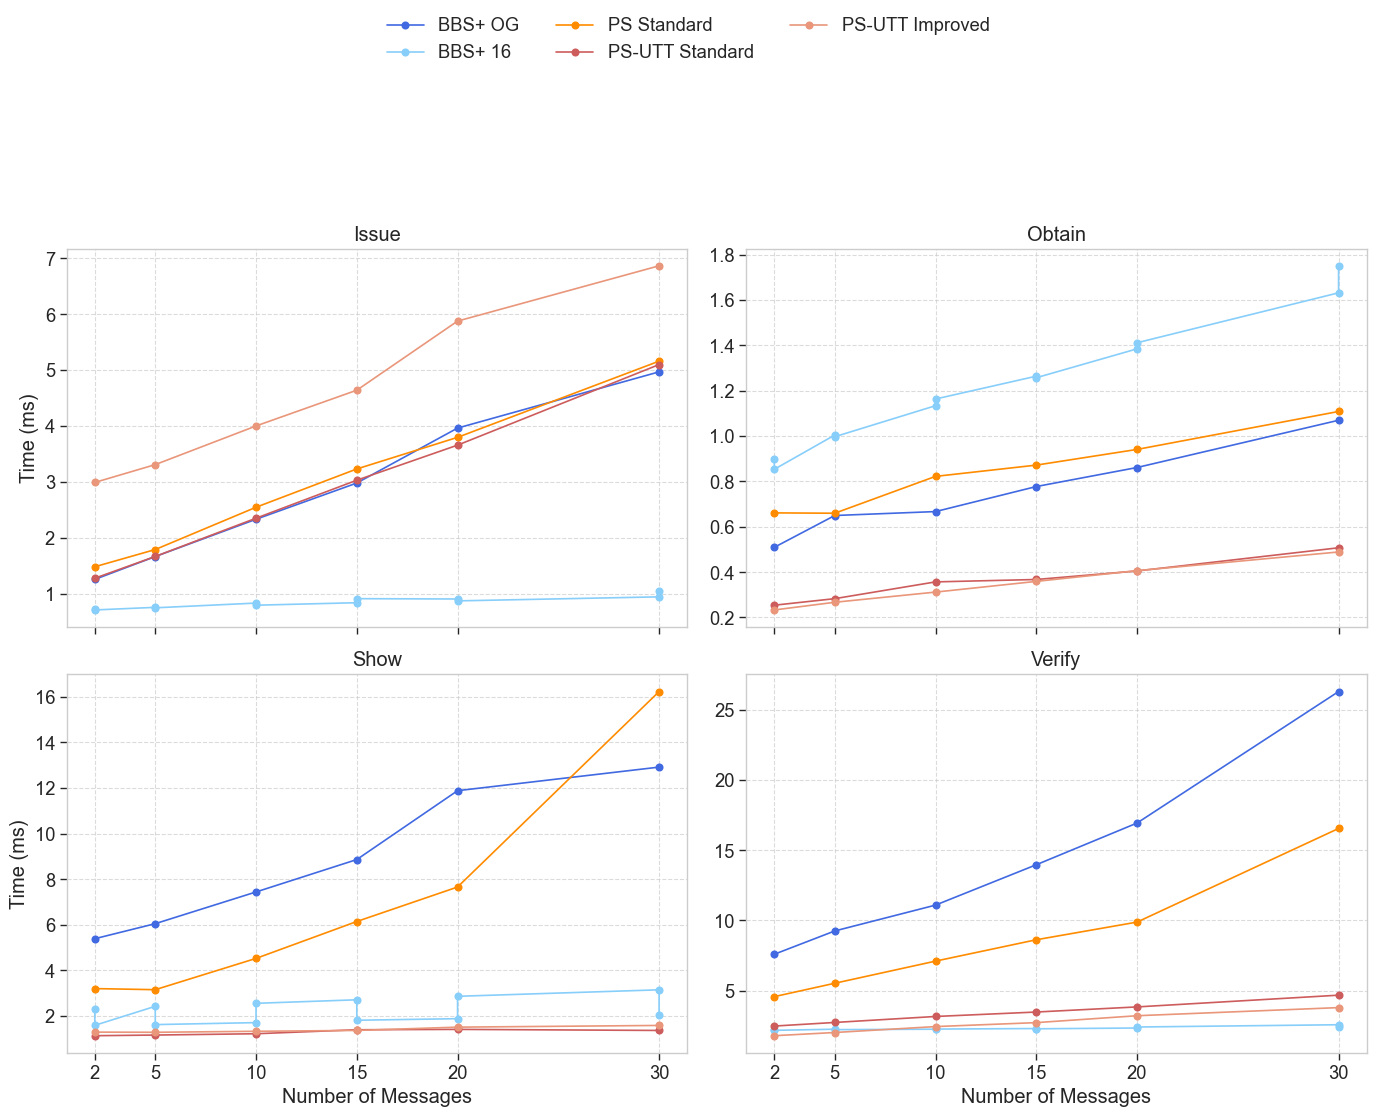
\includegraphics[width=1\linewidth]{comparison-line-graph.png}
    \caption{Performance Comparison of Anonymous Credential Schemes}
    
\end{figure}

\begin{figure}
    \centering
    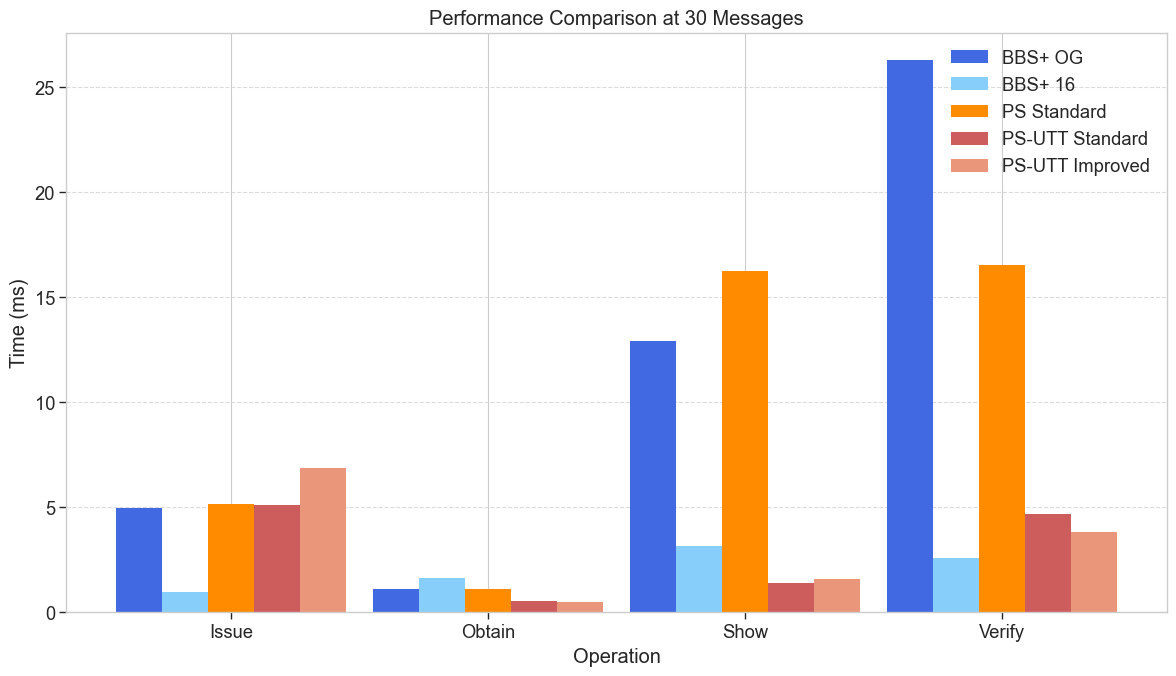
\includegraphics[width=0.7\linewidth]{performance-30.png}
    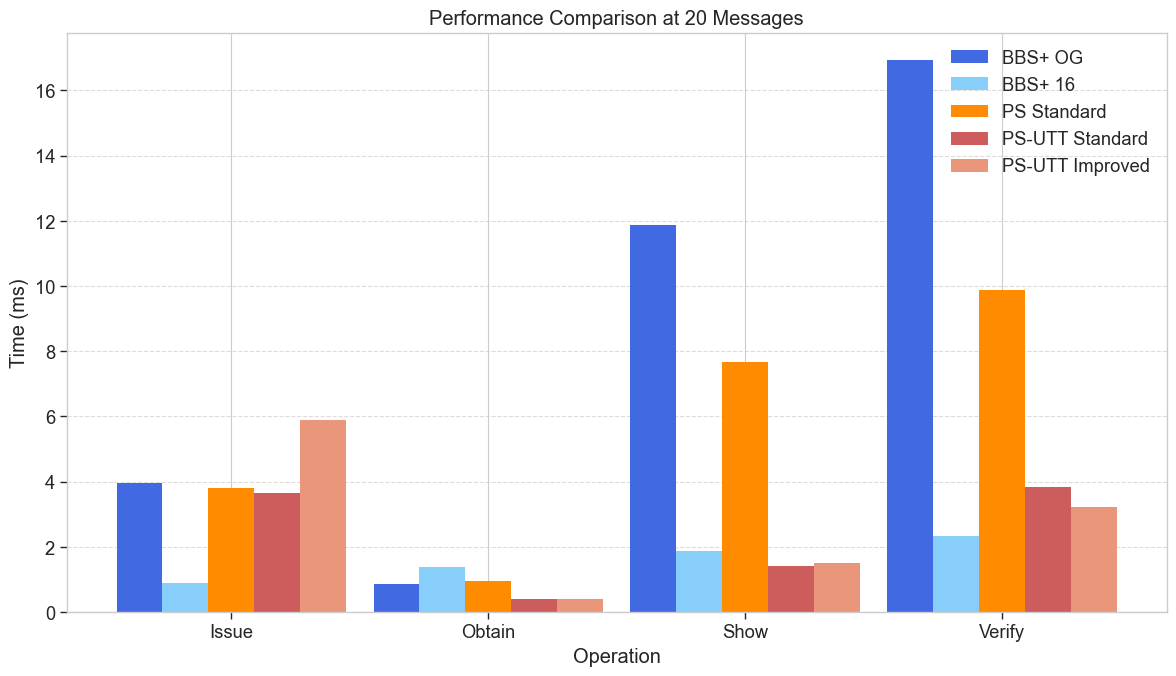
\includegraphics[width=0.7\linewidth]{performance-20.png}
    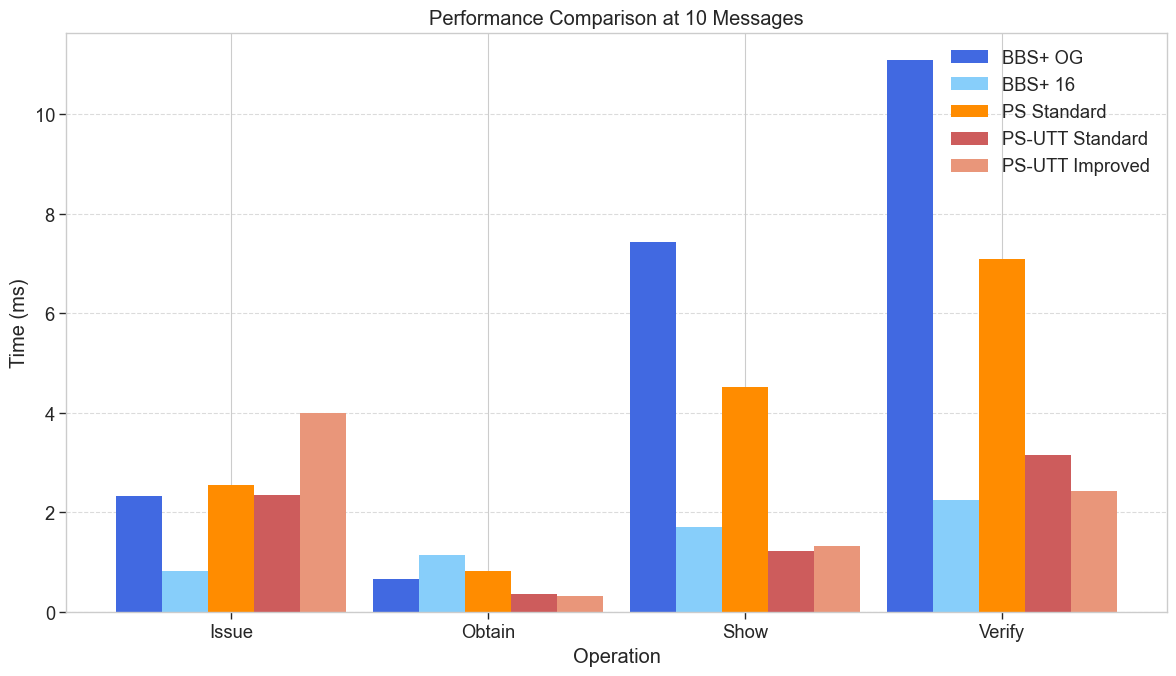
\includegraphics[width=0.7\linewidth]{performance-10.png}
     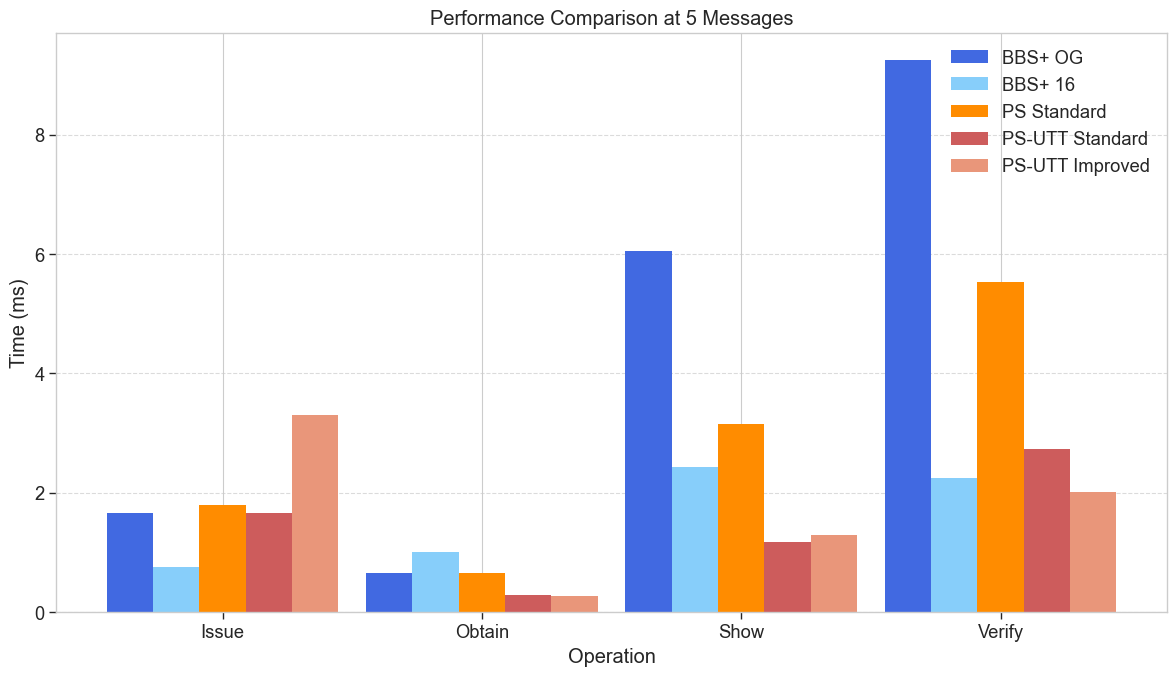
\includegraphics[width=0.7\linewidth]{performance-5.png}
    \caption{Performance Comparison of Anonymous Credential Schemes}
    
\end{figure}




% \subsubsection{Case Study: Credential Expiration Verification}

% To demonstrate the practical impact of our optimizations, we compared our approach against alternative systems for the common use case of verifying credential expiration. Table~\ref{tab:expiry-comparison} presents the results for generating and verifying a proof that a credential has not expired.

% \begin{table}[htbp]
% \centering
% \caption{Performance Comparison for Credential Expiration Verification}
% \label{tab:expiry-comparison}
% \begin{tabular}{lrrr}
% \toprule
% \textbf{Approach} & \textbf{Show (ms)} & \textbf{Verify (ms)} & \textbf{Proof Size} \\
% \midrule
% Simple Possession & 2 & 2 & 424B \\
% Expiry (ZK-Creds) & 50 & \multirow{3}{*}{$\left\}5\text{ ms}\right.$} & \multirow{3}{*}{744B} \\
% Linkable Show (ZK-Creds) & 41 &  &  \\
% Rate Limiting (ZK-Creds) & 58 &  &  \\
% \textbf{Our Approach} & \textbf{1.3} & \textbf{2.0} & \textbf{512B} \\
% \bottomrule
% \end{tabular}
% \end{table}

% Our evaluation reveals that our system can verify a credential's expiry status in just 3.3ms (combined Show+Verify), compared to 45-55ms for ZK-Creds approaches—a performance improvement of over 13×. This dramatic difference highlights how our optimized signature scheme and sigma protocol enables efficient predicate verification without sacrificing privacy.

% Importantly, while general-purpose zero-knowledge systems provide flexibility, they introduce substantial computational overhead that makes interactive verification scenarios impractical. Our approach achieves similar expressiveness with dramatically better performance for the most common credential verification operations.

















  \chapter{Identity Binding Multi Issuer Multi Credential Anonymous Credentials}\label{chap3}

\section{Introduction}\label{sec:mimc}
Anonymous credential systems enable users to prove statements about their attributes while preserving privacy, evolving from single-issuer designs (e.g., Idemix~\cite{camenisch_design_2002}) to meet complex, real-world demands. Unlike Chapter 2's single-issuer $\ABC$ system, we address the problem \emph{how can users privately combine credentials from multiple, mutually distrusting issuers to prove they belong to the same identity, without revealing it?}

Consider a user proving they hold (1) a government-issued ID confirming residency, (2) an employer credential verifying income, and (3) a training certificate—all tied to one identity, without linking them via a public identifier. Alternatively, in content credentialing, a user might present images signed by different devices (e.g., cameras) to a journal, proving they share an account while selectively disclosing metadata. Existing approaches fall short: attribute-based signatures lack aggregation~\cite{cimato_signature_2003}, aggregate signatures assume a single issuer \cite{goos_short_2001, hutchison_short_2004} or limit revocation flexibility~\cite{galdi_traceable_2022}, and generic zkSNARKs, while expressive, incur high computational costs~\cite{rosenberg_zk-creds_2022}. CanDID~\cite{maram_candid_2020} binds credentials via a consistent name, but this offers weaker security against malicious issuers and their system lacks issuer-privacy for internal identifiers. ZKcreds~\cite{rosenberg_zk-creds_2022} uses a zkSNARK-based join gadget for multi-credential proofs, yet its proof computation scales poorly, especially for multiple credentials. Our Multi-Issuer Multi-Credential Anonymous Credential system (MIMC-ABC) overcomes these limitations with a secure, efficient solution.

MIMC-ABC employs position-binding commitments and zero-knowledge proofs to cryptographically bind credentials from distinct issuers to a single, private identifier, ensuring anonymity and unforgeability even against colluding adversaries. We formalize a security model for multi-issuer identity binding, define the identity binding property, and provide rigorous proofs of its guarantees. Our comprehensive attack taxonomy—covering forgery, predicate manipulation, and binding attacks—demonstrates robustness, while a scaling analysis shows security holds as issuers and credentials grow. Performance evaluations reveal that privacy-preserving multi-issuer verification, though roughly 3× slower than non-private baselines (e.g., 18.67ms vs. 6.77ms for 4 credentials), remains efficient for practical use.

\subsection{Contributions}
This chapter advances the state of anonymous credentials with:
\begin{itemize}
    \item A formalized multi-issuer security model with an identity binding property, ensuring credentials from distinct issuers provably belong to the same user without compromising anonymity
    \item Security proofs showing resilience as the number of issuers and credentials increases.
    \item A performance evaluation methodology comparing non-private, private single-issuer (with batch verification), and private multi-issuer scenarios, quantifying privacy’s overhead.
\end{itemize}


\begin{figure}
    \centering
    \scalebox{0.85}{ % Scale down the entire figure
        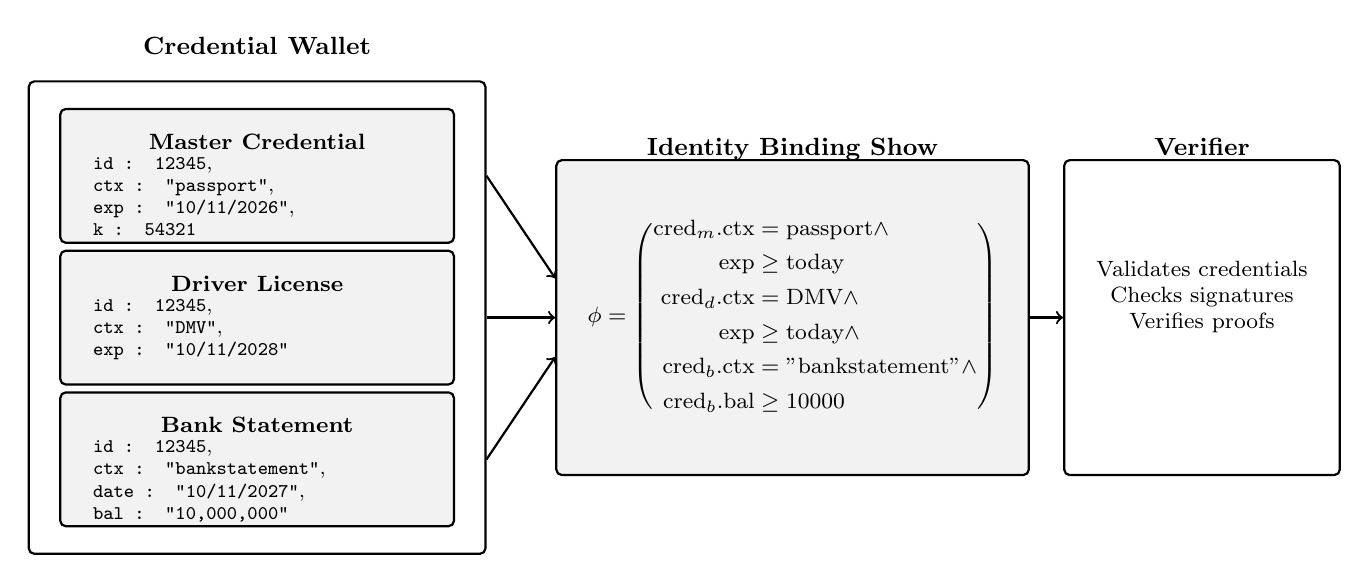
\begin{tikzpicture}[
            box/.style={draw, rounded corners=2pt, minimum width=5.8cm, minimum height=6cm}, % Increased height
            smallbox/.style={draw, rounded corners=2pt, fill=gray!10, minimum width=5cm, minimum height=1.7cm}, % Slightly larger
            verifierbox/.style={draw, rounded corners=2pt, minimum width=3.5cm, minimum height=4cm},
            showbox/.style={draw, rounded corners=2pt, fill=gray!10, minimum width=6cm, minimum height=4cm},
            thick
        ]
        
        % Digital Credential Wallet
        \node[box] (wallet) at (0,0) {};
        \node[anchor=south, font=\bfseries\small] at ($(wallet.north) + (0,0.2)$) {Credential Wallet};
        
        % Master Credential
        \node[smallbox] (master) at (0,1.8) {}; % Adjusted position for 1cm spacing
        \node[anchor=north, font=\footnotesize\bfseries] at ($(master.north) + (0,-0.2)$) {Master Credential};
        
        \node[anchor=north west, font=\scriptsize, align=left] at ($(master.north west) + (0.3,-0.5)$) {
            \texttt{id : 12345}, \\
            \texttt{ctx : "passport"}, \\
            \texttt{exp : "10/11/2026"}, \\
            \texttt{k : 54321}
        };
        
        % Driver License Credential
        \node[smallbox] (driver) at (0,0) {}; % Center position
        \node[anchor=north, font=\footnotesize\bfseries] at ($(driver.north) + (0,-0.2)$) {Driver License};
        
        \node[anchor=north west, font=\scriptsize, align=left] at ($(driver.north west) + (0.3,-0.5)$) {
            \texttt{id : 12345}, \\
            \texttt{ctx : "DMV"}, \\
            \texttt{exp : "10/11/2028"}
        };
        
        % Bank Statement Credential
        \node[smallbox] (bank) at (0,-1.8) {}; % Adjusted position for 1cm spacing
        \node[anchor=north, font=\footnotesize\bfseries] at ($(bank.north) + (0,-0.2)$) {Bank Statement};
        
        \node[anchor=north west, font=\scriptsize, align=left] at ($(bank.north west) + (0.3,-0.5)$) {
            \texttt{id : 12345}, \\
            \texttt{ctx : "bankstatement"}, \\
            \texttt{date : "10/11/2027"}, \\
            \texttt{bal : "10,000,000"}
        };
        
        % Identity Binding Show
        \node[showbox] (show) at (6.8,0) {}; % Slightly adjusted x-position
        \node[anchor=north, font=\small\bfseries] at ($(show.north) + (0,0.4)$) {Identity Binding Show};
        
        \node[font=\footnotesize] at ($(show.north) + (0,-2)$) 
        {$\phi = \left(\begin{aligned}
         \textrm{cred}_m.\textrm{ctx} &= \textrm{passport} \wedge\\
          \textrm{exp} &\geq \textrm{today} \\
         \textrm{cred}_d.\textrm{ctx} &= \textrm{DMV} \wedge \\
         \textrm{exp} &\geq \textrm{today} \wedge\\
         \textrm{cred}_b.\textrm{ctx} &= \textrm{"bankstatement"} \wedge\\
         \textrm{cred}_b.\textrm{bal} &\geq 10000
        \end{aligned}\right)$};
        
        % Verifier box 
        \node[verifierbox] (verifier) at (12,0) {}; % Adjusted x-position
        \node[anchor=north, font=\small\bfseries] at ($(verifier.north) + (0,0.4)$) {Verifier};
        
        % Draw contents for the verifier box
        \node[font=\footnotesize, align=center] at ($(verifier.north) + (0,-1.75)$) {
            Validates credentials\\
            Checks signatures\\
            Verifies proofs
        };
        
        % Arrows from wallet edge to credential show
        \draw[->, thick] ($(wallet.east) + (0,1.8)$) -- ($(show.west) + (0,0.5)$);
        \draw[->, thick] ($(wallet.east) + (0,0)$) -- (show.west);
        \draw[->, thick] ($(wallet.east) + (0,-1.8)$) -- ($(show.west) + (0,-0.5)$);
        
        % Arrow from credential show to verifier
        \draw[->, thick] (show.east) -- (verifier.west);
        
        \end{tikzpicture}
    }
    \caption[Credential Showing Scheme]{A credential showing scheme for privacy-preserving protocols, illustrated with a credential hierarchy binding multiple credentials (passport, driver's license, bank statement) to enable secure and privacy-preserving presentation to verifiers.}
    \label{fig:credential-show-revised}
\end{figure}




\section{System Model and Definitions}

Our Multi-Issuer Multi-Credential Anonymous Credential (MIMC-ABC) system extends the single-issuer Attribute-Based Anonymous Credential (ABC) framework from Chapter 2 to support credentials from multiple, mutually distrusting issuers, bound to a single identity. The ABC system uses a variant of rerandomizable Pointcheval-Sanders signatures~\cite{sako_short_2016} and position-binding Pedersen commitments~\cite{tomescu_utt_2022} to enable expressive predicate proofs over attributes. MIMC-ABC builds on this by introducing multi-issuer key generation and a cryptographic identity binding mechanism, ensuring all credentials verifiably belong to the same user without revealing their identity.

\subsection{MIMC-ABC Syntax}

A MIMC-ABC system consists of the following probabilistic polynomial-time (PPT) algorithms, parameterized by a security parameter $\lambda$ and attribute vector length $\ell$:

\begin{definition}[MIMC-ABC]
    \begin{itemize}
    \item $\mathsf{Setup}(1^\lambda) \to \mathsf{pp}$: Outputs public parameters $\mathsf{pp}$, including a bilinear group $\BG = (\G_1, \G_2, \G_T, e, g, \tilde{g}, p)$ as in Section 2.1.
    
    \item $\mathsf{OrgKeyGen}(\mathsf{pp}, \ell, j) \to (\mathsf{osk}_j, \mathsf{opk}_j)$: For issuer $j$, takes $\mathsf{pp}$ and $\ell$, outputs a keypair $(\mathsf{osk}_j, \mathsf{opk}_j)$ using the signature scheme from Section 2.3.

    \item $(\mathsf{Obtain}(\attrs, \{\mathsf{opk}_j\}_j, \mathsf{aux}), \mathsf{Issue}(\mathsf{osk}_j, \mathsf{cm}, \mathsf{aux})) \to (\mathsf{cred}_j, \bot)$: An interactive protocol between a user and issuer $j$. The user inputs an attribute vector $\attrs = [\id, \ctx_j, \exp_j]$, where $\id$ is a unique identifier, $\ctx_j$ is the issuer-specific context, and $\attrs_j$ are attributes. The user samples $\usk_j \sample \Z_p$, commits as $\mathsf{cm} \gets \mathsf{CM.Com}(\attrs; \usk_j)$, and proves its opening (Section 2.4.3). The issuer signs $\mathsf{cm}$ with $\mathsf{osk}_j$, outputting $\mathsf{cred}_j = (\sigma_j, \mathsf{cm})$ to the user and $\bot$ to itself.

    \item $(\mathsf{Show}(\{\mathsf{cred}_j\}_j, \{\usk_j\}_j, \phi), \mathsf{Verify}(\{\mathsf{cred}_j'\}_j, \pi)) \to \{0,1\}$: An interactive protocol between a user and verifier. The user inputs a set of credentials $\{\mathsf{cred}_j\}_j$ from (optionally) distinct issuers, rerandomizes each $(\sigma_j, \mathsf{cm})$ to $(\sigma_j', \mathsf{cm}')$, and computes a proof $\pi$ that $\phi(\{\attrs_j\}_j) = 1$ and all $\id$ values match, using $\Sigma$-protocols. The verifier checks the proof and rerandomized credentials against $\{\mathsf{opk}_j\}_j$, outputting 1 if valid, 0 otherwise.
\end{itemize}
\end{definition}


\subsection{Security Properties}

MIMC-ABC inherits the core security properties from the ABC system—correctness, unforgeability, and anonymity (Section 2.5)—and adds identity binding for the multi-issuer setting:

\begin{itemize}
    \item \textbf{Correctness}: An honest user with valid credentials from multiple issuers can generate a proof for any predicate $\phi$ their attributes satisfy, including same-identity constraints, which verifies with probability $1 - \negl(\lambda)$.
    
    \item \textbf{Unforgeability}: No PPT adversary can produce a valid proof for a predicate $\phi$ they cannot legitimately satisfy, including forging credentials or mixing credentials from different identities, except with negligible probability.
    
    \item \textbf{Anonymity}: Proofs reveal only that $\phi$ is satisfied, not the user’s identity or credential details, even if all issuers and the verifier collude.
    
    \item \textbf{Identity Binding}: When $\phi$ requires all credentials to share the same $\id$, no PPT adversary can produce a valid proof using credentials with differing $\id$ values, except with negligible probability.
\end{itemize}

\subsection{Identity Binding Property}

We formalize identity binding as a distinct security property for multi-issuer systems:



\begin{definition}[Identity Binding]
A MIMC-ABC system satisfies identity binding if for all PPT adversaries $\mathcal{A}$, there exists a negligible function $\mathsf{negl}$ such that:
\[
\Pr\left[
\begin{array}{l}
    \mathsf{pp} \gets \mathsf{Setup}(1^\lambda) \\
    \{(\mathsf{osk}_j, \mathsf{opk}_j)\}_j \gets \mathsf{OrgKeyGen}(\mathsf{pp}, \ell) \\
    (\{\mathsf{cred}_j'\}_j, \phi^*, \pi^*) \gets \mathcal{A}^{\mathcal{O}}(\{\mathsf{opk}_j\}_j)
\end{array}
: \begin{array}{l}
    \mathsf{Verify}(\{\mathsf{cred}_j'\}_j, \phi^*, \pi^*) = 1 \land \\
    \phi^* \text{ requires } \forall j, \id_j = \id \land \\
    \exists j, k: \id_j \neq \id_k
\end{array}
\right] \leq \mathsf{negl}(\lambda)
\]
where $\mathcal{O}$ includes oracles for honest user creation, corruption, credential issuance, and proof generation (adapted from Section 2.5).
\end{definition}

This ensures that credentials presented together must share a single, private $\id$, enforced via position-binding commitments and zero-knowledge proofs, as detailed in Section 3.













\section{Construction}

Our MIMC-ABC system constructs credentials as rerandomizable Pointcheval-Sanders signatures from \cite{tomescu_utt_2022} over position-binding Pedersen commitments, extending the single-issuer ABC system (Section 2.4) to bind credentials from multiple issuers to a shared, private identifier. We leverage the algebraic structure of these primitives and $\Sigma$-protocols to prove credential validity and identity consistency efficiently, supporting predicates over an arbitrary number of attributes.

\subsection{Intuition}

Each credential from issuer $j$ commits to an attribute vector $\attrs_j = [\id, \ctx_j, \exp_j]$, where $\id$ is a unique, user-chosen identifier, $\ctx_j$ denotes the credential’s context (e.g., "passport"), and $\exp_j$ is an expiration date. The vector can extend to additional attributes as needed (e.g., income, degree, date of birth). 

Each credential from issuer $j$ commits to an attribute vector $\attrs_j = [\id, \ctx_j, \exp_j]$, where $\id$ is a unique, user-chosen identifier, $\ctx_j$ denotes the credential’s context (e.g., "passport"), and $\exp_j$ is an expiration date. The vector can extend to additional attributes as needed (e.g., income, degree). Issuance is flexible: the user privately commits to $\mathsf{cm}_1 = \mathsf{CM.Com}([\id, 0, 0]; \usk_j)$ with randomness $\usk_j$ and proves its opening and proves it commits to zero's in positions 2, 3, while issuer $j$ commits to $\mathsf{cm}_2 = \mathsf{CM.Com}([0, \ctx_j, \exp_j]; 0)$ and homomorphically combines them into $\mathsf{cm}_j = \mathsf{cm}_1 \cdot \mathsf{cm}_2 = \mathsf{CM.Com}([\id, \ctx_j, \exp_j]; \usk_j)$, signing it. Alternatively, the user can commit to all attributes privately, and the issuer signs directly, supporting both fully private and issuer-driven scenarios (e.g., credential oracles like DECO~\cite{zhang_deco_2020}). To present credentials, the user rerandomizes each signature and commitment, then proves in zero-knowledge that: (1) all signatures are valid under their respective issuer keys, and (2) all commitments share the same $\id$, satisfying a predicate $\phi$.

For example, consider a user with credentials from three issuers ($j = 1, 2, 3$): a passport, driver’s license, and university degree, each with the same $\id = 12345$ (Figure~\ref{fig:three-creds}). The user rerandomizes each pair $(\sigma_j, \mathsf{cm}_j)$ to $(\sigma_j', \mathsf{cm}_j')$ and proves they meet a policy, e.g., $\phi = (\ctx_1 = \text{"passport"} \land \exp_1 > \text{today} \land \ctx_2 = \text{"dmv"} \land \ctx_3 \in \mathcal{D})$, where $\mathcal{D}$ is a set of accredited universities.

\begin{figure}[h]
    \centering
    \begin{pchstack}[boxed, center, space=4em]
        \begin{pcvstack}
            \procedure[space=auto]{Passport ($j=1$)}{
                \id: 12345, \\
                \ctx_1: "passport", \\
                \exp_1: "10/11/2026"
            }
        \end{pcvstack}
        \pcvspace
        \begin{pcvstack}
            \procedure[space=auto]{Driver’s License ($j=2$)}{
                \id: 12345, \\
                \ctx_2: "dmv", \\
                \exp_2: "05/01/2027"
            }
        \end{pcvstack}
        \pcvspace
        \begin{pcvstack}
            \procedure[space=auto]{University Degree ($j=3$)}{
                \id: 12345, \\
                \ctx_3: "usyd-bcompsc", \\
                \exp_3: "12/31/2024"
            }
        \end{pcvstack}
    \end{pchstack}
    \caption{Example credentials from three issuers, sharing $\id = 12345$. Additional attributes (e.g., degree type) can be included.}
    \label{fig:three-creds}
\end{figure}

\subsection{Construction Details}

The MIMC-ABC system operates as follows, reusing primitives from Chapter 2 (Sections 2.3, 2.4):

\begin{itemize}
    \item $\mathsf{Setup}(1^\lambda)$: Generates $\mathsf{pp}$ with bilinear group $\BG = (\G_1, \G_2, \G_T, e, g, \tilde{g}, p)$ and commitment generators $(g_1, g_2, g_3, \tilde{g}_1, \tilde{g}_2, \tilde{g}_3)$ for $\ell = 3$, extensible to more attributes.
    
    \item $\mathsf{OrgKeyGen}(\mathsf{pp}, \ell, j)$: Issuer $j$ runs $\mathsf{RS.KeyGen}$ (Section 2.3) to produce $(\mathsf{osk}_j, \mathsf{opk}_j)$, with $\mathsf{opk}_j = (\vk_j, \ck_j)$.

    \item $\mathsf{Obtain}$ and $\mathsf{Issue}$: The user commits $\mathsf{cm}_j = \mathsf{CM.Com}([\id, \ctx_j, \exp_j]; \usk_j)$, proves its opening via $\pircom$ (Section 2.4.3), and sends it to issuer $j$. Issuer $j$ signs it as $\sigma_j = \mathsf{RS.Sign}(\mathsf{cm}_j, \mathsf{osk}_j)$, returning $\mathsf{cred}_j = (\sigma_j, \mathsf{cm}_j)$. The user retains $\usk_j$.

    \item $\mathsf{Show}$ and $\mathsf{Verify}$: For credentials $\{\mathsf{cred}_j\}_j$, the user:
        \begin{enumerate}
            \item Rerandomizes: $\mathsf{cm}_j' = \mathsf{CM.Rerand}(\mathsf{cm}_j, \Delta_{r_j})$, $\sigma_j' = \mathsf{RS.Rerand}(\sigma_j, \Delta_{r_j}, \Delta_{u_j})$.
            \item Proves via $\Sigma$-protocol:
                \[
                \mathcal{R}_\phi =\left\{ 
                \begin{array}{l} 
                (\{\mathsf{cm}_j', \sigma_j'\}_j, (\id, \{\ctx_j, \exp_j, \usk_j + \Delta_{r_j}\}_j)) \\
                \end{array} 
                \middle|
                \begin{array}{l}
                \forall j: \mathsf{RS.Ver}(\sigma_j', \mathsf{cm}_j', \vk_j) = 1 \land \\
                \mathsf{cm}_j' = g_1^\id g_2^{\ctx_j} g_3^{\exp_j} g^{\usk_j + \Delta_{r_j}} \land \\
                \phi(\{\ctx_j, \exp_j\}_j) = 1
                \end{array} 
                \right\}
                \]
        \end{enumerate}
        The verifier checks $\pi$ and $\{\mathsf{opk}_j\}_j$, accepting if valid.
\end{itemize}



\subsection{Identity Binding Mechanism}

Identity binding relies on the position-binding property of Pedersen commitments (Section 2.2). The $\Sigma$-protocol proves that all $\mathsf{cm}_j'$ share the same $\id$ in the first position ($g_1^\id$), using an equality proof across commitments:
\[
\rid = \zkpok \left\{ 
\begin{array}{l} 
(\{\mathsf{cm}_j'\}_j, (\id, \{\usk_j', \ctx_j, \exp_j\}_j)) \\
\end{array} 
\middle|
\begin{array}{l}
\forall j: \mathsf{cm}_j' = g_1^\id g_2^{\ctx_j} g_3^{\exp_j} g^{\usk_j'}
\end{array} 
\right\}
\]
The position-binding assumption (SDLP, Section 2.1) ensures an adversary cannot forge commitments with different $\id$ values that appear equal, reducing security to standard cryptographic hardness.






\section{Security Analysis}

We analyze the security of MIMC-ABC against a PPT adversary controlling issuers, corrupting users, and querying oracles (adapted from Section 2.5). Our system inherits the ABC framework’s guarantees (Section 2.6) and strengthens them with identity binding for the multi-issuer setting. We prove correctness informally, then formalize unforgeability, anonymity, and identity binding, reducing security to the underlying primitives’ assumptions: EUF-CMA of the signature scheme (Section 2.3), position-binding of the commitment scheme (Section 2.2), and soundness of $\Sigma$-protocols (Section 2.4.3).

\subsection{Correctness}

An honest user with valid credentials $\{\mathsf{cred}_j\}_j$ from issuers $\{j\}$ can always generate a proof $\pi$ for a predicate $\phi$ their attributes $\{\attrs_j\}_j = \{[\id, \ctx_j, \exp_j]\}_j$ satisfy, including same-$\id$ constraints. Rerandomization ensures signatures and commitments verify under $\{\mathsf{opk}_j\}_j$, and the $\Sigma$-protocol proves $\phi$ and $\id$ equality with probability $1 - \negl(\lambda)$, following Section 2.6’s correctness argument extended to multiple issuers.

\subsection{Unforgeability}

\begin{theorem}[Unforgeability]
MIMC-ABC is unforgeable if the rerandomizable signature scheme is EUF-CMA secure, the Pedersen commitment scheme is position-binding, and the $\Sigma$-protocol is sound. For any PPT adversary $\mathcal{A}$, $\Adv^{\mathsf{UNF}}_{\MIMCABC, \mathcal{A}}(\lambda) \leq \negl(\lambda)$.
\end{theorem}

\begin{proof}[Sketch]
We reduce unforgeability to three cases, adapting Section 2.6’s ABC proof:
\begin{enumerate}
    \item \textbf{Forged Signature}: If $\mathcal{A}$ outputs a valid $\mathsf{cred}_j' = (\sigma_j', \mathsf{cm}_j')$ not issued by any $\mathsf{osk}_j$, we extract $\sigma_j'$ as an EUF-CMA forgery.
    \item \textbf{Predicate Misuse}: If $\mathcal{A}$ uses valid credentials but proves a false $\phi^*$ (e.g., $\exp_j < \text{today}$ when $\exp_j > \text{today}$), the $\Sigma$-protocol’s special soundness lets us extract a witness contradicting the original attributes, breaking position-binding.
    \item \textbf{Identity Mixing}: If $\mathcal{A}$ combines credentials with different $\id$ values yet proves same-$\id$, we extract two openings of some $\mathsf{cm}_j'$ (e.g., $g_1^{\id_1}$ vs. $g_1^{\id_2}$), breaking position-binding.
\end{enumerate}
A reduction $\mathcal{B}$ simulates the game (Section 2.5), embedding EUF-CMA and position-binding challenges into $\{\mathsf{opk}_j\}_j$ and $\mathsf{cm}_j$. Any forgery violates one assumption, bounding $\mathcal{A}$’s advantage by $\negl(\lambda)$.
\end{proof}

\subsection{Anonymity}

\begin{theorem}[Anonymity]
MIMC-ABC is anonymous, even against colluding issuers, if the signature scheme’s rerandomization is indistinguishable, the commitment scheme is hiding, and the $\Sigma$-protocol is zero-knowledge. For any PPT adversary $\mathcal{A}$, $\Adv^{\mathsf{ANON}}_{\MIMCABC, \mathcal{A}}(\lambda) \leq \negl(\lambda)$.
\end{theorem}

\begin{proof}[Sketch]
We use a hybrid argument, extending Section 2.6’s ABC anonymity proof:
\begin{itemize}
    \item \textbf{Hybrid 0}: Real game with user $i_b$’s credentials $\{\mathsf{cred}_j\}_j$, rerandomized and proven via $\mathsf{Show}$.
    \item \textbf{Hybrid 1}: Replace $\pi$ with a simulated proof using the $\Sigma$-protocol’s zero-knowledge simulator.
\end{itemize}
The hiding property of Pedersen commitments ensures $\mathsf{cm}_j'$ is uniform, signature rerandomization makes $\sigma_j'$ indistinguishable from fresh signatures, and the simulated $\pi$ hides $i_b$, even if all issuers share $\{\mathsf{osk}_j\}_j$. The advantage is negligible as hybrids are computationally indistinguishable.
\end{proof}

\subsection{Identity Binding}

\begin{theorem}[Identity Binding]
MIMC-ABC satisfies identity binding under the SDLP assumption (Section 2.1). For any PPT adversary $\mathcal{A}$ mixing credentials with distinct $\id$ values, $\Adv^{\mathsf{BIND}}_{\MIMCABC, \mathcal{A}}(\lambda) \leq n \cdot m \cdot \Adv^{\mathsf{SDLP}}(\lambda) + \negl(\lambda)$, where $n$ is the number of issuers and $m$ is credentials per user.
\end{theorem}

\begin{proof}[Sketch]
If $\mathcal{A}$ outputs $\{\mathsf{cred}_j'\}_j$, $\phi^*$ requiring same $\id$, and $\pi^*$ verifying despite $\id_j \neq \id_k$ for some $j, k$, the $\Sigma$-protocol’s special soundness extracts witnesses from $\pi^*$. For each $\mathsf{cm}_j' = g_1^{\id_j} g_2^{\ctx_j} g_3^{\exp_j} g^{\usk_j'}$, we get $\id_j$, and differing $\id$ values imply two openings of some $\mathsf{cm}_j'$ at position 1 (e.g., $g_1^{\id_1}$ vs. $g_1^{\id_2}$). A reduction $\mathcal{B}$ embeds an SDLP challenge $(g^x, \tilde{g}^x)$ into $g_1, \tilde{g}_1$, solving $x$ with probability $1/(n \cdot m)$ per credential, yielding the bound.
\end{proof}

\subsection{Security Scaling}

The identity binding advantage scales linearly with $n$ and $m$, reflecting the number of opportunities to break position-binding. This graceful degradation ensures MIMC-ABC remains secure as the system grows, a key advantage over prior multi-issuer schemes lacking formal binding guarantees.

\section{Identity Binding Application: Efficient KYC/AML Identity Verification}

\todonote{Sam to do}
Speak about the KYC/AML process and why identity binding is necessary


\section{Performance Evaluation}

We evaluate MIMC-ABC to quantify the overhead of privacy-preserving multi-issuer credential verification, comparing it against non-private and single-issuer baselines. Unlike prior multi-issuer systems (e.g., CanDID~\cite{maram_candid_2020}, ZKcreds~\cite{rosenberg_zk-creds_2022}), MIMC-ABC balances strong identity binding with practical efficiency, leveraging our signature optimization \ref{subsec:g2_verify_speedup}. Our benchmarks focus on verification time—the critical path in authentication—across three scenarios: non-private, private single-issuer with batch signature aggregation, and private multi-issuer.

\subsection{Methodology}

We implemented MIMC-ABC using the arkworks library~\cite{arkworks_contributors_arkworks_2022} on a BLS12-381 curve (128-bit security), running on a MacBook Air M2 (16GB RAM, macOS Sequoia 15.3.2). We measure verification time for 4, 16, and 32 credentials, each with 4 attributes, averaging 100 trials (standard deviation < 5\%). Scenarios include:
\begin{enumerate}
    \item \textbf{Non-Private}: Signatures verified with batch aggregation, revealing $\attrs_j$ in the clear—a common baseline for non-anonymous systems.
    \item \textbf{Private Single-Issuer}: All credentials from one issuer, using batch verification of PS signatures (Section 2.3) and a $\Sigma$-protocol for same-$\id$ and predicate satisfaction.
    \item \textbf{Private Multi-Issuer}: Each credential from a different issuer, requiring individual signature verification and a $\Sigma$-protocol for identity binding (worst-case scenario).
\end{enumerate}




\begin{figure}
    \centering
   
    % Bottom row with 2x2 grid of smaller figures
    \begin{minipage}{0.48\textwidth}
        \centering
        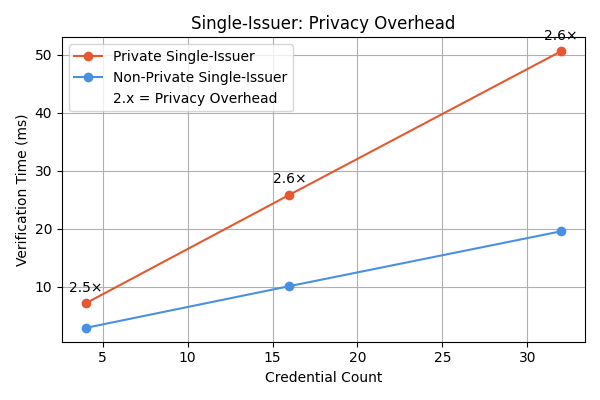
\includegraphics[width=\textwidth]{figures/chap3_single_issuer_privacy_overhead.png}
    \end{minipage}
    \hfill
    \begin{minipage}{0.48\textwidth}
        \centering
        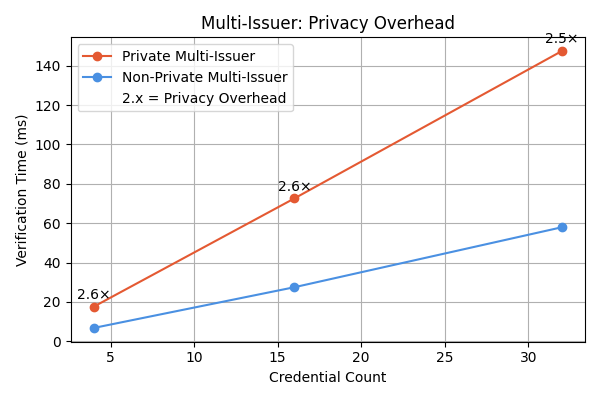
\includegraphics[width=\textwidth]{figures/chap3_multi_issuer_privacy_overhead.png}
    \end{minipage}
    
    \caption[The Cost of Privacy for Multi-Credential Verifiable Presentations]{These graphs show the cost of privacy for single-issuer (left) and multi-issuer(right) credential use with multiple credentials. The graph shows a 2.6x increase in Show+Verify time for private multi-credential use. The left graph shows single-issuer multi-credential verification (with batch verification). The right graph shows multi-issuer multi-credential verification (no batch verification). Both graphs use a credential with 16 attributes displaying Show+Verify time.}
    \label{fig:chap3_privacy_overhead_graphs}
\end{figure}




\begin{figure}
    \centering
   
    % Bottom row with 2x2 grid of smaller figures
    \begin{minipage}{0.48\textwidth}
        \centering
        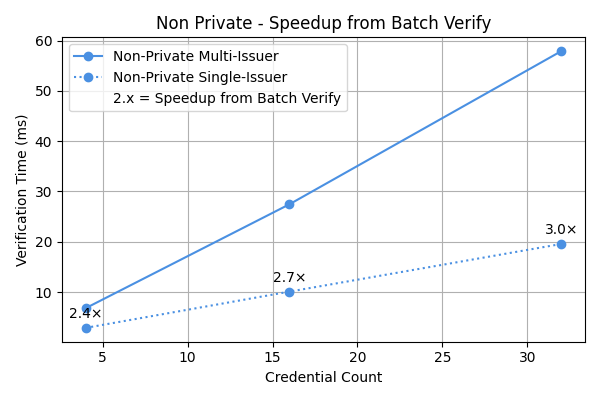
\includegraphics[width=\textwidth]{figures/chap3_nonprivate_batch_speedup.png}
    \end{minipage}
    \hfill
    \begin{minipage}{0.48\textwidth}
        \centering
        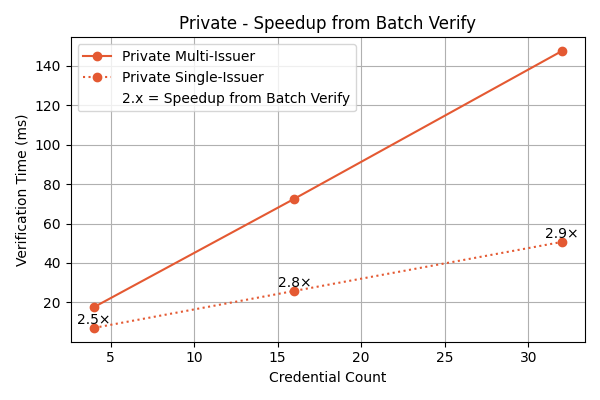
\includegraphics[width=\textwidth]{figures/chap3_private_batch_speedup.png}
    \end{minipage}
    
    \caption[Signature Aggregation/Batch Verification Speedup for Multi-Credential Verifiable Presentations]{These graphs show the benefit of single-issuer signature aggregation, but also show that multi-issuer credential verification adds small 2.4x-3x overhead and therefore does not impact the Show+Verify significantly}
    \label{fig:chap3_batch_verify_improvements}
\end{figure}




\begin{table}[ht]
\centering
\caption{Varying Credential Count, Set Attribute Number (4) (time in ms)}
\label{tab:performance-credentialscaling-chap3}
\begin{tabular}{l@{\hspace{1em}}r@{\hspace{0.5em}}r@{\hspace{0.5em}}r@{\hspace{0.5em}}r@{\hspace{1em}}r}
\toprule
\textbf{Scenario} & \multicolumn{3}{c}{\textbf{Verify (ms)}} & \textbf{Overhead Avg.} & \textbf{Notes} \\
\cmidrule(lr){2-4}
& \textbf{4 Creds} & \textbf{16 Creds} & \textbf{32 Creds} &  & \\
\midrule
Non-Private Single-Issuer & 2.87 & 10.08 & 19.55 & -- & Cleartext, batched \\
Private Single-Issuer & 7.11 & 25.85 & 50.64 & 2.5× & Batch verification \\
\midrule
Non-Private Multi-Issuer & 6.79 & 27.45 & 57.88 & -- & Cleartext, distinct issuers \\
Private Multi-Issuer & 17.65 & 72.57 & 147.35 & 2.6× & Worst-case, distinct issuers \\
\bottomrule
\end{tabular}
\end{table}


\begin{table}[ht]
\centering
\caption{Varying Attribute Count, Set Credential Count (4) (time in ms)}
\label{tab:performance-attributescaling-chap3}
\begin{tabular}{l@{\hspace{1em}}r@{\hspace{0.5em}}r@{\hspace{0.5em}}r@{\hspace{0.5em}}r@{\hspace{1em}}r}
\toprule
\textbf{Scenario} & \multicolumn{3}{c}{\textbf{Verify (ms)}} & \textbf{Overhead} & \textbf{Notes} \\
\cmidrule(lr){2-4}
& \textbf{4 Attrs} & \textbf{16 Attrs} & \textbf{32 Attrs} & \textbf{(32 vs. 4 Attrs)} & \\
\midrule
Non-Private Single-Issuer & 2.87 & 2.85 & 2.87 & 1.0× & Cleartext, batched \\
Private Single-Issuer & 7.11 & 7.28 & 8.03 & 1.1× & Batch verification \\
\midrule
Non-Private Multi-Issuer & 6.79 & 6.77 & 6.81 & 1.0× & Cleartext, distinct issuers \\
Private Multi-Issuer & 17.65 & 18.67 & 19.89 & 1.1× & Worst-case, distinct issuers \\
\bottomrule
\end{tabular}
\end{table}


\subsection{Discussion}

Table~\ref{tab:performance-credentialscaling-chap3} highlights the impact of credential scaling. Non-private single-issuer verification benefits from batch aggregation, scaling near-linearly (2.87ms to 19.55ms). Private single-issuer verification adds a consistent 2.5× overhead across credential counts, remaining efficient due to batching. Non-private multi-issuer verification scales from 6.79ms to 57.88ms, reflecting the cost of individual signature checks. Private multi-issuer verification, at 17.65ms to 147.35ms, incurs a 2.6× overhead at 4 credentials, increasing slightly to 2.5× at 32 credentials, as the lack of batching dominates.

Table~\ref{tab:performance-attributescaling-chap3} examines attribute scaling for 4 credentials. Increasing attributes from 4 to 32 has minimal impact on non-private scenarios (e.g., 2.87ms to 2.87ms for single-issuer, 6.79ms to 6.81ms for multi-issuer), as attribute processing is lightweight without privacy. For private scenarios, the overhead is modest: private single-issuer grows from 7.11ms to 8.03ms (1.1×), and private multi-issuer from 17.65ms to 19.89ms (1.1×). This small increase reflects the efficiency of $\Sigma$-protocols in handling additional attributes, a key advantage of MIMC-ABC over zkSNARK-based systems like ZKcreds, which scale poorly with attribute complexity.

In practice, users often hold credentials from a mix of issuers—some repeated, some unique. For example, a user might present two government credentials (batchable) and two from distinct employers, blending single- and multi-issuer efficiency. The worst-case multi-issuer scenario is thus unlikely in full, making MIMC-ABC’s average-case performance even more competitive. 
% How does attribute verification scale in zk-creds? 
  \mychapter{Credential Relationship Binding Nullifier}

\section{Introduction}

In Chapters 2 and 3, we developed a robust foundation for anonymous credentials, evolving from single-issuer Attribute-Based Anonymous Credentials $(\ABC)$ to the Multi-Issuer Multi-Credential ABC $(\MIMCABC)$ system with identity binding security. $\MIMCABC$ enables users to privately prove that credentials from multiple, mutually distrusting issuers belong to the same identity, a significant advance for applications like federated identity proofs or content credentialing. However, real-world identity systems impose additional requirements that $\MIMCABC$ does not fully address: hierarchical structure and sybil resistance for context-specific credentials.

In practice, credentials often form a natural hierarchy, with foundational identities—such as government-issued IDs or passports—serving as Master Credentials, and dependent credentials—like driver’s licenses, professional certificates, or access rights—acting as Context Credentials. This structure enables efficient revocation: invalidating a Master Credential (e.g., upon employment termination) implicitly revokes all dependent Context Credentials, avoiding the need to track and revoke each individually. Furthermore, regulatory frameworks like KYC/AML demand accountability, requiring systems to prevent sybil attacks where users illegitimately obtain multiple credentials for the same context (e.g., multiple driver’s licenses). 

While MIMC-ABC ensures credentials share a single identity, it lacks mechanisms to enforce this hierarchical dependency or prevent sybil attacks in a privacy-preserving manner, as its identity binding operates agnostically across all credentials without distinguishing their roles or contexts. To meet these practical and regulatory needs, we must extend MIMC-ABC with a cryptographic framework that organizes credentials hierarchically and ensures context-specific uniqueness, all while preserving user anonymity and computational efficiency


\subsection{Problem Statement}

We want to improve MIMC-ABC for real-world use. Our goal is a private credential hierarchy with Sybil resistance. A user has a Master Credential with a secret key $\k$. They also have Context Credentials with unique IDs $\ctx$ (e.g., $\mathcal{H}(\text{"DriverLicense"})$). We need a mechanism that:
\begin{enumerate}
    \item Links each Context Credential to the Master Credential. It uses a unique nullifier $\nul$ from committed values $\k$ and $\ctx$ from different commitments.
    \item Prevents sybil attacks. It prevents multiple nullifiers for the same $(k, \ctx)$ pair.
    \item Verifies nullifier correctness in zero-knowledge. It hides $\k$ and $\ctx$.
\end{enumerate}


Our main challenge is:
\begin{center}
\emph{How do we efficiently generate a verifiable nullifier that proves the binding relationship between two separate credentials without leaking any additional information}
\end{center}


\subsection{Background Work}

Past works tackled hierarchy and sybil resistance in credential systems. None fully balances privacy, efficiency, and flexibility. 
\begin{enumerate}
    \item The UTT anonymous payment system ~\cite{tomescu2022utt} is the closest work, using a registration credential (like a Master Credential) and the coins are also credentials using serial numbers (like Context Credentials) where a coin can only be spent once. UTT uses pairings in their pseudorandom function which we benchmark against and show our speedup.

    \item CanDID~\cite{maram2021candid} defines Master and Context Credentials clearly, but has weakened privacy. It uses mappings between credential public keys in a table, breaking unlinkability. It also relies on an MPC-based PRF for sybil resistance. This adds complexity and overhead, unfit for lightweight use.

    \item Other pairing-based systems, like SyRA~\cite{crites_syra_2024} and S3ID~\cite{rabaninejad_attribute-based_2024}, offer private hierarchies. Yet, they suffer from pairing-related efficiency issues and slower zero-knowledge proofs where we use $\Sigma$-protocols, which are the most efficient zero-knowledge proofs.

    \item Standard Verifiable Random Functions  (VRFs)~\cite{hutchison_verifiable_2005} reveal the user’s public key during verification impacting anonymity and furthermore are constructed with bilinear pairings.

\end{enumerate}

Our MIMC-ABC system (Chapter 3) binds identities efficiently and anonymously but without hierarchy and context-specific sybil resistance. We need a solution that keeps MIMC-ABC’s strengths. It must add a light, private way to handle credential hierarchies and sybil resistance.




\subsection{Contributions}

We advance anonymous credential systems by developing a lightweight, pairing-free Verifiable Random Function (VRF) construction optimized for our use-case of hierarchical credential binding and sybil resistance. Our contributions are threefold:

\begin{enumerate}
        \item \textbf{Pairing-Free VRF in Prime-Order Groups:} We adapt the Dodis-Yampolskiy VRF structure for standard prime-order groups by replacing the proof mechnaism and prove our construction retains the security properties - \emph{pseudorandomness, uniqueness, verifiability} - under the $q$-DHI assumption. (We show the efficiency speedup of this change)

        \item \textbf{Novel $\Sigma$-protocol for Multiplicative Inverse:} We develop a novel zero-knowledge proof protocol to prove that two secret exponents (within a commitment) are the multiplicative inverse of each other. We use this protocol to prove the correctness of the $q$-DHI structure used in the Dodis-Yampolskiy VRF, the technique is a new general technique for $\Sigma$-protocols.
        
        \item \textbf{Credential Relationship Binding Nullifier } We combine our efficient Dodis-Yampolskiy VRF for standard prime-order groups with our Novel $\Sigma$-protocol for multiplicative inverse in addition to a $\Sigma$-proof of additive relation between discrete logarithms to compute our nullifier and show it's 33\% faster for evaluation and 60\% faster for verification than previous constructions while retaining security properties.

\end{enumerate}


\subsection{System Benefits}
Leveraging our technical contributions, the Credential Relationship Binding Nullifier (CRBN) extends the MIMC-ABC system into a complete identity framework with the following benefits:

\begin{enumerate}
    \item Cryptographically binds master credentials (containing key $\k$) to context credentials (with context identifiers $\ctx$) via a verifiable nullifier enabling accountability
    
    \item Enforces sybil resistance for context credentials while retaining privacy by using committed attributes and zero-knowledge proofs
    
    \item Integrates with the efficient $\Sigma$-protocols used throughout the credential system
\end{enumerate}

\subsection*{Chapter Organization}
The remainder of this chapter is organized as follows: Section 4.3 introduces our pairing-free VRF construction in prime-order groups. Section 4.4 presents our zero-knowledge proof protocol for multiplicative inverse relationships. Section 4.5 combines these components to construct the complete Credential Relationship Binding Nullifier (CRBN) system and demonstrates its integration with our identity framework. Finally, Section 4.6 provides a comprehensive performance evaluation comparing our approach to existing techniques.







Pick apart dodis yampolskiy vrf
- the q-BDDHI ensures security of the output which means it must be in a GT element as per the definition $y = e(g,g)^{1/(x+sk)}$ and $\pi = g^{1/(s+sk)}$
- The owner of the function $f$ publishes a public key PK, which can be viewed as a commitment to the function $f$. Something must bind the owner to the function to prove the statement $f(x) = y$. 
- Verify checks $e(g^x \cdot pk, \pi) = e(g,g)$










Redefine Dodis Yampolskiy VRF
1. the assumption (pseudorandomness is indistinguishability coming from the q-DBDHI)



Goal: 

Technical Problems: 
q-DHI is not pseudorandom


















































































\section{Preliminaries}
\subsection{Cryptographic Assumptions}

\begin{definition}[q-DHI Assumption]
Let $\mathbb{G}$ be a cyclic group of prime order $p$ with generator $g$. The $q$-Decisional-Diffie-Hellman Inversion ($q$-DDHI) assumption\cite{mitsunari_new_2002} states that for any PPT adversary $\mathcal{A}$, there exists a negligible function $\negl$ such that:
\[
\Pr\left[ x \sample \Zp^*, \quad \mathcal{A}(g, g^x, g^{x^2}, \ldots, g^{x^q}) = g^{1/x} \right] \leq \negl(\lambda)
\]
where the probability is taken over the random choice of $x$ and the random coins of $\mathcal{A}$. Informally, no $\PPT$ adversary can distinguish between $g^{1/\alpha}$ from a random group element.
\end{definition}

\begin{remark}
The $q$-DHI assumption is equivalent to the $(q+1)$-generalized Diffie-Hellman assumption (GDH) as shown by Boneh and Boyen \cite{kanade_efficient_2004}. This equivalence provides a solid theoretical foundation for the security of our VRF construction.
\end{remark}

\begin{definition}[$q$-DBDHI Assumption]
Let $\mathbb{G}$ and $\mathbb{G}_T$ be cyclic groups of prime order $p$ with a bilinear pairing $e: \mathbb{G} \times \mathbb{G} \times \G_2 \to \mathbb{G}_T$, and let $g$ be a generator of $\mathbb{G}$. The $q$-Decisional-Bilinear Diffie-Hellman Inversion ( $q$-DBDHI) assumption states that for any probabilistic polynomial-time (PPT) adversary $\mathcal{A}$, there exists a negligible function $\negl$ such that:
\[
\left| \Pr\left[ x \stackrel{\$}{\leftarrow} \mathbb{Z}_p^*, \, \mathcal{A}(g, g^x, g^{x^2}, \ldots, g^{x^q}, e(g, g)^{1/x}) = 1 \right] - \Pr\left[ x \stackrel{\$}{\leftarrow} \mathbb{Z}_p^*, \, r \stackrel{\$}{\leftarrow} \mathbb{G}_T, \, \mathcal{A}(g, g^x, g^{x^2}, \ldots, g^{x^q}, r) = 1 \right] \right| \leq \negl
\]
where the probabilities are taken over the random choices of $x \in \mathbb{Z}_p^*$, $r \in \mathbb{G}_T$, and the random coins of $\mathcal{A}$. In other words, no PPT adversary can distinguish between $e(g, g)^{1/x}$ and a random element $r$ in $\mathbb{G}_T$ given the tuple $(g, g^x, g^{x^2}, \ldots, g^{x^q})$.
\end{definition}



\begin{definition}[$q$-BDHI Assumption]
Let $\mathbb{G}$ and $\mathbb{G}_T$ be cyclic groups of prime order $p$ with a bilinear pairing $e: \mathbb{G} \times \mathbb{G} \to \mathbb{G}_T$, and let $g$ be a generator of $\mathbb{G}$. The $q$-Bilinear Diffie-Hellman Inversion ($q$-BDHI) assumption states that for any PPT adversary $\mathcal{A}$, there exists a negligible function $\negl$ such that:
\[
\Pr\left[ x \sample \mathbb{Z}_p^*, \quad \mathcal{A}(g, g^x, g^{x^2}, \ldots, g^{x^q}) = e(g, g)^{1/x} \right] \leq \negl(\lambda)
\]
where the probability is taken over the random choice of $x$ and the random coins of $\mathcal{A}$. Informally, no PPT adversary can compute $e(g, g)^{1/x}$ given $(g, g^x, g^{x^2}, \ldots, g^{x^q})$.
\end{definition}




\subsection{Building Blocks}
We use the Pedersen Commitments from chapter 2, committing to a vector of messages $\cm = \CMCom([\id, \ctx, \exp, \k];\usk) = g_1^\id g_2^\ctx g_3^\exp g_4^\k g^\usk$. Pedersen Commitments are hiding, binding, and position-binding which enforces their position in the vector of messages such that the exponent at one position can't be swapped with another position. 






\begin{definition}[Verifiable Random Function]
We use the definition by \cite{bitansky_verifiable_2020} A Verifiable Random Function (VRF) is a tuple of probabilistic polynomial-time algorithms $(\VRFGen, \VRFEval, \VRFProve, \VRFVerify)$ with an associated message space $\mathcal{X}$, output space $\mathcal{Y}$ and proof space $\Pi$ defined as:
\begin{itemize}
    \item $\VRFGen(1^\lambda) \to (sk, pk)$: Takes a security parameter $\lambda$ and outputs a secret key $sk$ and a public key $pk$.
    
    \item $\VRFEval(sk,x) \to y$: On input $x \in \mathcal{X}$ and secret key $sk$, outputs a value $y \in \mathcal{Y}$.
    
    \item $\VRFProve(sk,x) \to \pi$: On input $x \in \mathcal{X}$ and secret key $sk$, produces a proof $\pi$ that $y$ is consistent with the public key $pk$.
    
    \item $\VRFVerify(pk,x, y, \pi) \to \{0,1\}$: Using the public key $pk$, verifies that $y$ is the correct output for input $x$ with proof $\pi$, returning 1 if valid, 0 otherwise.
\end{itemize}
    
\end{definition}

A $\mathrm{VRF}$ must satisfy three properties:
\begin{itemize}
    \item \textbf{Completeness:} For every security parameter $\lambda \in \mathbb{N}$ and input $x \in \{0,1\}^{n(\lambda)}$:
    \[
    \Pr\left[ \VRFVerify(pk,x, y, \pi) = 1 \ \middle| \ 
    \begin{array}{l}
        (sk, pk) \leftarrow \VRFGen(1^\lambda) \\
        y = \VRFEval(sk,x) \\
        \pi \leftarrow \VRFProve(sk,x)
    \end{array}
    \right] = 1
    \]
    
    \item \textbf{Uniqueness:} For every security parameter $\lambda \in \mathbb{N}$, input $x \in \{0,1\}^{n(\lambda)}$, and arbitrary public key $pk^* \in \{0,1\}^{k(\lambda)}$, there exists at most a single $y \in \{0,1\}^{m(\lambda)}$ for which there exists an accepting proof $\pi$. That is,
    \[
    \text{if} \quad \VRFVerify(pk^*, \pi_0, x, y_0) = \VRFVerify(pk^*, \pi_1, x, y_1) = 1 \quad \text{then} \quad y_0 = y_1
    \]
    
    \item \textbf{Adaptive Indistinguishability:} For any adversary $\mathcal{A}(1^\lambda)$, consider the following game $\mathcal{G}_{\mathcal{A}}^{\text{vrf}}$:
    \begin{enumerate}
        \item The VRF challenger samples $(sk, pk) \leftarrow \VRFGen(1^\lambda)$, and sends $pk$ to $\mathcal{A}$.
        \item $\mathcal{A}$ submits to a challenger evaluation queries $x_1, \ldots, x_Q$, and gets back from the challenger $(y_i, \pi_i), \ldots, (y_Q, \pi_Q)$, where $y_i = \VRFEval(sk, x_i)$, $\pi_i \leftarrow \VRFProve(x_i, sk)$.
        \item At any point, including between evaluation queries, $\mathcal{A}$ may submit a challenge input $x_* \in \{0,1\}^{n(\lambda)}$. The challenger then sets $y_0^* = \VRFEval(sk, x_*)$, $y_1^* \leftarrow \{0,1\}^{m(\lambda)}$, samples $b \leftarrow \{0,1\}$, and sends $y_b^*$ to $\mathcal{A}$. (The adversary $\mathcal{A}$ may then make additional evaluation queries.)
        \item At the end, $\mathcal{A}$ outputs a guess $b'$. The result of the game $\mathcal{G}_{\mathcal{A}}^{\text{vrf}}(\lambda)$ is 1 if $b' = b$, and 0 otherwise.
    \end{enumerate}
    
    We say that $\mathcal{A}$ is \textit{admissible} if in the above game it is always the case that $x_* \not\in \{x_i | i \in [Q]\}$. We require that any polynomial-size admissible adversary wins the game with negligible advantage:
    \[
    \text{Adv}_{\mathcal{A}}^{\text{vrf}} := \left|\Pr\left[\mathcal{G}_{\mathcal{A}}^{\text{vrf}}(\lambda) = 1\right] - \frac{1}{2}\right| \leq \text{negl}(\lambda)
    \]
    
    We say that the VRF satisfies \textit{Selective Indistinguishability} (rather than adaptive) if $\mathcal{A}$ submits the challenge query $x_*$ at the beginning of the game, before getting $pk$ and making any evaluation query.
\end{itemize}

\subsubsection{Zero-Knowledge Proofs}
A zero-knowledge proof (ZKP) enables a prover $\mathcal{P}$ to convince a verifier $\mathcal{V}$ that a statement $x \in L$ holds for a language $L$, without revealing any witness $w$. Formally, an interactive proof system $(\mathcal{P}, \mathcal{V})$ for $L$ satisfies:
\begin{itemize}
    \item \textbf{Completeness}: If $x \in L$, then $\Pr[(\mathcal{P}(w), \mathcal{V})(x) = 1] \geq 1 - \negl(\lambda)$.
    \item \textbf{Soundness}: If $x \notin L$, then for any $\mathcal{P}^*$, $\Pr[(\mathcal{P}^*, \mathcal{V})(x) = 1] \leq \negl(\lambda)$.
    \item \textbf{Zero-Knowledge}: There exists a simulator $\mathcal{S}$ such that for all $x \in L$, the view of any $\mathcal{V}^*$ is computationally indistinguishable from $\mathcal{S}(x)$.
\end{itemize}


\subsubsection{Sigma-Protocols}
A Sigma-protocol is a three-move ZKP where: (1) $\mathcal{P}$ sends a commitment $a$, (2) $\mathcal{V}$ sends a random challenge $e$, and (3) $\mathcal{P}$ responds with $z$. It satisfies:
\begin{itemize}
    \item \textbf{Completeness}: Honest execution accepts with probability 1.
    \item \textbf{Special Soundness}: From two accepting transcripts $(a, e, z)$ and $(a, e', z')$ with $e \neq e'$, a witness $w$ can be extracted.
    \item \textbf{Special Honest-Verifier Zero-Knowledge (SHVZK)}: A simulator can generate transcripts $(a, e, z)$ indistinguishable from real ones for any $e$.
\end{itemize}









\section{Technical Journey and Contributions}

\subsection{Dodis-Yampolskiy VRF: Core Structure and Security Properties}

The Dodis-Yampolskiy VRF~\cite{hutchison_verifiable_2005} operates in a bilinear group setting with prime-order groups $\mathbb{G}_1$, $\mathbb{G}_2$, and $\mathbb{G}_T$, with a Type-3 pairing $e: \mathbb{G}_1 \times \mathbb{G}_2 \rightarrow \mathbb{G}_T$. Let $g \in \mathbb{G}_1$ and $\tilde{g} \in \mathbb{G}_2$ be generators. The construction is as follows:

\begin{itemize}
    \item $\mathsf{VRF.Gen}(1^\lambda) \to (sk, pk)$: Sample $sk \sample \mathbb{Z}_p^*$, compute $pk = g^{sk} \in \mathbb{G}_1$. Output $(sk, pk)$.
    
    \item $\mathsf{VRF.Eval}(sk, x) \to (y, \pi)$: Compute $y = \tilde{g}^{1/(sk + x)} \in \mathbb{G}_2$ and proof $\pi = e(g, \tilde{g})^{1/(sk + x)} \in \mathbb{G}_T$.
    
    \item $\mathsf{VRF.Vfy}(pk, x, y, \pi) \to \{0, 1\}$: Verify two equations:
    \begin{align}
        e(g^{x} \cdot pk, y) &\stackrel{?}{=} e(g, \tilde{g}) \quad \text{(Equation 1)}\\
        \pi &\stackrel{?}{=} e(g, y) \quad \text{(Equation 2)}
    \end{align}
\end{itemize}

The security of this VRF rests upon the $q$-Decisional Bilinear Diffie-Hellman Inversion ($q$-DBDHI) assumption, which states that given $(g, g^{sk}, g^{(sk)^2}, \ldots, g^{(sk)^q})$ and $\tilde{g}$, the value $e(g, \tilde{g})^{1/(sk+x)}$ is computationally indistinguishable from a random element in $\mathbb{G}_T$.

\subsubsection{Analysis of Security Properties}

To understand the security of the Dodis-Yampolskiy VRF, we analyze how its construction achieves the three essential VRF properties:

\paragraph{Pseudorandomness}
The output $y = \tilde{g}^{1/(sk + x)}$ appears random to any observer without knowledge of $sk$. This is guaranteed by the $q$-DBDHI assumption. Importantly, while the VRF output is in $\mathbb{G}_2$ (as $\tilde{g}^{1/(sk+x)}$), the pseudorandomness property is fundamentally about the unpredictability of the exponent $1/(sk+x)$ when only given elements with exponents that are polynomials in $sk$.

\paragraph{Uniqueness}
Verification Equation 1 enforces that only one valid output can exist for each input. This equation verifies the algebraic relationship $y^{sk+x} = \tilde{g}$ without revealing $sk$:
\begin{align}
    e(g^{x} \cdot pk, y) &= e(g^{x} \cdot g^{sk}, \tilde{g}^{1/(sk + x)}) \\
    &= e(g^{sk + x}, \tilde{g}^{1/(sk + x)}) \\
    &= e(g, \tilde{g})^{(sk + x) \cdot 1/(sk + x)} \\
    &= e(g, \tilde{g})
\end{align}

This uniqueness guarantee is crucial: for each $(sk,x)$ pair, only one value $y = \tilde{g}^{1/(sk+x)}$ can satisfy this equation. Any other value would violate the relationship $y^{sk+x} = \tilde{g}$, which is enforced through the pairing check.

\paragraph{Correctness}
The combination of both verification equations ensures that honestly generated outputs and proofs will always verify:

1. Equation 1 ensures output correctness by verifying that $y = \tilde{g}^{1/(sk+x)}$.

2. Equation 2 ensures proof consistency:
\begin{align}
    \pi &= e(g, \tilde{g})^{1/(sk + x)} \\
    &= e(g, \tilde{g}^{1/(sk + x)}) \\
    &= e(g, y)
\end{align}

Together, these equations guarantee that an honest evaluator with knowledge of $sk$ will always produce outputs and proofs that pass verification.

\subsubsection{Role of Pairings in the Construction}

The pairing operations in the Dodis-Yampolskiy VRF serve a critical verification role. Specifically:

\begin{itemize}
    \item The pairing allows verification of an exponentiation relationship between elements in different groups ($\mathbb{G}_1$ and $\mathbb{G}_2$)
    \item It enables checking that $y^{sk+x} = \tilde{g}$ without requiring knowledge of $sk$
    \item It provides a mechanism to verify the consistency between $y$ and $\pi$
\end{itemize}

However, these pairings introduce significant computational overhead. A bilinear pairing operation typically requires 5-10$\times$ more computational resources than standard group operations. This leads to an important question: Can we achieve the same security properties without relying on expensive pairing operations?

\subsubsection{Essential Requirements for Transformation}

Based on our analysis, any transformation of the Dodis-Yampolskiy VRF must preserve:

\begin{enumerate}
    \item The output structure $y = g^{1/(sk+x)}$ to maintain pseudorandomness under an appropriate hardness assumption
    
    \item A verification mechanism that confirms $y^{sk+x} = g$ without revealing $sk$ to ensure uniqueness
    
    \item A means to verify proof consistency with outputs to guarantee correctness
\end{enumerate}

In the next section, we introduce our pairing-free VRF construction that maintains these essential properties while eliminating the need for bilinear pairings.

























\section{Technical Approach}

\subsection{Starting Point: Dodis-Yampolskiy VRF}

\subsection{Starting Point: Dodis-Yampolskiy VRF}
We begin with the Dodis-Yampolskiy VRF \cite{hutchison_verifiable_2005}, which evaluates $\nul = \tilde{g}^{1/(\k + \ctx)}$ for input $\ctx$ and secret key $\k$. This construction uses bilinear pairings for verification:

\begin{itemize}
    \item $\mathsf{VRF.Gen}(1^\lambda)$: Sample $\k \sample \mathbb{Z}_p^*$, compute $pk = g^\k$. Output $(\k, pk)$.
    \item $\mathsf{VRF.Eval}(\k, \ctx) \to (\nul, \pi)$: Compute $\nul = \tilde{g}^{1/(\k + \ctx)}$ and proof $\pi = e(g, \tilde{g})^{1/(\k + \ctx)}$.
    \item $\mathsf{VRF.Vfy}(pk, \ctx, \nul, \pi) \to \{0, 1\}$: Check if $e(g^{\ctx} \cdot pk, \nul) \stackrel{?}{=} e(g, \tilde{g})$ and $\pi \stackrel{?}{=} e(g, \nul)$.
\end{itemize}

\subsubsection{Informal Security Analysis}
\begin{itemize}
    \item \textbf{Correctness}: The pairing properties ensure that honestly computed $\nul$ and $\pi$ satisfy the verification equations.
    \item \textbf{Uniqueness}: For each $\ctx$, only $\nul = \tilde{g}^{1/(\k + \ctx)}$ satisfies $e(g^{\ctx} \cdot pk, \nul) = e(g, \tilde{g})$.
    \item \textbf{Pseudorandomness}: Under the $q$-DHI assumption, the output $\nul$ appears random to adversaries without knowledge of $\k$.
\end{itemize}

\subsubsection{Limitations}
\begin{enumerate}
    \item It relies on (computationally expensive) bilinear pairings
    \item It operates on public inputs $pk, \ctx$, not allowing for private inputs from commitments
\end{enumerate}

\subsection{Our First Modification: Pairing-Free VRF in Prime-Order Groups}
We adapt the Dodis-Yampolskiy approach to work efficiently in standard prime-order groups without pairings, while maintaining security under the $q$-DHI assumption:

\begin{itemize}
    \item $\mathsf{VRF.Gen}(1^\lambda) \to (\k, pk)$: Sample $\k \sample \mathbb{Z}_p^*$, compute $pk = g^{\k}$. Output $(\k, pk)$.
    \item $\mathsf{VRF.Eval}(\k, \ctx) \to (\nul, \pi)$: Compute $\nul = g^{1/(\k + \ctx)}$ and generate proof $\pi$ using a $\Sigma$-protocol that proves the relation:
    \[
    \mathcal{R} = \zkpok \left\{(pk, \ctx, \nul) (\k) \mid \nul = g^{1/(\k + \ctx)} \quad \wedge \quad pk = g^{\k}  \right\}
    \]
    \item $\mathsf{VRF.Vfy}(pk, \ctx, \nul, \pi) \to \{0,1\}$: Verify the $\Sigma$-protocol proof that $\nul^{\k+\ctx} = g$.
\end{itemize}

\subsubsection{Informal Security Analysis}
\begin{itemize}
    \item \textbf{Correctness}: The $\Sigma$-protocol's completeness ensures that honest provers can convince verifiers.
    \item \textbf{Uniqueness}: The algebraic constraint $\nul^{\k+\ctx} = g$ ensures a unique $\nul$ for each $(\k,\ctx)$ pair.
    \item \textbf{Pseudorandomness}: The $q$-DHI assumption ensures that $g^{1/(\k+\ctx)}$ appears random without knowledge of $\k$.
\end{itemize}

\subsubsection{Limitation}
This modification eliminates pairings but still requires public inputs $(pk, \ctx)$.












\subsection{Our Second Modification: VRF from Committed Inputs}
To support privacy, we extend our construction to operate on committed inputs, hiding both the secret key $\k$ and context identifier $\ctx$:

\begin{itemize}
    \item Input: Commitment $\cm = \CMCom([\k, \ctx]; \usk)$
    \item Output: Nullifier $\nul = g^{1/(\k + \ctx)}$ with zero-knowledge proof $\pi$ for relation:
    \[
    \mathcal{R} = \zkpok \left\{ (\nul, \cm)(\k, \ctx, \usk) \mid \nul = g^{1/(\k + \ctx)} \quad \wedge \quad \cm = g_1^{\k} g_2^{\ctx}g^{\usk}  \right\}
    \]
    \item Verification: The verifier checks the proof $\pi$ without learning $\k$ or $\ctx$.
\end{itemize}

\subsubsection{Informal Security Analysis}
\begin{itemize}
    \item \textbf{Correctness}: The $\Sigma$-protocol's completeness ensures correct nullifiers verify.
    \item \textbf{Uniqueness}: The algebraic structure maintains uniqueness of $\nul$ for each committed $(\k,\ctx)$ pair.
    \item \textbf{Pseudorandomness}: Without knowledge of $\k$, the nullifier remains indistinguishable from random under $q$-DHI.
    \item \textbf{Zero-Knowledge}: The $\Sigma$-protocol reveals nothing about $\k$ or $\ctx$ beyond the fact that $\nul$ is correctly formed.
\end{itemize}

\subsection{Final Construction: VRF from Multiple Committed Inputs}
Our complete construction derives the nullifier from two separate commitments, critical for our anonymous credential system:

\begin{itemize}
    \item Master Credential: $\cmm = \CMCom([\id, \ctx_m, \exp_m, \k]; \usk_m)$ 
    \item Context Credential: $\cmc = \CMCom([\id, \ctx_c, \exp_c]; \usk_c)$
    \item Nullifier: $\nul = g^{1/(\k + \ctx_c)}$
    \item Verification: Zero-knowledge proof for relation:
    \[
    \mathcal{R}_{\mathsf{vrf}} = \zkpok \left\{ 
    \begin{array}{l} 
    (\cmm, \cmc, \nul), \\
    (\id, \ctx_m, \exp_m, \k, \usk_m, \ctx_c, \exp_c, \usk_c) \\
    \end{array} 
    \middle|
    \begin{array}{l}
        \cmm = g_1^{\id}g_2^{\ctx_m}g_3^{\exp_m}g_4^{\k}g^{\usk_m}  \wedge \ctx_m=\texttt{master} \\
        \cmc = g_1^{\id}g_2^{\ctx_c}g_3^{\exp_c}g^{\usk_c} \wedge \ctx_c=\texttt{dmv} \\
        \nul = g^{1/(\k + \ctx_c)}
    \end{array} 
    \right\}
    \]
\end{itemize}

\subsubsection{Informal Security Analysis}
\begin{itemize}
    \item \textbf{Correctness}: Honest provers with valid master and context credentials can generate valid nullifiers.
    \item \textbf{Uniqueness}: Each $(\k,\ctx_c)$ pair produces exactly one nullifier, preventing Sybil attacks.
    \item \textbf{Unlinkability}: Nullifiers for different contexts are unlinkable without knowledge of $\k$.
    \item \textbf{Zero-Knowledge}: The $\Sigma$-protocol reveals nothing about $\id$, $\k$, or any other attributes.
\end{itemize}

This construction enables Sybil resistance while maintaining privacy, as the nullifier deterministically binds a context credential to a master credential without revealing the underlying identity.












\section{Pairing-Free VRF in Prime-Order Groups}

\subsection{Motivation and Design Approach}
Verifiable Random Functions (VRFs) provide verifiable, deterministic, pseudorandom outputs. The Dodis-Yampolskiy VRF \cite{hutchison_verifiable_2005} is particularly well-suited for our credential binding application due to its output formation $y = g^{1/(sk+x)}$. However, the verifiable proof relies on pairings adding computational overhead with each pairing costing approximately 6ms on modern hardware \cite{polgar_anonymous_2025}

Our key insight is that we can replace pairings and generate a proof of correctness with a $\Sigma$-protocol retaining computation in a single group while maintaining all security properties of the original construction and reducing computation costs as shown in our benchmarks (Section 4.6).

\subsubsection{Original Dodis-Yampolskiy Construction}
The Dodis-Yampolskiy VRF is as follows:

\begin{itemize}
    \item $\mathsf{VRF.Gen}(1^\lambda)$: Sample $sk \sample \mathbb{Z}_p^*$, compute $pk = g^{sk} \in \G_1$. Output $(sk, pk)$.
    
    \item $\mathsf{VRF.Eval}(sk, x) \to (\tilde{y}, \pi)$: Compute $\tilde{y} = \tilde{g}^{1/(sk + x)} \in \G_2$ and proof $\pi = e(g, \tilde{g})^{1/(sk + x)} \in \G_T$.
    
    \item $\mathsf{VRF.Vfy}(pk, x, \tilde{y}, \pi) \to \{0, 1\}$: Verify two pairing equations:
    \begin{align}
        e(g^{x} \cdot pk, \tilde{y}) &\stackrel{?}{=} e(g, \tilde{g}) \quad \text{(Equation 1)}\\
        \pi &\stackrel{?}{=} e(g, \tilde{y}) \quad \text{(Equation 2)}
    \end{align}
\end{itemize}

\subsubsection{Analysis}

\paragraph{Output Computation: $\tilde{y} = \tilde{g}^{1/(sk + x)}$}
This is the core VRF output. Under the $q$-DHI assumption, this value appears random to any adversary without knowledge of $sk$, which guarantees the \textbf{pseudorandomness} property.

\paragraph{Verification Equation 1: $e(g^{x} \cdot pk, \tilde{y}) \stackrel{?}{=} e(g, \tilde{g})$}
This equation verifies the algebraic relationship $\tilde{y}^{sk+x} = \tilde{g}$, which is equivalent to $\tilde{y} = \tilde{g}^{1/(sk+x)}$:
\begin{align*}
    e(g^{x} \cdot pk, \tilde{y}) &= e(g^{x} \cdot g^{sk}, \tilde{g}^{1/(sk + x)}) \\
    &= e(g^{sk + x}, \tilde{g}^{1/(sk + x)}) \\
    &= e(g, \tilde{g})^{(sk + x) \cdot 1/(sk + x)} \\
    &= e(g, \tilde{g})
\end{align*}

This verification ensures the \textbf{uniqueness} property: for each $(sk,x)$ pair, only one value $\tilde{y} = \tilde{g}^{1/(sk+x)}$ can satisfy this equation. Any other value would violate the relationship $\tilde{y}^{sk+x} = \tilde{g}$.

\paragraph{Verification Equation 2: $\pi \stackrel{?}{=} e(g, \tilde{y})$}
This equation verifies that the proof $\pi$ is consistent with the output $\tilde{y}$:
\begin{align*}
    \pi &= e(g, \tilde{g})^{1/(sk + x)} \\
    &= e(g, \tilde{g}^{1/(sk + x)}) \\
    &= e(g, \tilde{y})
\end{align*}

This primarily contributes to \textbf{correctness} verification but does not add substantial security beyond Equation 1.

\subsubsection{Key Insight for Our Transformation}

Our key observation is that the critical security properties of the Dodis-Yampolskiy VRF depend on:
\begin{enumerate}
    \item The algebraic structure of the output: $y = g^{1/(sk+x)}$
    \item Verification of the relationship: $y^{sk+x} = g$
    \item The $q$-DHI assumption for pseudorandomness
\end{enumerate}

The pairing operations in the original construction are merely a mechanism to verify the algebraic relationship without revealing $sk$. We can replace these pairing operations with a $\Sigma$-protocol that proves exactly the same relationship: $y^{sk+x} = g$. This maintains all security properties while eliminating expensive pairing computations.









\subsubsection{Analysis of Security Properties}

The Dodis-Yampolskiy VRF construction guarantees three critical security properties through specific components and algebraic relationships:

\subsubsection*{Pseudorandomness}
Output Computation: $\tilde{y} = \tilde{g}^{1/(sk + x)}$ - This is the core VRF output calculated by the holder of the secret key $sk$.
\begin{align*}
    e(g^{x} \cdot pk, \tilde{y}) &= e(g^{x} \cdot g^{sk}, \tilde{g}^{1/(sk + x)}) \\
    &= e(g^{sk + x}, \tilde{g}^{1/(sk + x)}) \\
    &= e(g, \tilde{g})^{(sk + x) \cdot 1/(sk + x)} \\
    &= e(g, \tilde{g})
\end{align*}

Under the $q$-DHI assumption, the value $\tilde{g}^{1/(sk+x)}$ is computationally indistinguishable from a random element in $\mathbb{G}_2$ to any party without knowledge of $sk$, even after seeing VRF outputs for other inputs.


\subsubsection*{Uniqueness}
 Verification Equation 1: $e(g^{x} \cdot pk, \tilde{y}) \stackrel{?}{=} e(g, \tilde{g})$ verifies that $\tilde{y}^{sk+x} = \tilde{g}$ without requiring knowledge of $sk$

This equation ensures that for each $(sk,x)$ pair, only one value $\tilde{y} = \tilde{g}^{1/(sk+x)}$ can satisfy the verification. Any alternative value would fail to satisfy the pairing equation, making it impossible to generate two different valid outputs for the same input.












\begin{itemize}
    \item \textbf{Pseudorandomness:} Under the $q$-DHI assumption, the value $\tilde{g}^{1/(sk+x)}$ is computationally indistinguishable from a random element in $\mathbb{G}_2$ to any party without knowledge of $sk$, even after seeing VRF outputs for other inputs.
\end{itemize}

\paragraph{Output Computation: $\tilde{y} = \tilde{g}^{1/(sk + x)}$}
This is the core VRF output calculated by the holder of the secret key $sk$.
\begin{align*}
    e(g^{x} \cdot pk, \tilde{y}) &= e(g^{x} \cdot g^{sk}, \tilde{g}^{1/(sk + x)}) \\
    &= e(g^{sk + x}, \tilde{g}^{1/(sk + x)}) \\
    &= e(g, \tilde{g})^{(sk + x) \cdot 1/(sk + x)} \\
    &= e(g, \tilde{g})
\end{align*}

\begin{itemize}
    \item \textbf{Pseudorandomness:} Under the $q$-DHI assumption, the value $\tilde{g}^{1/(sk+x)}$ is computationally indistinguishable from a random element in $\mathbb{G}_2$ to any party without knowledge of $sk$, even after seeing VRF outputs for other inputs.
\end{itemize}

\paragraph{Verification Equation 1: $e(g^{x} \cdot pk, \tilde{y}) \stackrel{?}{=} e(g, \tilde{g})$}
This equation verifies that $\tilde{y}^{sk+x} = \tilde{g}$ without requiring knowledge of $sk$.

\begin{itemize}
    \item \textbf{Uniqueness:} This equation ensures that for each $(sk,x)$ pair, only one value $\tilde{y} = \tilde{g}^{1/(sk+x)}$ can satisfy the verification. Any alternative value would fail to satisfy the pairing equation, making it impossible to generate two different valid outputs for the same input.
\end{itemize}

\paragraph{Verification Equation 2: $\pi \stackrel{?}{=} e(g, \tilde{y})$}
This equation verifies the consistency of the proof $\pi$ with the output $\tilde{y}$.
\begin{align*}
    \pi &= e(g, \tilde{g})^{1/(sk + x)} \\
    &= e(g, \tilde{g}^{1/(sk + x)}) \\
    &= e(g, \tilde{y})
\end{align*}

\begin{itemize}
    \item \textbf{Correctness:} This verification ensures that an honest evaluator who knows $sk$ can always produce outputs and proofs that pass verification.
\end{itemize}

\subsubsection*{Key Security Requirements}
Our analysis identifies three essential requirements that must be preserved in any transformation of the Dodis-Yampolskiy VRF:

\begin{enumerate}
    \item \textbf{Output Structure:} Maintain the form $y = g^{1/(sk+x)}$ to preserve pseudorandomness under the $q$-DHI assumption.
    
    \item \textbf{Algebraic Verification:} Ensure verification confirms the relationship $y^{sk+x} = g$ without revealing $sk$.
    
    \item \textbf{Proof Consistency:} Provide a means to verify that proofs are consistent with outputs and cannot be forged.
\end{enumerate}

The pairing operations in the original construction serve primarily as a mechanism to verify these algebraic relationships without revealing $sk$. By replacing these pairings with a carefully designed $\Sigma$-protocol that proves exactly the same relationships, we can maintain all security properties while eliminating computationally expensive pairing operations.



















\subsubsection{Analysis of Security Properties}
The Dodis-Yampolskiy VRF construction guarantees three critical security properties. We analyze each property and identify which components and algebraic relationships ensure them:

\paragraph{Pseudorandomness}
The output $\tilde{y} = \tilde{g}^{1/(sk + x)}$ appears random to any observer without knowledge of $sk$. 

Under the $q$-DHI assumption, given $(g, g^{sk}, g^{(sk)^2}, ..., g^{(sk)^q})$ for any polynomial $q$, computing $g^{1/(sk+x)}$ for any $x$ not previously queried is computationally infeasible. The VRF inherits this property directly from its output structure, making the value $\tilde{g}^{1/(sk+x)}$ indistinguishable from a random element in $\mathbb{G}_2$.

Critically, the verification equations themselves do not weaken this pseudorandomness guarantee, as they only confirm algebraic relationships without revealing additional information about $sk$.

\paragraph{Uniqueness}
Verification Equation 1: $e(g^{x} \cdot pk, \tilde{y}) \stackrel{?}{=} e(g, \tilde{g})$ enforces that only one valid output can exist for each input.

This equation verifies the algebraic relationship $\tilde{y}^{sk+x} = \tilde{g}$ without requiring knowledge of $sk$:
\begin{align*}
    e(g^{x} \cdot pk, \tilde{y}) &= e(g^{x} \cdot g^{sk}, \tilde{g}^{1/(sk + x)}) \\
    &= e(g^{sk + x}, \tilde{g}^{1/(sk + x)}) \\
    &= e(g, \tilde{g})^{(sk + x) \cdot 1/(sk + x)} \\
    &= e(g, \tilde{g})
\end{align*}

This uniqueness guarantee is crucial: for each $(sk,x)$ pair, only the value $\tilde{y} = \tilde{g}^{1/(sk+x)}$ can satisfy this equation. Any attempt to forge a different output $\tilde{y}'$ would require solving the discrete logarithm problem in $\mathbb{G}_2$.

\paragraph{Correctness}
The combination of both verification equations ensures that honestly generated outputs and proofs will always verify:

1. Verification Equation 1: $e(g^{x} \cdot pk, \tilde{y}) \stackrel{?}{=} e(g, \tilde{g})$ ensures output correctness

2. Verification Equation 2: $\pi \stackrel{?}{=} e(g, \tilde{y})$ ensures proof consistency:
\begin{align*}
    \pi &= e(g, \tilde{g})^{1/(sk + x)} \\
    &= e(g, \tilde{g}^{1/(sk + x)}) \\
    &= e(g, \tilde{y})
\end{align*}

Together, these equations guarantee that an honest evaluator with knowledge of $sk$ will always produce outputs and proofs that pass verification.

\paragraph{Key Requirements for Transformation}
Based on this analysis, any transformation of the Dodis-Yampolskiy VRF must preserve:

\begin{enumerate}
    \item The output structure $y = g^{1/(sk+x)}$ to maintain pseudorandomness under $q$-DHI
    
    \item A verification mechanism that confirms $y^{sk+x} = g$ without revealing $sk$ to ensure uniqueness
    
    \item A means to verify proof consistency with outputs to guarantee correctness
\end{enumerate}

In our pairing-free construction, we will replace the pairing-based verification with a $\Sigma$-protocol that proves exactly these same algebraic relationships while eliminating expensive pairing computations.

































\subsection{Construction}
Our VRF operates in a prime-order group $\mathbb{G}$ of order $p$ with generator $g$. Define the message space $\setX = \mathbb{Z}_p$, output space $\setY = \mathbb{G}$, and proof space $\Pi = \mathbb{G} \times \mathbb{G} \times \mathbb{Z}_p$. 


\begin{itemize}
    \item $\mathsf{VRF.Gen}(1^\lambda) \to (sk, pk)$:  
    Sample $sk \sample \mathbb{Z}_p^*$, compute $pk = g^{sk}$, and output $(sk, pk)$.
    
    \item $\mathsf{VRF.Eval}(sk, x) \to (y, \pi)$:  
    Compute $y = g^{1/(sk + x)}$ and generate proof $\pi$ using the $\Sigma$-protocol described below.
    
    \item $\mathsf{VRF.Vfy}(pk, x, y, \pi) \to \{0,1\}$:
    Verify that $y$ is correctly formed using the $\Sigma$-protocol verification.
\end{itemize}


\subsection{Proof Protocol}
To prove that $y = g^{1/(sk+x)}$ without revealing $sk$, we use a $\Sigma$-protocol that demonstrates knowledge of $sk$ such that $pk = g^{sk}$ and $y^{sk+x} = g$. The protocol operates as follows:

\begin{protocol}{$\pi$ for VRF Prime Order Group}{}\label{pok-vrf-prime-order-group}
\textbf{Relation: }
\[
\mathcal{R} = \{(pk, x, y), (sk) \mid pk = g^{sk} \wedge y^{sk+x} = g\}
\]
\textbf{Common Input:} Generator $g \in \G$, public elements $pk, y \in \G$ and VRF input $x \in \Z_q$\\
\textbf{Prover Input:} Witness $(sk)$ such that: $y = g^{1/(sk + x)}$
\begin{enumerate}
    \item \textbf{Commitment:} Prover samples $r \sample \Z_q$, computes 
    \[
    T_1 = g^r \qquad T_2 = y^r
    \]
    Sends $(T_1, T_2)$ to verifier.
    
    \item \textbf{Challenge:} Verifier samples $c \sample \mathbb{Z}_q$ and sends to prover.
    
    \item \textbf{Response:} Prover computes:
    \[
    z = r + c \cdot (sk + x)
    \]
    Sends $z$ to verifier
    
    \item \textbf{Verification:} Verifier computes $C = pk \cdot g^x \quad =(g^{sk + x})$ and checks:
    \[
    T_1 \cdot C^c \stackrel{?}{=} g^z \qquad T_2 \cdot g^c \stackrel{?}{=} y^z
    \]
 
\end{enumerate}
\end{protocol}

\subsection{Security Analysis}
Our construction preserves the three essential VRF properties - correctness, uniqueness, and pseudorandomness - under the $q$-DHI assumption.


This construction satisfies the VRF properties - correctness, uniqueness, and pseudorandomness under the under the $q$-DHI assumption. Note that we use a public key $pk$ and VRF input $x$ which are both public. 

\subsubsection{Comparison to Dodis-Yampolskiy VRF}
The Dodis-Yampolskiy VRF also evaluates $y = g^{1/(sk + x)}$, but relies on a bilinear group for the proof $\pi$ using a pairing check: $e(y, pk \cdot g^x) = e(g, g)$, which is computationally heavy. Our construction sticks to the prime-order group, proves $y^{sk + x} = g$ with a $\Sigma$-protocol.


\subsection{Security Analysis}
Our construction preserves the three essential VRF properties - correctness, uniqueness, and pseudorandomness - under the same $q$-DHI assumption as the original Dodis-Yampolskiy VRF.

\subsubsection*{Correctness}
An honest prover computing $y = g^{1/(sk+x)}$ can always convince the verifier by executing the $\Sigma$-protocol. This follows from the following equalities:
$$g^z = g^{r + c(sk+x)} = g^r \cdot (g^{sk} \cdot g^x)^c = T_1 \cdot C^c$$
$$y^z = y^{r + c(sk+x)} = y^r \cdot y^{sk+x} = y^r \cdot g = T_2 \cdot g^c$$

\subsubsection*{Uniqueness}
For each $(sk,x)$ pair, only one valid output $y$ can satisfy the verification equation $y^{sk+x} = g$, namely $y = g^{1/(sk+x)}$. Any attempt to provide a different output would fail the verification protocol.

\subsubsection*{Pseudorandomness}
Under the $q$-DHI assumption, $g^{1/(sk+x)}$ is indistinguishable from random for any adversary without knowledge of $sk$. Our verification protocol reveals no additional information about $sk$ beyond what was already leaked in the original Dodis-Yampolskiy construction, preserving the pseudorandomness property.
















\section{Pairing-Free VRF in Prime-Order Groups}

\subsection{From Pairings to Sigma Protocols: A Transformation}

The Dodis-Yampolskiy VRF \cite{hutchison_verifiable_2005} evaluates $y = g^{1/(sk+x)}$ and verifies correctness through a bilinear pairing check:
\begin{equation}
e(y, pk \cdot g^x) = e(g, g)
\end{equation}

This equation verifies that $y^{sk+x} = g$ without revealing $sk$, as we can expand:
\begin{align}
e(g^{1/(sk+x)}, g^{sk} \cdot g^x) &= e(g, g)\\
e(g^{1/(sk+x)}, g^{sk+x}) &= e(g, g)\\
e(g, g)^{1/(sk+x) \cdot (sk+x)} &= e(g, g)\\
e(g, g)^1 &= e(g, g)
\end{align}

Our key insight is that we can directly prove the relationship $y^{sk+x} = g$ using a $\Sigma$-protocol without relying on pairings. This provides the same security guarantees while significantly reducing computational costs, as pairing operations are typically 5-10× more expensive than standard group operations.

\subsection{Construction}
[Include your VRF construction as before]

\subsection{Proof Protocol}
Our $\Sigma$-protocol proves exactly the same relation that the pairing check verifies in Dodis-Yampolskiy: namely, that the prover knows $sk$ such that $pk = g^{sk}$ and $y^{sk+x} = g$.

[Include your protocol steps as before]

\subsection{Security Analysis}

\subsubsection{Equivalence to Dodis-Yampolskiy Verification}
We first establish that our verification mechanism is equivalent to the pairing-based check in Dodis-Yampolskiy. Both approaches verify that $y = g^{1/(sk+x)}$:

\begin{itemize}
    \item \textbf{Dodis-Yampolskiy}: Verifies through $e(y, pk \cdot g^x) = e(g, g)$, which holds if and only if $y = g^{1/(sk+x)}$.
    
    \item \textbf{Our approach}: The $\Sigma$-protocol verification equations $g^z = T_1 \cdot C^c$ and $y^z = T_2 \cdot g^c$ together ensure that $y^{sk+x} = g$, which holds if and only if $y = g^{1/(sk+x)}$.
\end{itemize}

This equivalence ensures that our construction preserves all security properties of the original VRF while eliminating pairing operations.

\subsubsection{$\Sigma$-Protocol Security}
Our protocol satisfies the three required properties of a secure $\Sigma$-protocol:

\textbf{Completeness:} An honest prover with knowledge of $sk$ always succeeds. For $z = r + c(sk+x)$:
\begin{align}
g^z &= g^{r + c(sk+x)} = g^r \cdot (g^{sk} \cdot g^x)^c = T_1 \cdot C^c\\
y^z &= y^{r + c(sk+x)} = y^r \cdot (y^{sk+x}) = y^r \cdot g = T_2 \cdot g^c
\end{align}

\textbf{Special Soundness:} Given two accepting transcripts $(T_1, T_2, c, z)$ and $(T_1, T_2, c', z')$ where $c \neq c'$, we can extract $sk$ as follows:
\begin{align}
g^z &= T_1 \cdot C^c \quad \text{and} \quad g^{z'} = T_1 \cdot C^{c'}\\
\Rightarrow g^{z-z'} &= C^{c-c'} = (pk \cdot g^x)^{c-c'}\\
\Rightarrow g^{z-z'} &= g^{(sk+x)(c-c')}\\
\Rightarrow z-z' &= (sk+x)(c-c')\\
\Rightarrow sk &= \frac{z-z'}{c-c'} - x
\end{align}

Thus, we can extract the secret key $sk$, confirming that the prover must know $sk$ to convince the verifier.

\textbf{Zero-Knowledge:} We can simulate accepting transcripts without knowing $sk$:
\begin{enumerate}
    \item Sample $z \sample \mathbb{Z}_p$ and $c \sample \mathbb{Z}_p$ uniformly
    \item Compute $T_1 = g^z \cdot (pk \cdot g^x)^{-c}$ and $T_2 = y^z \cdot g^{-c}$
    \item Output $(T_1, T_2, c, z)$
\end{enumerate}
This simulation is perfectly indistinguishable from real protocol transcripts.

\subsubsection{VRF Security Properties}
Building on this $\Sigma$-protocol foundation, our VRF preserves all three essential properties:

\textbf{Correctness:} [As before]

\textbf{Uniqueness:} [As before]

\textbf{Pseudorandomness:} The security reduction to the $q$-DHI assumption follows exactly as in Dodis-Yampolskiy. An adversary distinguishing VRF outputs from random would solve the $q$-DHI problem. Our verification mechanism reveals exactly the same information as the pairing check, maintaining the same pseudorandomness guarantee.




























































\clearpage
\section{Construction 2.0. Proving Committed Multiplicative Inverse}


- mention the benefit of the pairing here - it effectively multiplies the two together which isn't possible with standard group elements - that's the challenge we had to get through.

Let $G$ be a cyclic group of prime order $q$, with generators $g_1, g \in G$. Assume the discrete logarithm problem (DLP) is hard in $G$, and the discrete log of $g_1$ with respect to $g$ is unknown.
The prover aims to prove in zero-knowledge that there exists $m \in \mathbb{Z}_q^*$ such that $m \cdot x = 1 \mod q$, where $x = \frac{1}{m}$, given commitments to $m$ and $x$.

\begin{protocol}{Proving Committed Multiplicative Inverse}{committed-multiplicative-inverse}\label{pok-committed-multiplicative-inverse}
\textbf{Common Input:} Group generators $g_1, g \in \mathbb{G}$, and commitments $\cm_1, \cm_2, \cm_3, \cm_4 \in \mathbb{G}$\\
\textbf{Prover Input:} Witness $(m, x, \usk_1, \usk_2, \usk_3, \usk_4)$ such that:
    \begin{align*}
        \cm_1 &= g_1^m g^{\usk_1}     &    \cm_2 &= g_1^x g^{\usk_2}  &   \cm_3 &= \cm_2^m g^{\usk_3} & \cm_4 &= g^{\usk_4}\\
         x &= \frac{1}{m}     &   \usk_4 &= \usk_3 + m \usk_2 & \frac{\cm_3}{\cm_4} &= g_1
    \end{align*}
\begin{enumerate}
    \item \textbf{Commitment:} Prover samples random blinding factors from $\Z_q$:
       \[
        a_x \quad \text{ for } \quad x \in \{\ m, x, \usk_1, \usk_2, \usk_3, \usk_4\} \in \Z_q
        \]
    \textbf{Computes}:
    \begin{align*}
        T_1 &\gets g_1^{a_m} g^{a_{\usk_1}}  &   T_2 &\gets g_1^{a_x} g^{a_{\usk_2}}     &   T_3 &\gets \cm_2^{a_m} g^{a_{\usk_3}} & T_4 &\gets g^{a_{\usk_4}}
    \end{align*}
    Sends $(T_1, T_2, T_3, T_4)$ to verifier.
    
    \item \textbf{Challenge:} Verifier samples $c \sample \mathbb{Z}_q$ and sends to prover.
    
    \item \textbf{Response:} Prover computes:
    \[
    z_x = a_x + c \cdot x \quad \text{ for } \quad x \in \{\ m, x, \usk_1, \usk_2, \usk_3, \usk_4\} 
    \]
    Sends $(z_m, z_x, z_{\usk_1}, z_{\usk_2}, z_{\usk_3}, z_{\usk_4})$ to verifier.
    
    \item \textbf{Verification:} Verifier checks:
    \begin{align*}
         T_1 \cdot \cm_1^c &\stackrel{?}{=}  g_1^{z_1} g^{z_2}
        & 
         T_2 \cdot \cm_2^c &\stackrel{?}{=}  g_1^{z_3} g^{z_4}\\
        T_3 \cdot \cm_3^c &\stackrel{?}{=} \cm_2^{z_1} g^{z_5}
        &
        T_4 \cdot \cm_4^c &\stackrel{?}{=}  g^{z_6} 
        &
        \frac{\cm_3}{\cm_4} &\stackrel{?}{=} g_1
    \end{align*}
\end{enumerate}
\end{protocol}

\subsubsection*{Completeness}:
We show that if the prover follows the protocol honestly, all verification equations will be satisfied.

\begin{enumerate}
    \item The first two verification equations ($T_1 \cdot \cm_1^c \stackrel{?}{=} g_1^{z_m} g^{z_{\usk_1}}$, $T_2 \cdot \cm_2^c \stackrel{?}{=} g_1^{z_x} g^{z_{\usk_2}}$) are simple Schnorr proofs of exponents which we will not expand 
        
    \item Third verification equation: $T_3 \cdot \cm_3^c \stackrel{?}{=} \cm_2^{z_m} g^{z_{\usk_3}}$
    \begin{align*}
        T_3 \cdot \cm_3^c &= \cm_2^{a_m} g^{a_{\usk_3}} \cdot (\cm_2^m g^{\usk_3})^c \\
        &= \cm_2^{a_m} g^{a_{\usk_3}} \cdot \cm_2^{m \cdot c} g^{\usk_3 \cdot c} \\
        &= \cm_2^{a_m + m \cdot c} g^{a_{\usk_3} + \usk_3 \cdot c} \\
        &= \cm_2^{z_m} g^{z_{\usk_3}}
    \end{align*}
    
    \item Fourth verification equation: $T_4 \cdot \cm_4^c \stackrel{?}{=} g^{z_{\usk_4}}$
    \begin{align*}
        T_4 \cdot \cm_4^c &= g^{a_{\usk_4}} \cdot (g^{\usk_4})^c \\
        &= g^{a_{\usk_4}} \cdot g^{\usk_4 \cdot c} \\
        &= g^{a_{\usk_4} + \usk_4 \cdot c} \\
        &= g^{z_{\usk_4}}
    \end{align*}
    
    \item Fifth verification equation: $\frac{\cm_3}{\cm_4} \stackrel{?}{=} g_1$
    
    Using the relations $x = \frac{1}{m}$ and $\usk_4 = \usk_3 + m \cdot \usk_2$:
    \begin{align*}
        \cm_3 &= \cm_2^m g^{\usk_3} \\
        &= (g_1^x g^{\usk_2})^m g^{\usk_3} \\
        &= g_1^{x \cdot m} g^{\usk_2 \cdot m} g^{\usk_3} \\
        &= g_1^{\frac{1}{m} \cdot m} g^{\usk_2 \cdot m + \usk_3} \\
        &= g_1 g^{\usk_3 + m \cdot \usk_2} \\
        &= g_1 g^{\usk_4} \\
        &= g_1 \cdot \cm_4
    \end{align*}
    
    Therefore:
    \begin{align*}
        \frac{\cm_3}{\cm_4} = \frac{g_1 \cdot \cm_4}{\cm_4} = g_1
    \end{align*}
\end{enumerate}

Since all verification equations are satisfied when the prover follows the protocol, we conclude that our sigma protocol satisfies the completeness property.


\subsubsection*{Soundness}
We prove the special soundness property by demonstrating that given two accepting transcripts with identical first messages but different challenges, we can extract a valid witness satisfying all relations required by the protocol.

Let $(T_1, T_2, T_3, T_4, c, z_m, z_x, z_{\usk_1}, z_{\usk_2}, z_{\usk_3}, z_{\usk_4})$ and $(T_1, T_2, T_3, T_4, c', z'_m, z'_x, z'_{\usk_1}, z'_{\usk_2}, z'_{\usk_3}, z'_{\usk_4})$ be two accepting transcripts with $c \neq c'$.

\begin{enumerate}
    \item \textbf{Witness extraction:}
    
    Following the standard extraction technique for sigma protocols, we compute each witness component:
    \begin{align}
    m &= \frac{z_m - z'_m}{c - c'} & x &= \frac{z_x - z'_x}{c - c'} \\
    \usk_1 &= \frac{z_{\usk_1} - z'_{\usk_1}}{c - c'} & \usk_2 &= \frac{z_{\usk_2} - z'_{\usk_2}}{c - c'} \\
    \usk_3 &= \frac{z_{\usk_3} - z'_{\usk_3}}{c - c'} & \usk_4 &= \frac{z_{\usk_4} - z'_{\usk_4}}{c - c'}
    \end{align}
    
    These extracted values are guaranteed to be consistent with the protocol's verification equations precisely because both transcripts are accepting.
    
    \item \textbf{Verification of commitment relations:}
    
    We first show that the extracted witness satisfies $\cm_1 = g_1^m g^{\usk_1}$. From the acceptance of both transcripts, we have:
    \begin{align}
        T_1 \cdot \cm_1^c &= g_1^{z_m} g^{z_{\usk_1}} \\
        T_1 \cdot \cm_1^{c'} &= g_1^{z'_m} g^{z'_{\usk_1}}
    \end{align}
    
    Dividing these equations and substituting our extracted values:
    \begin{align}
        \cm_1^{c-c'} &= g_1^{z_m-z'_m} g^{z_{\usk_1}-z'_{\usk_1}} \\
        &= g_1^{m(c-c')} g^{\usk_1(c-c')} \\
        \Rightarrow \cm_1 &= g_1^m g^{\usk_1}
    \end{align}
    
    Using identical extraction and verification techniques with the corresponding verification equations, we establish that:
    \begin{align}
        \cm_2 &= g_1^x g^{\usk_2} \\
        \cm_3 &= \cm_2^m g^{\usk_3} \\
        \cm_4 &= g^{\usk_4}
    \end{align}
    
    \item \textbf{Verification of the multiplicative inverse relation ($x = \frac{1}{m}$):}
    
    The core cryptographic property enforced by our protocol is the multiplicative inverse relationship between $m$ and $x$. This is where the protocol's security guarantee is ultimately derived from. We verify this relationship using the final verification equation $\frac{\cm_3}{\cm_4} = g_1$.
    
    Substituting our extracted witness values:
    \begin{align}
        \frac{\cm_3}{\cm_4} &= g_1 \\
        \frac{\cm_2^m g^{\usk_3}}{g^{\usk_4}} &= g_1 \\
        \cm_2^m g^{\usk_3 - \usk_4} &= g_1
    \end{align}
    
    Further substituting $\cm_2 = g_1^x g^{\usk_2}$:
    \begin{align}
        (g_1^x g^{\usk_2})^m g^{\usk_3 - \usk_4} &= g_1 \\
        g_1^{x \cdot m} g^{m \cdot \usk_2 + \usk_3 - \usk_4} &= g_1
    \end{align}
    
    In the generic group model, this equation can only hold if:
    \begin{align}
        x \cdot m &= 1 \\
        m \cdot \usk_2 + \usk_3 - \usk_4 &= 0
    \end{align}
    
    These equations immediately give us the two critical relations:
    \begin{align}
        x &= \frac{1}{m} \\
        \usk_4 &= \usk_3 + m\usk_2
    \end{align}
    
    The first relation confirms that our protocol successfully enforces the multiplicative inverse relationship between $m$ and $x$. The second relation verifies the consistency of the randomizers across the commitments, ensuring that no malicious prover can construct valid-looking commitments without knowing values that satisfy all required relations.
\end{enumerate}

We have thus demonstrated that our extractor obtains a complete and valid witness $(m, x, \usk_1, \usk_2, \usk_3, \usk_4)$ satisfying all relations in the statement, establishing the special soundness property of our sigma protocol. This ensures that no prover can successfully convince a verifier without knowledge of values satisfying the multiplicative inverse relationship $x = \frac{1}{m}$ and the associated consistency requirements.

\subsubsection*{Zero-Knowledge}
We prove the honest-verifier zero-knowledge property by presenting a simulator that produces transcripts indistinguishable from real protocol executions without knowing any witness.

\begin{enumerate}
    \item \textbf{Simulator Construction:}
    
    Given public input $(g_1, g, \cm_1, \cm_2, \cm_3, \cm_4)$ and any challenge $c \in \mathbb{Z}_q$, our simulator:
    
    \begin{itemize}
        \item Samples $z_m, z_x, z_{\usk_1}, z_{\usk_2}, z_{\usk_3}, z_{\usk_4} \sample \mathbb{Z}_q$ uniformly at random
        
        \item Computes the first message by working backwards from the verification equations:
        \begin{align}
            T_1 &\gets g_1^{z_m} g^{z_{\usk_1}} \cdot \cm_1^{-c} \\
            T_2 &\gets g_1^{z_x} g^{z_{\usk_2}} \cdot \cm_2^{-c} \\
            T_3 &\gets \cm_2^{z_m} g^{z_{\usk_3}} \cdot \cm_3^{-c} \\
            T_4 &\gets g^{z_{\usk_4}} \cdot \cm_4^{-c}
        \end{align}
        
        \item Outputs the transcript $(T_1, T_2, T_3, T_4, c, z_m, z_x, z_{\usk_1}, z_{\usk_2}, z_{\usk_3}, z_{\usk_4})$
    \end{itemize}
    
    \item \textbf{Perfect Indistinguishability:}
    
    In a real protocol execution with an honest prover, the responses have the form $z_x = a_x + c \cdot x$ where $a_x$ are uniformly random values. Since $a_x \sample \mathbb{Z}_q$ and addition with $c \cdot x$ is a permutation over $\mathbb{Z}_q$, the distribution of real responses is uniform over $\mathbb{Z}_q$.
    
    The simulator directly samples responses uniformly from $\mathbb{Z}_q$, matching this distribution exactly. Given these responses and the challenge $c$, the first message components $T_i$ are uniquely determined by the verification equations in both real and simulated cases.
    
    Consequently, the joint distribution of $(T_1, T_2, T_3, T_4, c, z_m, z_x, z_{\usk_1}, z_{\usk_2}, z_{\usk_3}, z_{\usk_4})$ is identical for both the simulator and the honest protocol.
\end{enumerate}

This construction demonstrates that our protocol satisfies perfect honest-verifier zero-knowledge. Notably, the simulator succeeds without requiring knowledge of the critical multiplicative inverse relationship $x = \frac{1}{m}$ or any other witness values, confirming that the protocol reveals no information about these secret values beyond what is already implied by the statement being proven.








































\clearpage
OLD WORK AND NOTES







\subsection{Construction}
During verification, the user proves in zero-knowledge that they possess a valid master credential with VRF key $\k$, a context credential with a specific $\ctx$ value and the nullifier $\nul$ is correctly formed by using a secret $\k$ in $\credm$ and $\ctx$ in $\credc$. 

\begin{equation}
\nul = g^{1/(\k + \ctx)} \in \G
\end{equation}

\subsection{Integration with Identity System}


\begin{figure}
        \begin{pchstack}[boxed, center, space=4em]
            \begin{pcvstack}
                \procedure[space=auto]{Passport}{%
                \id: 12345, \\
                \ctx: "master", \\
                \exp: "10/11/2026" \\
                \k: 54321
                }
            \end{pcvstack}
            \pcvspace
            \begin{pcvstack}
                \procedure[space=auto]{Driver License}{%
                 \id: 12345, \\
                 \ctx: "DMV", \\
                 \exp: "10/11/2028"
                }
            \end{pcvstack}
            \begin{pcvstack}
                \procedure[space=auto]{Nullifier}{%
                 \textsf{n} = 1/(\k + "DMV") \\
                 \nul = g^{\textsf{n}}
                }
            \end{pcvstack}
        \end{pchstack}
    \caption{Example Credential and Nullifier for context DMV}
    \label{fig:two-creds}
\end{figure}


\[
    \mathcal{R}_{\mathsf{vrf}} = \zkpok \left\{ 
    \begin{array}{l} 
    (\cmm, \cmc, \mathsf{N}), (\id, \ctx, , \exp, \k, r_1, r_2) \\
    \end{array} 
    \middle|
    \begin{array}{l}
        \cmm = g_1^{\id}g_2^{\ctx}g_3^{\exp}g_4^{\k}g^{r_1}  \wedge \ctx="master" \\
        \cmc = g_1^{\id}g_2^{\ctx}g_3^{\exp}g^{r_2} \wedge \ctx="DMV" \\
        \nul = g^{1/(k + \ctx)}
    \end{array} 
    \right\}
\]
    



\section{CRBN Instantiation for Identity System}

\begin{protocol}{CRBN Instantiation Two Commitments}{}\label{crbn-instantiation}
\textbf{Common Input:} Group generators $g_1, g_2, g_3, g_4, g_5, g \in \mathbb{G}$, and commitments $\cm_1, \cm_2, \cm_3, \cm_4, \cm_5, \cm_6 \in \mathbb{G}$\\
\textbf{Prover Input:} Witness $(\id, \k, \ctx, r_1, r_2, r_3, r_4, r_5, \textsf{n}, r_6)$ such that:
    \begin{align*}
        \cm_1 &= g_1^{\id} g_2^{\k} g^{r_1}     &    \cm_2 &= g_1^{\id} g_3^{\ctx} g^{r_2}  &   \cm_3 &= g_4^{\k + \ctx} g^{r_3}\\
        \cm_4 &= g_5^{1/(\k + \ctx)} g^{r_4}   &   \cm_5 &= \cm_3^{1/(\k + \ctx)} g^{r_5}     &   \cm_6 &= g^{r_6} \\
       r_6 &= r_3 \cdot \frac{1}{\k + \ctx} + r_5    &   \frac{\cm_5}{\cm_6} &= g_4
    \end{align*}

\begin{enumerate}
    \item \textbf{Commitment:} Prover samples random blinding factors from $\Z_q$:
    \[
        a_x \quad \text{ for } \quad x \in \{\ \id, \k, \ctx, \textsf{n}, r_1, \ldots,r_6\} \in \Z_q
    \]
    \textbf{Computes}:
    \begin{align*}
        T_1 &\gets g_1^{a_{\id}} g_2^{a_k} g^{a_{r_1}}  &   T_2 &\gets g_1^{a_{\id}} g_3^{a_{\ctx}} g^{a_{r_2}}     &   T_3 &\gets g_4^{a_k + a_{\ctx}} g^{a_{r_3}} \\
        T_4 &\gets g_5^{a_{\textsf{n}}} g^{a_{r_4}}   &   T_5 &\gets \cm_3^{a_{\textsf{n}}} g^{a_{r_5}}     &   T_6 &\gets g^{a_{r_6}}
    \end{align*}
    Sends $(T_1, T_2, T_3, T_4, T_5, T_6)$ to verifier.
    
    \item \textbf{Challenge:} Verifier samples $c \sample \mathbb{Z}_q$ and sends to prover.
    
    \item \textbf{Response:} Prover computes:
    \[
    z_x = a_x + c \cdot x \quad \text{ for } \quad x \in \{\ \id, \k, \ctx, \textsf{n}, r_1, \ldots,r_6\} 
    \]
    Sends $(z_{\id}, z_k, z_{\ctx}, z_{r_1}, z_{r_2}, z_{r_3}, z_{\textsf{n}}, z_{r_4}, z_{r_5}, z_{r_6})$ to verifier.
    
    \item \textbf{Verification:} Verifier checks:
    \begin{align*}
        g_1^{z_{\id}} g_2^{z_k} g^{z_{r_1}} &\stackrel{?}{=} T_1 \cdot \cm_1^c 
        & 
        g_1^{z_{\id}} g_3^{z_{\ctx}} g^{z_{r_2}} &\stackrel{?}{=} T_2 \cdot \cm_2^c \\
        g_4^{z_k + z_{\ctx}} g^{z_{r_3}} &\stackrel{?}{=} T_3 \cdot \cm_3^c
        &
        g_5^{z_{\textsf{n}}} g^{z_{r_4}} &\stackrel{?}{=} T_4 \cdot \cm_4^c \\
        \cm_3^{z_{\textsf{n}}} g^{z_{r_5}} &\stackrel{?}{=} T_5 \cdot \cm_5^c
        &
        g^{z_{r_6}} &\stackrel{?}{=} T_6 \cdot \cm_6^c
        &
        \frac{\cm_5}{\cm_6} &\stackrel{?}{=} g_4
    \end{align*}
\end{enumerate}
\end{protocol}


\subsection{Performance Analysis}
Benchmarks were performed on MacBook Air M2 16GB RAM using our Rust implementation with the arkworks library \cite{arkworks_contributors_arkworks_2022}. Compared to the state-of-the-art nullifier scheme from \cite{tomescu2022utt}, our scheme removes a pairing with a speedup of 33\% for VRF evaluation and 60\% for Verify.

\begin{table}[h!]
\centering
\label{tab:cred-rel-binding-nullifier-table}
\begin{tabular}{l@{\hspace{1.5em}}r@{\hspace{1.5em}}r@{\hspace{1.5em}}r}
\toprule
Operation & Pairing (ms) & Us (ms) & Our Speedup (\%)) \\
\midrule
Evaluate & 5.83 & 3.89 & 33.26 \\
Verify & 6.37 & 2.52 & 60.42 \\
\bottomrule
\end{tabular}
\caption{Credential Relationship Binding Nullifier Scheme Comparison}
\end{table}
\vspace{-1cm}
\begin{figure}[h!]
    \centering
    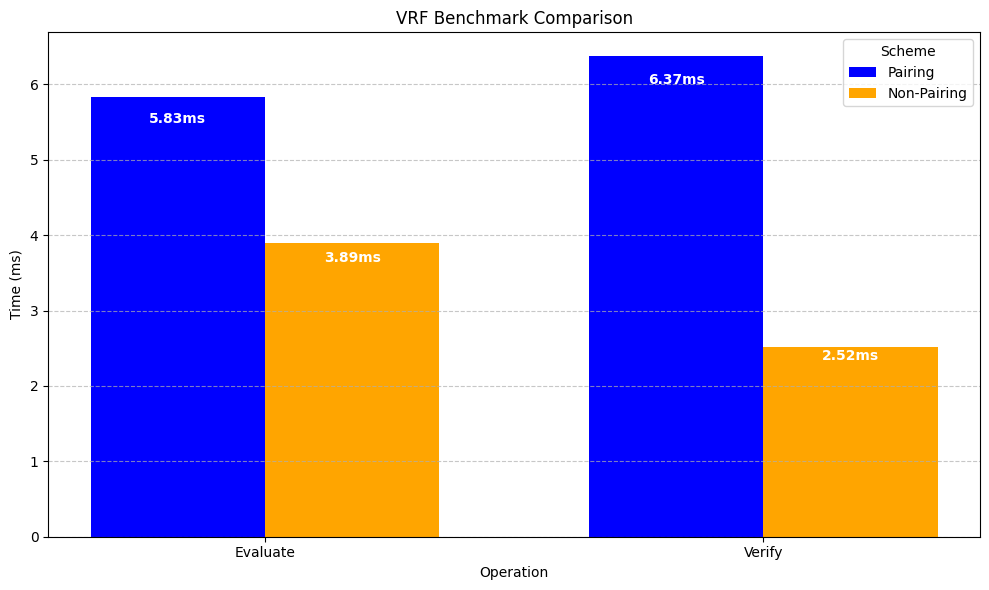
\includegraphics[width=0.75\linewidth]{figures/vrf-benchmark.png}
    \caption{VRF Benchmark}
    \label{fig:vrf-benchmark}
\end{figure}


Include benchmark of my construction on a different curve e.g. secpk251
Try to benchmark it against a VRF from the standardisation






% \subsection{CRBN Instantiation In Identity System}

% The Credential Relationship Binding Nullifier (CRBN) extends the Multi-Issuer Multi-Credential Anonymous Credential (MIMC-ABC) system from Chapter 3 to support a hierarchical structure with sybil resistance. We define two credential types: a \emph{Master Credential} containing a secret key $\k$, and \emph{Context Credentials} with context identifiers $\ctx$. A nullifier $\nul = g^{1/(\k + \ctx)} \in \G$ binds each Context Credential to the Master Credential, ensuring uniqueness per context while preserving privacy via zero-knowledge proofs.

% We modify MIMC-ABC’s algorithms as follows, reusing its position-binding Pedersen commitments and $\Sigma$-protocols. Let $\mathsf{pp}$ include $\G$, $p$, $g$, and commitment generators $(g_1, g_2, g_3, g_4, g)$, where $\ell = 4$ supports attributes $[\id, \ctx, \exp, \k]$ (extensible to more).

% \begin{itemize}
%     \item \textbf{Master Credential Issuance}:
%     \begin{itemize}
%         \item \emph{User}: Samples $\k \sample \Z_p$ and $\usk_m \sample \Z_p$. Computes commitment $\cmm = g_1^\id g_2^{\ctx_m} g_3^{\exp_m} g_4^\k g^{\usk_m}$, where $\ctx_m = \mathcal{H}(\text{"master"})$ and $\exp_m$ is the expiration. Runs $\mathsf{Obtain}(\attrs_m = [\id, \ctx_m, \exp_m, \k], \{\mathsf{opk}_j\}, \usk_m)$ with issuer $j_m$, proving $\cmm$’s opening via $\pircom$ (Section 2.4.3).
%         \item \emph{Issuer $j_m$}: Verifies the proof, signs $\sigma_m = \mathsf{RS.Sign}(\cmm, \mathsf{osk}_{j_m})$, and returns $\credm = (\sigma_m, \cmm)$ via $\mathsf{Issue}$.
%     \end{itemize}

%     \item \textbf{Context Credential Issuance}:
%     \begin{itemize}
%         \item \emph{User}: For context $\ctx_c$ (e.g., $\mathcal{H}(\text{"DMV"})$), samples $\usk_c \sample \Z_p$. Computes $\cmc = g_1^\id g_2^{\ctx_c} g_3^{\exp_c} g^{\usk_c}$ (no $\k$ here, as it’s from $\credm$). Runs $\mathsf{Obtain}(\attrs_c = [\id, \ctx_c, \exp_c, 0], \{\mathsf{opk}_j\}, \usk_c)$ with issuer $j_c$, proving $\cmc$’s opening and that position 4 is 0.
%         \item \emph{Issuer $j_c$}: Verifies the proof, optionally checks a nullifier registry (see below), signs $\sigma_c = \mathsf{RS.Sign}(\cmc, \mathsf{osk}_{j_c})$, and returns $\credc = (\sigma_c, \cmc)$.
%     \end{itemize}

%     \item \textbf{Nullifier Generation}: Given $\credm$ with $\k$ and $\credc$ with $\ctx_c$, compute:
%     \[
%     \nul = g^{1/(\k + \ctx_c)} \in \G
%     \]
%     where $\k + \ctx_c$ is computed in $\Z_p$, and the inverse $1/(\k + \ctx_c)$ exists with overwhelming probability (as $p$ is prime).

%     \item \textbf{Presentation and Verification}:
%     \begin{itemize}
%         \item \emph{User}: Inputs $\credm$, $\credc$, $\usk_m$, $\usk_c$, and a predicate $\phi$ (e.g., $\ctx_c = \text{"DMV"} \land \exp_c > \text{today}$). Rerandomizes $\credm$ to $(\sigma_m', \cmm')$ and $\credc$ to $(\sigma_c', \cmc')$ using $\Delta_{r_m}, \Delta_{r_c}$ (Section 3.3). Computes $\nul = g^{1/(\k + \ctx_c)}$ and proves:
%         \[
%         \mathcal{R}_{\mathsf{vrf}} = \zkpok \left\{ 
%         (\cmm', \cmc', \nul), (\id, \ctx_m, \exp_m, \k, \usk_m', \ctx_c, \exp_c, \usk_c') 
%         \middle|
%         \begin{array}{l}
%         \cmm' = g_1^\id g_2^{\ctx_m} g_3^{\exp_m} g_4^\k g^{\usk_m'} \land \ctx_m = \mathcal{H}(\text{"master"}) \land \\
%         \mathsf{RS.Ver}(\sigma_m', \cmm', \mathsf{opk}_{j_m}) = 1 \land \\
%         \cmc' = g_1^\id g_2^{\ctx_c} g_3^{\exp_c} g^{\usk_c'} \land \\
%         \mathsf{RS.Ver}(\sigma_c', \cmc', \mathsf{opk}_{j_c}) = 1 \land \\
%         \nul = g^{1/(\k + \ctx_c)} \land \phi(\ctx_c, \exp_c) = 1
%         \end{array} 
%         \right\}
%         \]
%         where $\usk_m' = \usk_m + \Delta_{r_m}$, $\usk_c' = \usk_c + \Delta_{r_c}$. The proof uses the $\Sigma$-protocol from Section 4.x (to be detailed).
%         \item \emph{Verifier}: Checks $\pi$, $\sigma_m'$, $\sigma_c'$, and $\nul$ against $\mathsf{opk}_{j_m}$, $\mathsf{opk}_{j_c}$. Optionally queries a nullifier registry to ensure $\nul$ is unused for $\ctx_c$.
%     \end{itemize}
% \end{itemize}

% \textbf{Note on Revocation}: If $\credm$ is revoked (e.g., via a public revocation list for $\cmm$ or $\k$), verifiers can reject proofs involving $\nul$, as $\k$’s validity underpins $\mathcal{R}_{\mathsf{vrf}}$. Details are deferred to Section 4.y.

% \textbf{Note on Sybil Resistance}: Issuers or verifiers may maintain a context-specific nullifier registry. During issuance, users prove $\nul$’s correctness in zero-knowledge; issuers reject duplicates. Alternatively, verifiers check $\nul$’s uniqueness during presentation, balancing privacy and accountability (see Section 4.z).

% This construction leverages MIMC-ABC’s efficient $\Sigma$-protocols and avoids pairings, using only standard group operations in $\G$. The nullifier $\nul$ enforces hierarchical binding and sybil resistance, computed deterministically from $\k$ and $\ctx_c$.





% \begin{table}
% \begin{center}
% \caption{Comparison of our construction over previous work.}
% \label{tab:comparison-chap4}
% \begin{tabular}{l|ccccc}
% Features    									& 
% Sybil Resist.  & 
% Hierarchy & 
% Private & 
% Pairing-Free & 
% Predicate Proofs \\
% \hline
% CanDID \cite{maram2021candid}     				&
% \ding{51}     & 
% \ding{51} 	& 
% \ding{55}  &  
% -     & 
% \ding{55}		\\
% SyRA \cite{crites_syra_2024}     				& 
% \ding{51}    	& 
% \ding{51}     & 
% \ding{51}  &  
% \ding{51}     & 
% \ding{55}		\\
% S3ID \cite{rabaninejad_attribute-based_2024}  & 
% \ding{51}     & 
% \ding{51}    	& 
% \ding{55}  &  
% \ding{55}     & 
% \ding{55}		\\
% UTT               & 
% \ding{51}     & 
% \ding{51}    	& 
% \ding{51}  &  
% \ding{55}     & 
% \ding{51}		\\
% Chap3             & 
% \ding{55}     & 
% \ding{55}    	& 
% \ding{51}  &  
% \ding{55}     & 
% \ding{51}		\\
% Ours  										& 
% \ding{51}     & 
% \ding{51}    	& 
% \ding{51}  &  
% \ding{51}     & 
% \ding{51}		\\
% \end{tabular}
% \end{center}
% \vspace{1em}
% \footnotetext[1]{Predicate Proofs allow users to prove statements about their credentials privately}
% \footnotetext[2]{Efficient Token refers to optimization of token verification}
% \end{table}


\subsection*{Notation}
Inline with our Anonymous Credential scheme built and prior chapters, the secret key is $\k$, the VRF input is $\ctx$, the VRF output is $\nul$ and the proof $\pi$ proves the correctness of $\nul$ such that $(\nul, \pi) \gets \mathsf{VRF.Eval}(\k, \ctx)$. $\cm = \CMCom([\id,\ldots];\usk)$ is a commitment shorthand for commitment $g_1^\id \ldots g^\usk$. We use Type-3 Bilinear Pairings. Let $\G_1$, $\G_2$, and $\G_T$ be groups of prime order $p$, with generators $g \in \G_1$, $\tilde{g} \in \G_2$, and a bilinear map $e: \G_1 \times \G_2 \to \G_T$.


\section{On the possibility of Sigma protocols for VRF Construction}
Why $\Sigma$-Protocols Suit Our VRF Construction

In our Verifiable Random Function (VRF) construction, we employ a $\Sigma$-protocol to generate the proof $\pi$ for the output $y = f_{sk}(x)$, where $sk$ is the secret key and $x$ is the input. A potential concern is whether the zero-knowledge property of $\Sigma$-protocols, which allows proof simulation, compromises the \textbf{verifiable uniqueness} property of the VRF—i.e., the guarantee that only one $y$ can be verified for a given $x$. Here, we explain why this concern is unfounded and how $\Sigma$-protocols align with VRF security requirements.

A VRF must satisfy three core properties: \textbf{correctness}, \textbf{uniqueness}, and \textbf{pseudorandomness}. \textbf{Correctness} ensures that an honestly computed output $y = f_{sk}(x)$ and its proof $\pi$ will always pass verification. \textbf{Uniqueness} guarantees that for each $x$, only one $y$ can be successfully verified with a proof $\pi$. \textbf{Pseudorandomness} ensures that without $sk$, $y$ is indistinguishable from random, even after seeing other $(x, y, \pi)$ triples. The $\Sigma$-protocol, an interactive proof system, offers three key properties: \textbf{completeness} (an honest prover with $sk$ convinces the verifier), \textbf{soundness} (a dishonest prover cannot prove a false statement), and \textbf{zero-knowledge} (the proof reveals nothing about $sk$, and a simulator can mimic it for true statements). These align perfectly with the VRF's needs: completeness supports correctness, soundness enforces uniqueness, and zero-knowledge preserves pseudorandomness by hiding $sk$.

The zero-knowledge property ensures $sk$ remains secret, but the simulator can only generate valid proofs for \textbf{true statements}, e.g., $y = f_{sk}(x)$. It cannot produce a proof for a false statement, like $y' \neq f_{sk}(x)$, that passes verification, due to the \textbf{soundness} property. Soundness ensures that only proofs for the correct $y$ are accepted, preventing an adversary from forging a proof for an incorrect output. Thus, the uniqueness of $y$ is preserved, as false proofs are rejected with overwhelming probability.

\textbf{Concrete Example:} Consider a VRF where $y = g^{1/(sk + x)}$ in a group of prime order $p$, and the $\Sigma$-protocol proves $y^{sk + x} = g$. Here, $y$ is uniquely determined by $sk$ and $x$ (since exponentiation is injective for $sk + x \neq 0 \mod p$). The $\Sigma$-protocol ensures that only the correct $y$ satisfies the equation, and a proof for an incorrect $y'$ (where $y'^{sk + x} \neq g$) fails verification. Despite zero-knowledge allowing simulation for the true $y$, soundness prevents valid proofs for false $y'$, reinforcing uniqueness.

A potential concern with using zero-knowledge proofs for VRFs is that proof simulatability might conflict with output uniqueness. In general NIZKs, the simulation property could potentially allow valid proofs for multiple outputs of the same input, e.g. $y_1, y_2$ for the same input $x$, violating the VRF uniqueness requirement. Our construction resolves this tension by leveraging a $\Sigma$-protocol to prove the statement $y^{sk + x} = g$ where $y = g^{1/(sk + x)}$. This equation has exactly one solution for $y$ given fixed values of $sk$ and $x$ (when $sk + x \neq 0 \mod p$). While the protocol's zero-knowledge property conceals $sk$, its soundness guarantees that only proofs for the correct $y$ will verify, thereby enforcing rather than compromising uniqueness.


In conclusion, the zero-knowledge property of $\Sigma$-protocols does not weaken the VRF's verifiable uniqueness, as simulation is limited to true statements. Meanwhile, soundness upholds the integrity of the proof, ensuring only the correct $y$ verifies.
  The impossibility of a VRF with with sigma protocol for proof.

  \mychapter{Threshold Sybil-Resistant Identity System}\label{chap6}

\section{Introduction}\label{sec:threshold-intro}
Self-sovereign identity (SSI) systems enable users to control their digital identities with strong privacy, Sybil resistance, and minimal issuer interaction. Distributing trust across multiple issuers is critical to avoid single points of failure. CanDID~\cite{maram2021candid} is a pioneering SSI system that uses multi-party computation (MPC) to deduplicate identities and issue credentials via a (threshold) committee of signing nodes. While effective, it has drawbacks: slow MPC-based deduplication, frequent issuer interactions, linkability risks, and little protection for credential non-transferability. Similar to Coconut~\cite{sonnino_coconut_2020}, a threshold credential system that distributes trust across multiple issuers, T-SIRIS employs a $t$-out-of-$N$ threshold issuance model to enhance decentralization. However, Coconut lacks a mechanism to prevent sybil attacks, a critical requirement for self-sovereign identity (SSI) systems. T-SIRIS addresses this gap by integrating anonymous, deterministic nullifiers from our Credential Relationship Binding Nullifier (CRBN) scheme (Chapter~\ref{chap4}), adding just 2.49ms to issuance overhead to credential issuance (Section~\ref{sec:threshold-performance}) while ensuring users cannot obtain multiple credentials per context.

This chapter presents T-SIRIS, a threshold Sybil-resistant identity system built on our multi-issuer multi-credential anonymous credential system (MIMC-ABC) from Chapter~\ref{chap3} and Credential Relationship Binding Nullifier (CRBN) from Chapter~\ref{chap4}. T-SIRIS uses a $t$-out-of-$N$ threshold issuance model, secure against $t-1$ malicious issuers. We compare T-SIRIS with CanDID and S3ID~\cite{rabaninejad_attribute-based_2024}, which uses threshold anonymous counting tokens (tACT), showing improvements in efficiency and functionality.


\subsection*{Chapter Roadmap}
% The remainder of the chapter is structured as follows: In Section \ref{sec-vrf-introduction} we introduce nullifiers and their role in privacy-preserving protocols. In Section \ref{sec-vrf-preliminaries}, we introduce the preliminaries and building blocks, in Section \ref{subsec:deterministic-nullifier}, we present our Prime Order DY VRF construction, followed by privacy-preserving extensions in Section \ref{sec:privacy-preserving-vrf}. In Section \ref{sec:performance-vrf}, we evaluate our performance against the state-of-the-art schemes, and in Section \ref{sec-vrf-instantiation}, we outline instantiations of our construction for Anonymous Credentials. 

\subsection{Motivation and Challenges}

Traditional Attribute-Based Anonymous Credential systems (ABCs) are based on a centralized issuer, which has its own security flaws - a malicious issuer can issue credentials that can't be traced in an anonymous system, undermining the system's integrity. To address this, we distribute security among $N$ nodes, requiring a threshold of at least $t$ nodes to issue a valid credential. 

Existing systems struggle to balance privacy, efficiency, and functionality. 

CanDID~\cite{maram2021candid} pioneered Sybil-resistant identity with legacy credential oracles, but relies on costly multi-party computation (MPC) among committee nodes for deduplication and requires interactive issuance for context credentials, contradicting self-sovereign principles. Each transaction requires communication with committee members, introducing privacy vulnerabilities where a single malicious node can link different user transactions.

\subsubsection*{CanDID}
CanDID deduplicates a user attribute, e.g. social security number using MPC, storing a unique value in a table $T_{\text{Dedup}}$. Users create a master credential from legacy data via oracles, then request context-specific credentials. Its limitations include:

\begin{itemize}
    \item \textbf{Deduplication:} MPC deduplication is slow and reveals a pseudonym to issuers, enabling pseudonym linking. T-SIRIS uses CRBN, computing a nullifier $y = g^{1/(k + \text{ctx})} \in \mathbb{G}_1$ with user key $k \in \mathbb{Z}_p$ and context $\text{ctx}$. This is anonymous and many times faster than tACT~\cite{rabaninejad_attribute-based_2024} (see Section~\ref{sec:perf}).

    \item \textbf{Efficient Deduplication and Verification:} T-SIRIS achieves fast deduplication using CRBN, computing a nullifier $y = g^{1/(k + \text{ctx})} \in \mathbb{G}_1$ with user key $k \in \mathbb{Z}_p$ and context $\text{ctx}$. Unlike Coconut~\cite{sonnino_coconut_2020}, which lacks sybil resistance, and CanDID’s MPC-based deduplication, CRBN is pairing-free and $5\times$ faster than S3ID’s tACT~\cite{rabaninejad_attribute-based_2024}. Verification scales sublinearly with attributes $n$, achieving up to $44.1\times$ speedup over tACT for $n=64$ (see Section~\ref{sec:perf}).
    
    \item \textbf{Context Credential Issuance:} CanDID requires issuer interaction for each context credential, e.g., ``over 18.’’ T-SIRIS users receive credentials from different issuers and use ZKPs to prove predicates $\phi(\vec{m}) = m_1 \geq 18$ based on the attributes in their set of credentials, allowing flexibility and dynamic verification scenarios without interacting with an issuer each time. 
    
    \item \textbf{Sybil Resistance:} CanDID tracks public keys, risking linkability. T-SIRIS embeds $k$ in all credentials, using CRBN with ZKP $\Pi^{\mathcal{R}_{\text{null}}} = \text{ZKPoK}\{(k): y = g^{1/(k + \text{ctx})}\}$ for unlinkable Sybil resistance.
\end{itemize}

Both systems use a master-context credential hierarchy, but T-SIRIS allows different issuers for context credentials and supports flexible ZKP-based predicates.

\subsubsection*{S3ID/tACT} \cite{rabaninejad_attribute-based_2024} uses tACT, based on Shacham-Waters signatures, for Sybil resistance and threshold issuance. Both T-SIRIS and S3ID embed a user key $k$ in credentials. T-SIRIS improves in:
\begin{itemize}
    \item \textbf{Efficiency:} CRBN and Schnorr ZKPs avoid pairings, offering up to $44.1\times$ faster verification for $n=64$ attributes (see Section~\ref{sec:perf}).
    \item \textbf{Predicate Support:} S3ID’s Groth-Sahai proofs limit predicate expressiveness. T-SIRIS’s MIMC-ABC supports complex computation over group exponents e.g. Schnorr proofs and Range Proofs (see Chapter~\ref{chap:proofs}).
\end{itemize}

\subsubsection*{Oracle Integration}


\subsubsection*{Managing SSI Features with Privacy Preserving Cryptography}
SSI requires unlinkability, Sybil resistance, and efficiency. Approaches include tokens (tACT~\cite{rabaninejad_attribute-based_2024}), zkSNARKs~\cite{rosenberg_zk-creds_2022}, and anonymous credentials (ABC). T-SIRIS’s ABC-based design with CRBN and MIMC-ABC balances speed and flexibility, scaling well with attributes $n$ and issuers $N$.


\subsection{Contributions}
\label{sec:tsiris_contributions}

Our Threshold Sybil-Resistant Identity System (T-SIRIS) advances self-sovereign identity (SSI) by combining efficiency, expressiveness, and security in a multi-issuer setting. Built on the Multi-Issuer Multi-Credential Anonymous Credential system (MIMC-ABC) from Chapter~\ref{chap3} and the Credential Relationship Binding Nullifier (CRBN) from Chapter~\ref{chap4}, T-SIRIS outperforms existing systems like CanDID~\cite{maram2021candid} and S3ID~\cite{rabaninejad_attribute-based_2024}. Below, we outline our contributions, aligning them with S3ID’s claims to highlight T-SIRIS’s improvements.

\begin{enumerate}
    \item \textbf{Efficient Deduplication and Verification:} T-SIRIS achieves fast deduplication using CRBN, computing a nullifier $y = g^{1/(k + \text{ctx})} \in \mathbb{G}_1$ with user key $k \in \mathbb{Z}_p$ and context $\text{ctx}$. Unlike Coconut~\cite{sonnino_coconut_2020}, which lacks sybil resistance, and CanDID’s MPC-based deduplication, CRBN is pairing-free and many times faster than S3ID’s tACT~\cite{rabaninejad_attribute-based_2024}. Verification scales sublinearly with attributes $n$, achieving up to $44.1\times$ speedup over tACT for $n=64$ (see Section~\ref{sec:perf}).
    
    \item \textbf{Expressive Predicate Proofs:} T-SIRIS supports complex predicates (e.g., $\phi(\vec{m}) = m_1 \geq 18 \wedge m_2 \in S$) via MIMC-ABC and Schnorr-based zero-knowledge proofs (ZKPs). Unlike S3ID’s Groth-Sahai proofs, which limit expressiveness, T-SIRIS enables range proofs and set membership with sublinear complexity, enhancing flexibility for SSI applications (see Chapter~\ref{chap6}).
    
    \item \textbf{Provably Secure Multi-issuer SSI:} T-SIRIS provides formal security definitions and proofs for unforgeability, Sybil resistance, strong unlinkability, and identity binding, secure against $t-1$ malicious issuers in a $t$-out-of-$N$ threshold model. Our proofs, based on the $q$-DDHI assumption for CRBN and SDLP for MIMC-ABC, extend S3ID’s tACT-based security to multi-issuer settings with identity binding (see Section~\ref{sec:security}).
    
    \item \textbf{Non-transferability and Identity Binding:} T-SIRIS embeds a user key $k$ in all credentials, ensuring only the owner can use them, similar to S3ID. Additionally, MIMC-ABC binds credentials from multiple issuers to a single identifier $\text{id} \in \mathbb{Z}_p$, enabling proofs of shared identity without revealing it. This strengthens S3ID’s non-transferability by supporting multi-issuer scenarios (see Section~\ref{sec:construction}).
\end{enumerate}

\textbf{Comparison with S3ID/tACT:} S3ID~\cite{rabaninejad_attribute-based_2024} claims efficient deduplication, non-interactive credential generation, unlinkability, and non-transferability using tACT. T-SIRIS achieves these with superior efficiency (CRBN vs. tACT) and expressiveness (Schnorr vs. Groth-Sahai). While S3ID supports single-issuer deduplication, T-SIRIS’s MIMC-ABC enables multi-issuer identity binding, addressing a broader range of SSI use cases. Both systems ensure non-transferability via a private key, but T-SIRIS’s ZKP $\Pi^{\mathcal{R}_{\text{null}}} = \text{ZKPoK}\{(k): y = g^{1/(k + \text{ctx})}\}$ offers stronger unlinkability against colluding issuers.


\begin{table}[ht]
\centering
\caption{Comparison of T-SIRIS with prior SSI systems.}
\label{tab:comparison-chap5}
\begin{tabular}{l|cccccc}
\toprule
\textbf{System} & \textbf{Sybil Resist.} & \textbf{Threshold} & \textbf{Non-Interact.}$^{\dagger}$ & \textbf{Non-Transfer.}$^{\ddagger}$ & \textbf{Complex Pred.}$^{\S}$ & \textbf{M.I. Anon.}$^{\P}$ \\
\midrule
CanDID~\cite{maram2021candid} & \ding{51}$^{\text{a}}$ & \ding{51} & \ding{55} & \ding{55} & \ding{55} & \ding{55} \\
SyRA~\cite{crites_syra_2024} & \ding{51} & \ding{55} & \ding{51} & \ding{55} & \ding{55} & \ding{55} \\
S3ID~\cite{rabaninejad_attribute-based_2024} & \ding{51} & \ding{51} & \ding{51} & \ding{51} & \ding{55} & \ding{55} \\
Coconut~\cite{sonnino_coconut_2020} & \ding{55} & \ding{51} & \ding{51} & \ding{55} & \ding{51} & \ding{55} \\
T-SIRIS (Ours) & \ding{51} & \ding{51} & \ding{51} & \ding{51} & \ding{51} & \ding{51} \\
\bottomrule
\end{tabular}
\begin{flushleft}
\footnotesize
$^{\dagger}$ Non-interactive application credential generation (Section~\ref{sec:construction}). \\
$^{\ddagger}$ Credentials bound to the true owner (Section~\ref{sec:construction}). \\
$^{\S}$ Support for complex predicates, e.g., range proofs (Section~\ref{sec:proofs}). \\
$^{\P}$ Anonymity against malicious issuers (Section~\ref{sec:security}). \\
$^{\text{a}}$ Pseudonymous, not fully anonymous. \\
\textit{Note:} We compare with CanDID for its SSI prominence, SyRA for its VRF-based Sybil resistance, S3ID for its threshold similarity, and Coconut for its threshold issuance baseline.
\end{flushleft}
\end{table}







\section{Preliminaries}

\begin{definition}[Shamir Secret Sharing]
A $(t,n)$ secret sharing scheme $\mathsf{SS}$ consists of the following $\PPT$ algorithms over message space $\mathcal{X}$:
\begin{itemize}
    \item $\mathsf{Share}(1^{\lambda}, t, n, x) \to ([x]_1, \dots, [x]_n):$ Takes security parameter $\lambda$, threshold $t$, number of parties $n$, and secret $x \in X$. Outputs $n$ shares $([x]_1, \dots, [x]_n)$.
    
    \item $\mathsf{Combine}([x]_{i_1}, \dots, [x]_{i_t}) \to x:$ Takes as input $t$ distinct shares $[x]_{i_j}$ where $i_j \in [n]$ for $j \in [t]$, and outputs the reconstructed secret $x \in \mathcal{X}$.
\end{itemize}
\end{definition}




\begin{definition}[Distributed Key Generation]
A $(t,n)$-Distributed Key Generation (DKG) protocol $\mathsf{DKG}$ for discrete-log based cryptosystems is an interactive $\PPT$ protocol executed by $n$ parties over a group $G$ with generator $g$, taking as input a security parameter $1^\lambda$, threshold $t$, and number of parties $n$. At completion, each honest party $P_i$ outputs:
\begin{itemize}
    \item A share $[x]_i \in \mathbb{Z}_q$ of a secret $x \in \mathbb{Z}_q$.
    \item A public key $y = g^x \in G$.
\end{itemize}
The protocol satisfies:
\begin{itemize}
    \item \textbf{Correctness:} All honest parties output the same $y$, and the shares $([x]_1, \dots, [x]_n)$ held by honest parties form a $(t,n)$-threshold sharing of $x$ such that $y = g^x$.
    \item \textbf{Uniformity:} The secret $x$ is uniformly distributed in $\mathbb{Z}_q$.
    \item \textbf{Security:} Against a static adversary corrupting up to $t < n/2$ parties, no information about $x$ is leaked beyond $y$, and correctness holds.
\end{itemize}
\end{definition}



\subsubsection{DKG Construction}
The $(t,n)$-DKG protocol from \cite{Gennaro2007} operates over a group $G$ with generator $g$, order $q$, and security parameter $\lambda = \log q$, executed by $n$ parties $P_1, \dots, P_n$ with threshold $t < n/2$. It proceeds in two phases:
\begin{itemize}
    \item \textbf{Phase 1 (Commitment):} Each party $P_i$:
        \begin{enumerate}
            \item Chooses a random secret $z_i \in \mathbb{Z}_q$ and a polynomial $f_i(z)$ of degree $t$ with $f_i(0) = z_i$.
            \item Uses Pedersen’s VSS to distribute verifiable shares $s_{ij} = f_i(j)$ and commitments $C_{ik} = g^{a_{ik}} h^{b_{ik}}$ (for coefficients $a_{ik}$, blinding $b_{ik}$, and generator $h \in G$) to all parties $P_j$.
            \item Verifies received shares $s_{ji}$ from others; if invalid, complains to disqualify the sender $P_j$. Let $QUAL$ be the set of non-disqualified parties.
        \end{enumerate}
    \item \textbf{Phase 2 (Key Generation):} Each party $P_i \in QUAL$:
        \begin{enumerate}
            \item Uses Feldman’s VSS to broadcast commitments $A_{ik} = g^{a_{ik}}$ for the same polynomial $f_i(z)$ from Phase 1.
            \item Verifies received commitments; if invalid, reconstructs $z_j$ of the faulty $P_j \in QUAL$.
            \item Computes share $[x]_i = \sum_{j \in QUAL} s_{ji}$ and public key $y = \prod_{j \in QUAL} A_{j0}$, where $A_{j0} = g^{z_j}$.
        \end{enumerate}
\end{itemize}
The protocol outputs $([x]_i, y)$ for each $P_i \in QUAL$, where $x = \sum_{j \in QUAL} z_j$ and $y = g^x$.


















\begin{definition}[Distributed Key Generation for VRF] 
A $(t,n)$-threshold DKG scheme consists of the following probabilistic polynomial-time algorithms:

\begin{itemize} 
\item $\mathsf{DistKeyGen}(1^{\lambda}, t, n) \to (\mathsf{pp}, \mathsf{vk}, \{[k_2]_i, \mathsf{vk}_i\}_{i \in [n]}):$ On input security parameter $\lambda$, threshold parameter $t < n$, and number of parties $n$, outputs public parameters $\mathsf{pp}$, a verification key $\mathsf{vk} = g^{k_2}$, and for each party $i$, a share $[k_2]_i$ of $k_2$ along with an individual verification key $\mathsf{vk}_i$.

\item $\mathsf{ShareProve}(\mathsf{pp}, [k_2]_i) \to \pi_i:$ Generates a proof $\pi_i$ that the share $[k_2]_i$ is valid.

\item $\mathsf{ShareVerify}(\mathsf{pp}, \mathsf{vk}_i, [k_2]_i, \pi_i) \to \{0,1\}:$ Verifies that a share $[k_2]_i$ is valid with respect to verification key $\mathsf{vk}_i$ using proof $\pi_i$.

\item $\mathsf{Reconstruct}([k_2]_{i_1}, \dots, [k_2]_{i_{t+1}}) \to k_2:$ Takes $t+1$ distinct valid shares and reconstructs the secret $k_2$.
\end{itemize}

The scheme satisfies the following security properties:

\begin{itemize}
\item \textbf{Correctness:} For any $(\mathsf{pp}, \mathsf{vk}, \{[k_2]_i, \mathsf{vk}_i\}_{i \in [n]}) \leftarrow \mathsf{DistKeyGen}(1^{\lambda}, t, n)$, any subset $S \subset [n]$ of size $|S| = t+1$, and $k_2 \leftarrow \mathsf{Reconstruct}(\{[k_2]_i\}_{i \in S})$, it holds that $\mathsf{vk} = g^{k_2}$.

\item \textbf{Secrecy:} Any adversary corrupting up to $t$ parties learns no information about $k_2$ beyond what can be derived from the verification key $\mathsf{vk}$.

\item \textbf{Robustness:} Even if up to $t$ parties behave maliciously, the honest parties can still successfully generate and verify shares.
\end{itemize}
\end{definition}



\begin{definition}[Distributed Key Generation]
A $(t,n)$-threshold Simple DKG scheme consists of the following algorithms:
\begin{itemize}
\item $\mathsf{Setup}(1^{\lambda}) \to \mathsf{pp}$: Outputs public parameters $\mathsf{pp} = (G, p, g)$ where $G$ is a cyclic group of prime order $p$ with generator $g$.
\item $\mathsf{DistKeyGen}(1^{\lambda}, t, n) \to (\mathsf{vk}, \{[k]_i, \mathsf{vk}_i\}_{i \in [n]})$: Generates a verification key $\mathsf{vk} = g^k$ and for each party $i$, a share $[k]_i$ of the secret key $k$ along with verification key $\mathsf{vk}_i = g^{[k]_i}$.
\item $\mathsf{ShareVerify}(\mathsf{pp}, \mathsf{vk}_i, [k]_i) \to \{0,1\}$: Verifies that share $[k]_i$ is consistent with verification key $\mathsf{vk}_i$.
\item $\mathsf{Reconstruct}(\{[k]_{i_j}\}_{j=1}^{t+1}) \to k$: Reconstructs the secret key $k$ from $t+1$ valid shares.
\end{itemize}
\end{definition}


Our Simple DKG scheme is defined as follows:
\begin{definition}[Simple Distributed Key Generation]
A $(t,n)$-threshold Simple DKG scheme consists of the following algorithms:
\begin{itemize}
\item $\mathsf{Setup}(1^{\lambda}) \to \mathsf{pp}$: 
  Outputs public parameters $\mathsf{pp} = (G, p, g)$ where $G$ is a cyclic group of prime order $p$ with generator $g$.
  
\item $\mathsf{DistKeyGen}(1^{\lambda}, t, n) \to (\mathsf{vk}, \{[k]_i, \mathsf{vk}_i\}_{i \in [n]})$: 
  Executes the distributed key generation process:
  \begin{enumerate}
    \item All $n$ parties jointly generate a secret key $k$ such that any subset of $t+1$ parties can reconstruct $k$.
    \item Outputs the global verification key $\mathsf{vk} = g^k$.
    \item Each party $i$ receives:
      \begin{itemize}
        \item A share $[k]_i$ of the secret key $k$, and
        \item A verification key $\mathsf{vk}_i = g^{[k]_i}$ to verify its share.
      \end{itemize}
  \end{enumerate}

\item $\mathsf{ShareVerify}(\mathsf{pp}, \mathsf{vk}_i, [k]_i) \to \{0,1\}$: 
  Verifies that the share $[k]_i$ held by party $i$ is consistent with its verification key $\mathsf{vk}_i$.
  \begin{itemize}
    \item Returns $1$ if the verification is successful (i.e., $[k]_i$ is valid).
    \item Returns $0$ otherwise.
  \end{itemize}

\item $\mathsf{Reconstruct}(\{[k]_{i_j}\}_{j=1}^{t+1}) \to k$: 
  Reconstructs the secret key $k$ using a subset of $t+1$ valid shares $\{[k]_{i_j}\}_{j=1}^{t+1}$. 
  \begin{itemize}
    \item Applies Lagrange interpolation over the valid shares to compute $k$.
    \item Outputs the reconstructed secret key $k$.
  \end{itemize}
\end{itemize}
\end{definition}

\begin{theorem}[Security Properties]
The Simple DKG construction satisfies the following properties:
\begin{itemize}
\item \textbf{Correctness}: For any execution of $\mathsf{DistKeyGen}$ producing shares $\{[k]_i\}_{i \in [n]}$, any subset $S \subset [n]$ of size $|S| = t+1$, and $k' \leftarrow \mathsf{Reconstruct}(\{[k]_i\}_{i \in S})$, it holds that $g^{k'} = \mathsf{vk}$.
\item \textbf{Secrecy}: Any adversary controlling at most $t$ parties learns no information about the secret key $k$ beyond what can be derived from the public verification keys.
\item \textbf{Binding}: It is computationally infeasible for an adversary to produce a valid share $[k]_i$ that is inconsistent with the verification key $\mathsf{vk}_i$.
\end{itemize}
\end{theorem}





\section{Threshold Rerandomizable Signature for ABCs}
\label{sec:threshold-construction}

We adopt the threshold PS signature scheme from \cite{tomescu2022utt} using Shamir secret sharing with similarities to \cite{sonnino_coconut_2020} to distribute trust among multiple issuers. The key pair $(\mathsf{sk}, \mathsf{vk})$ is $(t,n)$-secret-shared among the signers, where each signer $i$ holds a share secret key $\mathsf{sk}_i$ and a share verification key $\mathsf{vk}_i$. This enables subsets of at least $t+1$ signers to collaboratively produce a signature that verifies under the combined verification key $\mathsf{vk}$, while ensuring that no subset of $t$ or fewer signers can forge signatures.


\subsection{Overview}
We assume up to $t-1$ malicious issuers in an $n$-issuer system, where $t$ is the threshold, reflecting realistic collusion scenarios in decentralized settings. The adversary cannot break the hard problems our schemes are built upon, and network conditions support standard threshold protocols. Similar to Coconut’s threshold issuance~\cite{sonnino_coconut_2020}, our threshold PS signature scheme distributes trust among $n$ issuers using Shamir secret sharing. However, we extend this foundation by integrating nullifiers from Chapter~\ref{chap4}, enabling sybil resistance—a critical feature for identity systems that Coconut does not address.

Importantly, this threshold construction distributed trust among multiple issuers while preserving the core properties of our underlying building block PS signature scheme - unforgeability and rerandomizability. Additionally, the end-signature algebraic structure is the same, and therefore, the verification algorithm and proof system compatibility are the same.
\subsection{Definition}

\begin{definition}[PS Threshold Signatures over Pedersen Commitments]
A PS threshold signature scheme $\mathsf{RS}$ over Pedersen commitments consists of the following algorithms:
\begin{itemize}
    \item $\mathsf{DistKeyGen}(1^{\lambda}, t+1, n, \ell) \to (\mathsf{ck}, \mathsf{vk}, (\mathsf{sk}_i, \mathsf{vk}_i)_{i \in [n]}):$ Takes security parameter $\lambda$, corruption threshold $t$, number of parties $n$, and attribute count $\ell$. Outputs commitment key $\mathsf{ck}$, verification key $\mathsf{vk}$, and per-party keys $(\mathsf{sk}_i, \mathsf{vk}_i)$.
    
    \item $\mathsf{ShareSign}(\mathsf{ck}, \mathsf{sk}_i, (\mathsf{cm}_k, \pi_k^{\mathsf{zkpok}})_{k \in [\ell]}; h) \to [\sigma^*]_i:$ Takes party $i$'s secret key $\mathsf{sk}_i$, commitments $\mathsf{cm}_k$ with ZK proofs $\pi_k^{\mathsf{zkpok}}$, and randomizer $h$. Outputs signature share $[\sigma^*]_i$.
    
    \item $\mathsf{ShareVer}(\mathsf{ck}, \mathsf{vk}_i, (\mathsf{cm}_k, \pi_k^{\mathsf{zkpok}})_{k \in [\ell]}, [\sigma^*]_i; h) \to \{0,1\}:$ Takes party $i$'s verification key $\mathsf{vk}_i$, commitments with proofs, and signature share $[\sigma^*]_i$. Outputs accept ($1$) or reject ($0$).
    
    \item $\mathsf{Aggregate}(\mathsf{ck}, \{[\sigma^*]_i\}_{i \in S}, \{r_k\}_{k \in [\ell]}) \to \sigma:$ Takes signature shares from subset $S$ of parties and commitment randomness values. Outputs aggregated signature $\sigma$.

    \item $\mathsf{Rerand}(\mathsf{vk}, \sigma, \Delta_r, \Delta_u) \rightarrow \sigma'$: Creates a rerandomized signature $\sigma'$ from signature $\sigma$ using randomization values $\Delta_r, \Delta_u$.
    
    \item $\mathsf{Verify}(\mathsf{vk}, \mathsf{cm}, \sigma) \rightarrow \{0,1\}$: Verifies signature $\sigma$ on commitment $\mathsf{cm}$ using public key $\mathsf{vk}$.
    
\end{itemize}
\end{definition}




\subsubsection{Construction}\label{threshold-ps-construction}


Our threshold PS construction works as follows:
A user with attributes $\attrs = [m_1, \ldots, m_\ell]$ generates a commitment $\cm = \CMCom([\attrs];r)$. The user interacts with signers using a pre-agreed random element $h \in \G_1$, alternatively, \cite{sonnino_coconut_2020} generates this with a hash-to-group of the commitment $h \gets \mathcal{H}(\cm)$. The user sends $\cm$ with $\Pi_{\cm}$ OR $\pi^{\mathsf{zkpok}}$ proving its opening to each signer. Signers verify the proof and return a signature share $[\sigma^*]_i = \mathsf{tPSutt.ShareSign}(\ck, \mathsf{sk}_i, (\mathsf{cm}_k, \pi^{\mathsf{zkpok}}); h)$. The user verifies each share and checks the consistency of the message and proof previously shared $\mathsf{tPSutt.ShareVer}(\ck, \mathsf{vk}_i, (\mathsf{cm}, \pi^{\mathsf{zkpok}}), [\sigma^*]_i; h)$. The user identifies a set $S$ of at least $t+1$ valid shares and aggregates them, outputting their signature $\sigma \leftarrow \mathsf{tPSutt.Aggregate}(\ck, ([\sigma^*]_i)_{i \in S}, r)$ which verifies under the combined  verification key $\mathsf{PSutt.Ver}(\mathsf{vk}, \mathsf{cm}, \sigma) = 1$.


\begin{itemize}
    \item $\mathsf{tDistKeyGen}(1^{\lambda}, t+1, n, \ell) \to (\ck, \vk, (\mathsf{sk}_i, \mathsf{vk}_i)_{i \in [n]}):$ Takes input the security parameter, $t$ the corruption threshold, $n$ is number of nodes, $\ell$ is the credential message length. Outputs $\ck, \vk$ the commitment and verification keys generated with the secrets and $\sk_i, \vk_i$ the shared keys to distribute to $n$ nodes. let $\mathcal{X}$ and $\psi_k $ be $t$ degree polynomials:
    \begin{itemize}
        \item For the shared $x$ values: $\mathcal{X} \sample \Z_p[X], x \gets \mathcal{X}(0)$, $\{[x]_i \gets \mathcal{X}(i)\}_{i\in [n]}$
        \item For the $k$ shared $y$ values: $\{\psi_k \sample \Z_p[X], y_k \gets \psi_k(0)\}_{k \in [\ell]}$, $\{[y_k]_i \gets \psi_k(i)\}_{k \in [\ell], i \in [n]}$
        \item using the secret, non-shared values, trusted setup party computes $\vk \gets \tilde{g}^x, \ck \gets \CMSetup(1^{\lambda}, \ell, \vec{y})$ and parses $\ck$ as $(g, \vec{g}, \tilde{g}, \vec{\tilde{g}})$. Note that $g_k = g^{y_k}, \tilde{g}_k = \tilde{g}^{y_k}$
        \item computes shared secret values $\{\sk_i \gets ([x]_i, ([y_k]_i))_{k\in[\ell]}\}_{i \in [n]}, \{\vk \gets (\tilde{g}^{[x]_i}, (\tilde{g}^{[y_k]_i})_{k\in[\ell]})\}_{i \in [n]}$
        \item $\mathsf{Return } $ $ \ck, \vk, \{\sk_i, \vk_i\}_{i \in [n]}$
    \end{itemize}
        

    \item $\mathsf{tShareSign}(\ck, \mathsf{sk}_i, \{\cm_k, \pi_k^{\mathsf{zkpok}}\}_{k \in [\ell]}, h) \to [\sigma^*]_i:$ the user runs $\mathsf{tShareSign}$ with at least $t$ nodes. 
    \begin{itemize}
        \item User commits to each $m$ individually: $\cm_k = h^{m_k}g^{r_k}$ and generates proofs for each $\cm_k = \zkpok(\cm_k, m_k, r_k)$ and sends each signer the commitment and proof.
        \item Signer parses $g$ from $\ck$ and verifies the opening of the commitment w.r.t. the proof.
        \item Signer parses $\sk_i$ as $[x]_i, \{[y_k]_i\}_{k \in [\ell]}$
        \item Signer signs their share $[\sigma^*]_i \gets (h, h^{[x]_i} \prod_{k \in [\ell]} \cm_k^{[y_k]_i} )$ = $(h, h^{[x]_i + \sum_{k \in [\ell]} m_k[y_k]_i} \cdot g^{\sum_{k \in [\ell]} r_k [y_k]_i})$
    \end{itemize}


    \item $\mathsf{tShareVer}(\ck, \mathsf{vk}_i, \{\cm_k, \pi_k^{\mathsf{zkpok}}\}_{k \in [\ell]}, [\sigma^*]_i; h) \to \{0,1\}:$ Run by a user to verify the signed share returned from each node before aggregating together. 
    \begin{itemize}
        \item Parse $[\sigma^*]_i$ as $([\sigma^*]_{i,1}, [\sigma^*]_{i,2})$ and check $h = [\sigma^*]_{i,1}$. 
        \item Verify each message commitment $\cm_k$ and proof $\pi_k$
        \item Parses $\vk_i$ as $(\tilde{g}^{[x]_i}, \{\tilde{g}^{[y_k]_i}\}_{k \in [\ell]})$
        \item Asserts $e([\sigma^*]_{i,2}, \tilde{g}) = e(h, \tilde{g}^{[x]_i}) \cdot \prod_{k \in [\ell]} e(\cm_k, \tilde{g}^{[y_k]_i})$
    \end{itemize}

    \item $\mathsf{tAggregate}(\ck, ([\sigma^*]_i)_{i \in S}, \{r_k\}_{k \in [\ell]}) \to \sigma:$ User parses $\ck$ as $(\cdot, \vec{g}, \cdot, \cdot)$ and $\forall i \in S$, parse $[\sigma^*]_i$ as $(h, [\sigma^*]_{i,2})$. Runs Lagrange Interpolation on $|S|=t+1$ signature shares:
    \begin{itemize}
        \item  $\mathcal{L}_i \gets \prod_{j \in S, j\neq i}\frac{0-j}{i-j} \forall i \in S$
        \item $\sigma_2 \gets \prod_{j \in S}([\sigma^*]_{i,2})^{\mathcal{L}_i}$ = 
        $(h, h^{x + \sum_{k \in [\ell]} m_ky_k} \cdot g^{\sum_{k \in [\ell]} r_ky_k})$ where $g_k = g^{y_k}$
        \item $\sigma \gets (h, \sigma_2 / \prod_{k \in [\ell]}g_k^{r_k})$ = $(h, h^{x + \sum_{k \in [\ell]}m_ky_k})$
    \end{itemize}

    \item $\mathsf{RS.Rerand}(\sigma, \Delta_r, \Delta_u) \to \sigma':$
        Parse $\sigma$ as $(\sigma_1, \sigma_2)$
        Set $\sigma_1' \gets \sigma_1^{\Delta_u}$
        Set $\sigma_2' \gets (\sigma_2 \cdot \sigma_1^{\Delta_r})^{\Delta_u}$
        Return $\sigma' \gets (\sigma_1', \sigma_2')$
    
    \item $\mathsf{RS.Ver}(\vk, \cm, \sigma) \to \bit:$
        Parse $\sigma$ as $(\sigma_1, \sigma_2)$, The prover $\Prover$ runs a Proof of Knowledge protocol with the following relation 
    \[
        \mathcal{R} \gets \mathsf{PoK}\{(m_1,\ldots,m_\ell, r + \Delta_r): 
    \]
    \[
         e(\sigma_2', \tilde{g}) = e(\sigma_1', \vk)\cdot e(\sigma_1', \widetilde{\cm}') \quad \wedge \quad
        e(\cm', \tilde{g}) = e(g, \widetilde{\cm}') \quad \wedge \quad
        \cm' = g^{r + \Delta_r} \prod_{i=1}^\ell g_i^{m_i}
        \}
    \]

\end{itemize}

\subsubsection{Security Properties}

The threshold PS signature scheme preserves the security of the underlying PS signature scheme while distributing trust across multiple parties.

\begin{theorem}[Threshold Unforgeability]
The scheme is unforgeable against adversaries corrupting up to $t-1$ signers, assuming the hardness of the Discrete Logarithm (DL) problem and the unforgeability of the PS signature scheme.
\end{theorem}

\begin{theorem}[Rerandomizability]
Signatures can be rerandomized to prevent linking, with the distribution of rerandomized signatures computationally indistinguishable from fresh signatures on the same message.
\end{theorem}

Formal proofs are omitted, as they follow from Shamir’s secret sharing security and the PS signature properties in Chapter~\ref{chap2}.






\section{T-SIRIS: Threshold Sybil-Resistant Identity System}
\label{sec:tsiris}
Building on our threshold PS signature scheme, we now present T-SIRIS, a complete threshold sybil-resistant identity system. T-SIRIS integrates threshold issuance, similar to Coconut~\cite{sonnino_coconut_2020}, with credential relationship binding nullifiers (Chapter~\ref{chap4}) to prevent sybil attacks (formalized in Definition [Sybil Resistance]), distinguishing it as a robust SSI solution. T-SIRIS integrates four key components:
\begin{itemize}
    \item \textbf{Threshold Key Generation}: Uses distributed key generation (DKG) with Shamir secret sharing for decentralized trust across $n$ issuers.
    \item \textbf{Threshold Issuance}: Extends MIMC-ABC (Chapter~\ref{chap3}) to issue credentials with $t$ of $n$ issuers, ensuring robustness.
    \item \textbf{Deduplication}: Employs nullifiers from Chapter~\ref{chap4} for efficient sybil resistance without costly operations.
    \item \textbf{Expressive Proofs}: Leverages Chapter~\ref{chap2}'s ABCs for privacy-preserving predicate verification (e.g., range proofs).
\end{itemize}


We assume up to $t-1$ malicious issuers in an $n$-issuer system, where $t$ is the threshold. These malicious issuers may:
\begin{itemize}
    \item Deviate from the protocol specification
    \item Collude to attempt to forge credentials
    \item Attempt to track or deanonymize users
    \item Refuse to participate in the issuance protocol
\end{itemize}

We also assume users may attempt sybil attacks by requesting multiple credentials for the same context. However, the adversary cannot break the underlying cryptographic assumptions (DL and $q$-DDHI).



\subsection{Definition}

A tSIRIS system consists of the following probabilistic polynomial-time (PPT) algorithms, parameterized by a security parameter $\lambda$ and attribute vector length $\ell$. We use $\RSSetup, \RSRand, \RSVer$ from the rerandomizable signature scheme.

\begin{definition}[tSIRIS]
    \begin{itemize}
    \item $\mathsf{RS.Setup}(1^\lambda) \to \mathsf{pp}$: Outputs public parameters $\mathsf{pp}$, including a bilinear group $\BG = (\G_1, \G_2, \G_T, e, g, \tilde{g}, p)$.

    \item $\mathsf{tKeyGen}(\mathsf{pp}, \ell, t, n) \to (\ck, \vk, \{(\mathsf{sk}_i, \mathsf{vk}_i)\}_{i \in [n]})$: Generates public commitment and verification keys  $\mathsf{ck}, \mathsf{vk}$ and distributes secret/verification key shares to $n$ issuers using a $(t,n)$-threshold scheme.

    \item $\mathsf{Dedup}(\credm, \cmc, \nullifier, \pi_{\nullifier}, \mathcal{T}) \to (\bit, T'):$ Takes input the user master credential $(\credm = \sigmam, \cmm, \uskm)$ and context commitment $\cmc$, the nullifier $\nullifier$ and its proof of correctness $\pi_{\nullifier}$ and the redeemed credential list $\mathcal{T}$. Outputs 0 if the proof fails or outputs 1 and updates the credential list T with $\nullifier$

    \item $(\mathsf{tObtainMaster}(\attrs, \ck, \{\mathsf{vk}_i\}_{i \in S}), \mathsf{tIssueMaster}(\{(\mathsf{sk}_i)\}_{i \in S}, \{\cm_k, \pi_k\}_{k \in [\ell]})) \to (\credm, \bot)$: an interactive protocol between a user running $\mathsf{tObtainMaster}$ from a subset $S$ of issuers where $|S| \geq t$ with each issuer running $\mathsf{tIssueMaster}$. $\mathsf{tObtainMaster}$ takes in the user's attributes $\attrs$, commitment key $\ck$ and verification key shares for at least $S$ nodes $\{\vk_i\}_{i \in S}$. $\mathsf{tIssueMaster}$ is run at least $|S|$ times, takes input the signers shared secret key $\sk_i$, commitment and proof pair for each message  $\{\cm_k, \pi_k\}_{k \in [\ell]}$. Outputs $\credm$ to the user and $\bot$ to itself.

    \item $(\mathsf{tObtainContext}(\credm, \attrs, \ck, \{\mathsf{vk}_i\}_{i \in S}), \mathsf{tIssueContext}(\{(\mathsf{sk}_i)\}_{i \in S}, \{\cm_k, \pi_k\}_{k \in [\ell]}, \aux)) \to (\credc, \bot)$: an interactive protocol between a user running $\mathsf{tObtainContext}$ from a subset $S$ of issuers where $|S| \geq t$ with each issuer running $\mathsf{tIssueContext}$.
    $\mathsf{tObtainContext}$ takes in the user's master credential $\credm$, new attributes $\attrs$, commitment key $\ck$ and verification key shares for at least $S$ nodes $\{\vk_i\}_{i \in S}$. $\mathsf{tIssueContext}$ is run at least $|S|$ times, takes input the signers shared secret key $\sk_i$, commitment and proof pair for each message  $\{\cm_k, \pi_k\}_{k \in [\ell]}$ and auxiliary information $\aux$ e.g. outputs $\nullifier, \pi_{\nullifier},\mathcal{T}$ from $\mathsf{Dedup}$ and $\credm, \pi_{\mathsf{verify}}$ from $\RSVer(\credm, \vk)$ for $\credm$. Outputs $\credc$ to the user and $\bot$ to itself.

    \item $(\mathsf{tShow}(\mathsf{cred}, \usk, \phi), \mathsf{Verify}(\mathsf{cred}', \pi)) \to \{0,1\}$: An interactive protocol between a user and verifier. The user inputs a credential $\cred = (\sigma, \cm, \usk)$ and predicate for verification $\phi$. $\mathsf{RS.Verify}$ takes input the rerandomized credential $\cred'$ and proof $\pi$ it satisfies $\phi$. The verifier outputs 1 if valid, 0 otherwise.
\end{itemize}
\end{definition}


\begin{definition}[Threshold Unforgeability]
Threshold Unforgeability captures that with $t-1$ corrupt issuers, an adversary cannot forge valid credentials. We define the following experiment:

$\textbf{Experiment}~\mathsf{Exp}^{\mathsf{unf}}_{\mathcal{A},\mathsf{T\text{-}SIRIS}}(\lambda):$
\begin{enumerate}
    \item $\mathsf{pp} \leftarrow \mathsf{Setup}(1^\lambda)$
    \item $(\mathsf{ck}, \mathsf{vk}, \{(\mathsf{sk}_i, \mathsf{vk}_i)\}_{i\in[n]}) \leftarrow \mathsf{KeyGen}(\mathsf{pp}, \ell, t, n)$
    \item Let $C$ be a set of corrupted issuers where $|C| \leq t-1$
    \item $\mathcal{A}$ is given $\{(\mathsf{sk}_i, \mathsf{vk}_i)\}_{i\in C}, \{\mathsf{vk}_i\}_{i\in[n]\setminus C}$
    \item $\mathcal{A}$ has access to credential issuance oracles $\mathcal{O}_{\text{obtain}},~\mathcal{O}_{\text{show}}$
    \item $\mathcal{A}$ outputs $(\mathsf{cred}', \phi, \pi)$
    \item The experiment returns 1 if:
    \begin{itemize}
        \item $\mathsf{Verify}(\mathsf{cred}', \phi, \pi) = 1$
        \item $\mathsf{cred}'$ was not legitimately issued to a corrupted user
        \item $\phi(\vec{m}) = 0$, where $\vec{m}$ are the attributes in $\mathsf{cred}'$
    \end{itemize}
\end{enumerate}

A T-SIRIS scheme satisfies threshold unforgeability if for any PPT adversary $\mathcal{A}$, there exists a negligible function $\mathsf{negl}$ such that:

$\Pr[\mathsf{Exp}^{\mathsf{unf}}_{\mathcal{A},\mathsf{T\text{-}SIRIS}}(\lambda) = 1] \leq \mathsf{negl}(\lambda)$
\end{definition}








\subsection{Sybil Resistance}

We formalize sybil resistance, capturing that no user can obtain multiple credentials for the same context, even when interacting with multiple (potentially corrupted) subsets of issuers:

\begin{definition}[Sybil Resistance]
We formalize sybil resistance as a user unable to obtain multiple credentials for the same context even when interacting with multiple (potentially corrupt) subset of issuers:

$\textbf{Experiment}~\mathsf{Exp}^{\mathsf{sybil}}_{\mathcal{A},\mathsf{T\text{-}SIRIS}}(\lambda):$
\begin{enumerate}
    \item $\mathsf{pp} \leftarrow \mathsf{Setup}(1^\lambda)$
    \item $(\mathsf{ck}, \mathsf{vk}, \{(\mathsf{sk}_i, \mathsf{vk}_i)\}_{i\in[n]}) \leftarrow \mathsf{KeyGen}(\mathsf{pp}, \ell, t, n)$
    \item Let $C$ be a set of corrupted issuers where $|C| \leq t-1$
    \item $\mathcal{A}$ is given $\{(\mathsf{sk}_i, \mathsf{vk}_i)\}_{i\in C}, \{\mathsf{vk}_i\}_{i\in[n]\setminus C}$
    \item Initialize deduplication table $\mathcal{T} = \emptyset$
    \item $\mathcal{A}$ interacts with credential issuance oracles
    \item $\mathcal{A}$ outputs master credential $\mathsf{cred}_{\text{master}}$, context $\mathsf{ctx}$ and two context credentials $(\mathsf{cred}_1, \mathsf{cred}_2)$
    \item The experiment returns 1 if:
    \begin{itemize}
        \item $\mathsf{Verify}(\mathsf{cred}_{\text{master}}, \phi_{\text{master}}, \pi_{\text{master}}) = 1$
        \item $\mathsf{Verify}(\mathsf{cred}_1, \phi_{\mathsf{ctx}}, \pi_1) = \mathsf{Verify}(\mathsf{cred}_2, \phi_{\mathsf{ctx}}, \pi_2) = 1$
        \item $\mathsf{cred}_1$ and $\mathsf{cred}_2$ have the same context $\mathsf{ctx}$
        \item $\mathsf{cred}_1$ and $\mathsf{cred}_2$ were issued using the same $\mathsf{cred}_{\text{master}}$
        \item $\mathsf{cred}_1 \neq \mathsf{cred}_2$ (i.e., they are distinct credentials)
    \end{itemize}
\end{enumerate}

A T-SIRIS scheme satisfies sybil resistance if for any PPT adversary $\mathcal{A}$, there exists a negligible function $\mathsf{negl}$ such that:

$\Pr[\mathsf{Exp}^{\mathsf{sybil}}_{\mathcal{A},\mathsf{T\text{-}SIRIS}}(\lambda) = 1] \leq \mathsf{negl}(\lambda)$
\end{definition}



\subsection{Threshold Anonymity}

We formalize threshold anonymity, capturing that credentials remain unlinkable and reveal nothing beyond what's explicitly proven, even when up to $t-1$ issuers are corrupted:

\begin{definition}[Threshold Anonymity]
We define the following experiment:

$\textbf{Experiment}~\mathsf{Exp}^{\mathsf{anon-b}}_{\mathcal{A},\mathsf{T\text{-}SIRIS}}(\lambda):$
\begin{enumerate}
    \item $\mathsf{pp} \leftarrow \mathsf{Setup}(1^\lambda)$
    \item $(\mathsf{ck}, \mathsf{vk}, \{(\mathsf{sk}_i, \mathsf{vk}_i)\}_{i\in[n]}) \leftarrow \mathsf{KeyGen}(\mathsf{pp}, \ell, t, n)$
    \item Let $C$ be a set of corrupted issuers where $|C| \leq t-1$
    \item $\mathcal{A}$ is given $\{(\mathsf{sk}_i, \mathsf{vk}_i)\}_{i\in C}, \{\mathsf{vk}_i\}_{i\in[n]\setminus C}$
    \item For $i \in \{0,1\}$:
    \begin{itemize}
        \item User $i$ obtains a master credential $\mathsf{cred}_{\text{master}}^i$ with attributes $\mathsf{attrs}_i$
        \item User $i$ obtains a context credential $\mathsf{cred}_{\mathsf{ctx}}^i$ for context $\mathsf{ctx}$
    \end{itemize}
    \item $\mathcal{A}$ outputs predicate $\phi$ such that $\phi(\mathsf{attrs}_0) = \phi(\mathsf{attrs}_1) = 1$
    \item $b \sample \{0,1\}$
    \item Generate $(\mathsf{cred}', \pi) \leftarrow \mathsf{Show}(\mathsf{cred}_{\mathsf{ctx}}^b, \mathsf{usk}_b, \phi)$
    \item $b' \leftarrow \mathcal{A}(\mathsf{cred}', \pi)$
    \item The experiment returns 1 if $b' = b$, otherwise 0
\end{enumerate}

A T-SIRIS scheme satisfies threshold anonymity if for any PPT adversary $\mathcal{A}$, there exists a negligible function $\mathsf{negl}$ such that:

$\left|\Pr[\mathsf{Exp}^{\mathsf{anon-1}}_{\mathcal{A},\mathsf{T\text{-}SIRIS}}(\lambda) = 1] - \Pr[\mathsf{Exp}^{\mathsf{anon-0}}_{\mathcal{A},\mathsf{T\text{-}SIRIS}}(\lambda) = 1]\right| \leq \mathsf{negl}(\lambda)$
\end{definition}











\subsection{Notes on Security Definitions}

These security definitions capture the unique challenges of the threshold setting:

\begin{enumerate}
    \item \textbf{Threshold Unforgeability}: Ensures that even with $t-1$ corrupted issuers, an adversary cannot forge credentials or prove false statements about them.

    \item \textbf{Sybil Resistance}: Guarantees that the nullifier-based deduplication mechanism works correctly even when interacting with different subsets of issuers, preventing users from obtaining multiple credentials for the same context.

    \item \textbf{Threshold Anonymity}: Ensures that credential presentations reveal nothing beyond the proven statement, even when up to $t-1$ issuers collude. This is stronger than standard anonymity since it must account for partial issuer corruption.
\end{enumerate}

The deduplication table $\mathcal{T}$ should be replicated across all issuers or maintained through a consensus protocol.


















\subsection{Construction}

\subsubsection{Overview}
T-SIRIS operates in two credential issuance phases: master credential issuance and context credential issuance. The master credential establishes the user's base identity with a secret key $\k$, while context credentials are bound to this master credential through nullifiers derived from $\k$ and a context $\mathsf{ctx}$. The nullifier mechanism prevents sybil attacks by ensuring users can obtain only one credential per context.

\subsubsection*{Similarites to Anonymous Payment Systems}


\subsubsection*{Registration}
Since we are optimizing for a private, accountable system, we make a small trade-off in privacy during Master Credential generation to satisfy the efficiency and private accountability requirements of an organization or government deploying this system today. We note that we can swap our methods for complete privacy using credential oracles like \cite{zhang_deco_2020, celi_distefano_2025, baldimtsi_zklogin_2024, ritzdorf_tls-n_2018} with a reduction in security and accountability.
During Master Credential registration, we enforce the user's Master Credential to be issued in a semi-trusted process where the user verifies their identity to the registration authority during its issuance. This enables Sybil resistance on the user identifier, stronger security for their VRF key $k$ discussed below \ref{t-siris:vrf-key-k-gen}, which is used to attach other credentials to it. The Registration Authority keeps track of user identities and can request their revocation from the Accountability Authority with techniques from \cite{damgard_balancing_2020}. At the end of registration, the user has a master credential $\credm = (\sigmam, \cmm, \vkm)$, including a rerandomizable, threshold-signature over commitment.

\subsubsection{Multi-Party Protocol for VRF Key Generation}\label{t-siris:vrf-key-k-gen}
The VRF key $k$ is embedded in the master credential and used to generate nullifiers for every context credential. Therefore, $k$ must be generated in a way that prevents the user from stealing someone else's $k$ and embedding it in their master credential (and therefore generating their nullifiers and abusing the system), as well as ensuring the issuers can't modify or create it maliciously to attempt to break anonymity later.
In the single issuer protocol, the user commits to their $k_1$, $\cm_1 = \CMCom([k_1];r)$\footnote{$\cm$ contains more than just the VRF key $\k$, we simplify in this explanation for brevity} and shares with the issuer along with a proof of its opening. Issuer verifies the proof and generates $k_2$, commits to it without randomness, $\cm_2 = \CMCom([k_2];0)$ and returns $\cm_2, k_2$ to the user. The user aggregates $\cm = \cm_1 \cdot \cm_2$ and computes $k = k_1 + k_2$ and now has a fully formed $\cm = \CMCom([k_1 + k_2];r)$.
We adjust slightly for the threshold scenario. 
The user computes $k_1$, $\cm_1 = \CMCom([k_1];r)$ and a proof of its opening.
The issuers runs DKG with a subset  $|S| \geq t$ of nodes to produce $\vk = g^{k_2}$ and each node computes shared $\{k_{2_i}\}_{i \in S}$ and shares with the user (For efficiency, the issuers can precompute these values in bulk and retain a pool to choose from $k_2$).
The user computes $k_2$ by combining $|S| \geq t$ with $\mathsf{DKG.Combine(\{k_{2_i}\}_{i \in S})}$, the user then computes $\cm = \CMCom([k_1 + k_2];r)$ and runs a sigma protocol to prove its correctness during credential generation. 
\[
\mathcal{R}: \left\{ 
(\cm_1, \cm, \vk),(k_1, k_2, k, r) 
\middle| 
\begin{array}{lcl}
    \cm_1 = \CMCom([k_1];r) \; \wedge \; \\
    \vk = g^{k_2} \; \wedge \; \\
    \cm = \CMCom([k_1 + k_2];r)
\end{array} \right\}
\]
The issuer learns the user's identity during registration but never learns the complete VRF key, maintaining user privacy while still enabling credential verification. 

\subsubsection*{Context Credential Issuance}
A context credential is linked to a master credential with the same committed identifier e.g., $\cmm = \CMCom([id,\ldots];r_1), \cmc = \CMCom([id, \ldots];r_2)$ kept secret during the issuance process.
A context credential issuer may be the same threshold committee, but may also be in the form of a credential oracle \cite{zhang_deco_2020, celi_distefano_2025, baldimtsi_zklogin_2024, ritzdorf_tls-n_2018}. The context credential issuance criteria will vary depending on their individual requirements; we represent this as the predicate $\phi$ that should be satisfied by the user during issuance. For example, perhaps a user successfully completed their driving test and should be issued a driving license. A user interacting with the DMV should first verify their master credential (e.g. they have a valid passport), The user also commits to their identifier $\cmc = \CMCom([id, \ctxc, \ldots]; r_c)$ and proves their $id$ is consistent between the two commitments. The user proves this relation:
\[
\mathcal{R}_{\phi}: \left\{ 
\begin{array}{l}
(\credm = (\sigmam, \cmm), \cmc), \\
(id, k, \ctxm, \ctxc, r_m, r_c) 
\end{array}
\middle| 
\begin{array}{lcl}
    \RSVer(\cmm, \vkm) = 1 \; \wedge \; \\
    \cmm = \CMCom([id, \ctxm, k, \ldots]; r_m) \; \wedge \ctxm = \texttt{"master"} \; \wedge \; \\
    \cmc = \CMCom([id, \ctxc, \ldots]; r_c) \; \wedge \ctxc = \texttt{"DMV"} \; \\
\end{array} \right\}
\]
The Context Credential issuer verifies the correctness of $\phi$ and runs their signing protocol over $\cmc$.

\subsubsection*{Sybil Resistance}
In the above scenario, the DMV is issuing 


\subsubsection*{Revocation}


\subsubsection*{Freshness}




\subsubsection*{Threshold Security}





\begin{figure}\label{threshold-construction-ABC}
    \caption{tABC System}
    \begin{center}
    \begin{tabular}{l@{\hspace{5em}}c@{\hspace{5em}}l}
    \multicolumn{3}{l}{$\underline{\mathsf{tOrgKeyGen}(1^{\lambda}, 1^\ell)}$ for attribute vector length $\ell$ and threshold parameters $n, t$} \\[1em]
    \multicolumn{3}{l}{$\BG = (\G_1, \G_2, \G_T, e, g, \tilg, p) \sample \BGGen(\secparam), \; (\ck, \vk, \{\sk_i, \vk_i\}_{i \in [\ell]}) \gets \mathsf{tDistKeyGen}(1^{\lambda}, t+1, n, \ell, \BG)$} \\[1em]
    \multicolumn{3}{l}{$\pcreturn \text{ public keys } (\ck, \vk). \text{ Each node receives their key share } (\sk_i, \vk_i)$} \\[1em]
    \multicolumn{3}{l}{$\underline{\mathsf{(Obtain, Issue)}}$:} \\[1em]
    \multicolumn{3}{l}{$\pirzero(\cmm) = \zkpok\{(\k_1,\uskm) \mid \cmm = g_1^0g_2^0g_3^0g_4^{\k_1}g^{\usk} \}$} \\[1em]
    $\underline{\mathsf{Obtain}(\opk)}$ && $\underline{\mathsf{Issue}(\pirzero, \cmm, \id, \ctx, \exp, \osk)}$ \\[1em]
    \multicolumn{3}{l}{$\k_1, \uskm \sample \Z_p\;, \cmm_1 = \CMCom([0,0,0,\k_1];\uskm)$} \\[1em]
     & $\xrightarrow{\;\; \pirzero(\cmm_1) \;\;}$ & If $\pirzero(\cmm_1)$ fails, return $\bot$ \\[1em]
     \multicolumn{3}{r}{$\{\k_2\}_{i \in t} \sample \Z_p, \cm_2 = \CMCom([\id,\ctx,\exp,\k_2];0)$ where $\ctx$="master"} \\[1em]
     \multicolumn{3}{r}{$\cm = \cm_1 + \cm_2 = \CMCom([\id,\ctx,\exp,\k_1 + \k_2];\usk)$} \\[1em]
    If $\RSVer(\sigma, \cm, \opk) = 0$, return $\bot$ & $\xleftarrow{\qquad \sigma, \cm, \k_2, \id, \ctx, \exp \qquad}$ & $u \sample \Z_p, \; \sigma \sample \RSSign(\cm, \osk, u)$ \\[1em]
    \multicolumn{3}{l}{\; Else, return $\cred = (\sigma, \cm, \usk, \opk)$} \\[1em]
    \multicolumn{3}{l}{$\underline{\mathsf{(Show, Verify)}}$ for credential $\cred$ and predicate $\phi$:} \\[1em]
    \multicolumn{3}{l}{$\Pi_\phi = \zkpok\{(\vec{m}, \usk') \mid \cm' = \CMCom(\vec{m}; \usk') \wedge \RSVer(\sigma', \cm', \opk) = 1 \wedge \phi(\vec{m}) = 1 \}$} \\[1em]
    $\underline{\mathsf{Show}(\cred)}$ && $\underline{\mathsf{Verify}(\sigma', \cm', \pi_\phi, \opk)}$ \\[1em]
    \multicolumn{3}{r}{Send empty access policy $\phi = \bot$} \\[0.5em]
    \multicolumn{3}{l}{Parse $\cred = (\sigma, \cm, \usk, \opk)$} \\[0.5em]
    \multicolumn{3}{l}{\quad Sample $\Delta_\usk, \Delta_u \sample \Z_p$} \\[1em]
    \multicolumn{3}{l}{\quad $\sigma' = \RSRand(\sigma, \Delta_\usk, \Delta_u)$} \\[1em]
    \multicolumn{3}{l}{\quad $\cm' = \CMRand(\cm, \Delta_\usk), \; \usk' = \usk + \Delta_\usk$} \\[1em]
    \multicolumn{3}{l}{\quad Compute $\Pi_\phi$} \\[1em]
    & $\xrightarrow{\sigma', \cm', \pi_\phi}$ & If $\pi_\phi$ fails, return 0, else 1 \\[1em]
    \end{tabular}
    \end{center}
\end{figure}


\begin{figure}
    \caption{T-ABC System with Master Credential and Nullifier}
    \begin{center}
    \begin{tabular}{l@{\hspace{5em}}c@{\hspace{5em}}l}
    \multicolumn{3}{l}{$\underline{\mathsf{T-OrgKeyGen}(1^{\lambda}, 1^\ell)}$ for attribute vector length $\ell$} \\[1em]
    \multicolumn{3}{l}{$\BG = (\G_1, \G_2, \G_T, e, g, \tilg, p) \sample \BGGen(\secparam), \; \mathsf{ck} \sample \mathsf{CM.Setup}(\BG, \secparam, \ell)$} \\[1em]
    \multicolumn{3}{l}{$\text{Assume threshold keys } (\sk_1, \dots, \sk_n), \vk \text{ are generated via DKG.}$} \\[1em]
    \multicolumn{3}{l}{$\text{Return } (\osk, \opk) = ((\sk_1, \dots, \sk_n), (\vk, \ck))$} \\[1em]

    \multicolumn{3}{l}{$\underline{\mathsf{(ObtainContext, IssueContext)}}$ for context credential:} \\[1em]
    \multicolumn{3}{l}{$\text{Assume user holds master credential } \cred_{\text{master}} = (\sigma_{\text{master}}, \cm_{\text{master}}, \usk_{\text{master}}, \opk)$} \\[1em]
    \multicolumn{3}{l}{$\pirverkey(\vk, \ck) = \zkpok\{(\vk, x) \mid \vk = \tilde{g}^x \}$} \\[1em]
    \multicolumn{3}{l}{$\pirnull(\cm_{\text{master}}, \mathsf{ctx}) = \zkpok\{(\k_{\text{master}}, \usk_{\text{master}}) \mid \cm_{\text{master}} = g_1^{\id} g_2^{\text{"master"}} g_3^{\exp} g_4^{\k_{\text{master}}} g^{\usk_{\text{master}}} \land y = g^{1/(\k_{\text{master}} + \mathsf{ctx})} \}$} \\[1em]

    $\underline{\mathsf{ObtainContext}(\credm, \cmc)}$ && $\underline{\mathsf{IssueContext}(\pirverkey, \pirnull, y, \cm_{\text{ctx}}, \osk)}$ \\[1em]
    & $\xleftarrow{\pirverkey(\vk, \ck)}$ & Each issuer $i$ sends $\pirverkey(\vk, \ck)$ \\[1em]
    If $\pirverkey(\vk, \ck)$ fails for any $i$, return $\bot$ && \\[1em]
    \multicolumn{3}{l}{User computes nullifier $y = g^{1/(\k_{\text{master}} + \mathsf{ctx})}$ for context $\mathsf{ctx}$} \\[1em]
    \multicolumn{3}{l}{User generates $\pirnull(\cmm, \cmc)$} \\[1em]
    & $\xrightarrow{\;\; y, \pirnull \;\;}$ & If $\pirnull$ fails or $y \in \text{DedupTable}$, return $\bot$ \\[1em]
    \multicolumn{3}{l}{$\k_{\text{ctx}} \sample \Z_p, \usk_{\text{ctx}} \sample \Z_p, \; \cm_{\text{ctx}} = \CMCom([\id, \mathsf{ctx}, \exp, \k_{\text{ctx}}]; \usk_{\text{ctx}})$} \\[1em]
    \multicolumn{3}{r}{Each issuer $i$ computes partial signature $\sigma_i \sample \mathsf{RS.ShareSign}(\cm_{\text{ctx}}, \sk_i)$} \\[1em]
    \multicolumn{3}{r}{User aggregates $\sigma = \mathsf{RS.Aggregate}(\{\sigma_i\}_{i \in S})$ for threshold set $S$} \\[1em]
    If $\RSVer(\sigma, \cm_{\text{ctx}}, \opk) = 0$, return $\bot$ & $\xleftarrow{\qquad \sigma, \cm_{\text{ctx}} \qquad}$ & \\[1em]
    \multicolumn{3}{l}{Else, return $\cred_{\text{ctx}} = (\sigma, \cm_{\text{ctx}}, \usk_{\text{ctx}}, \opk)$} \\[1em]

    \multicolumn{3}{l}{$\underline{\mathsf{(Show, Verify)}}$ for credential $\cred$ and predicate $\phi$:} \\[1em]
    \multicolumn{3}{l}{$\Pi_\phi = \zkpok\{(\vec{m}, \usk') \mid \cm' = \CMCom(\vec{m}; \usk') \wedge \RSVer(\sigma', \cm', \opk) = 1 \wedge \phi(\vec{m}) = 1 \}$} \\[1em]
    $\underline{\mathsf{Show}(\cred)}$ && $\underline{\mathsf{Verify}(\sigma', \cm', \pi_\phi, \opk)}$ \\[1em]
    \multicolumn{3}{r}{Send access policy $\phi$} \\[0.5em]
    \multicolumn{3}{l}{Parse $\cred = (\sigma, \cm, \usk, \opk)$} \\[0.5em]
    \multicolumn{3}{l}{\quad Sample $\Delta_\usk, \Delta_u \sample \Z_p$} \\[1em]
    \multicolumn{3}{l}{\quad $\sigma' = \RSRand(\sigma, \Delta_\usk, \Delta_u)$} \\[1em]
    \multicolumn{3}{l}{\quad $\cm' = \CMRand(\cm, \Delta_\usk), \; \usk' = \usk + \Delta_\usk$} \\[1em]
    \multicolumn{3}{l}{\quad Compute $\Pi_\phi$} \\[1em]
    & $\xrightarrow{\sigma', \cm', \pi_\phi}$ & If $\pi_\phi$ fails, return 0, else 1 \\[1em]
    \end{tabular}
    \end{center}
    \label{fig:threshold-cred-protocol}
\end{figure}





\subsection{Deduplication Protocol}

Efficient sybil resistance using nullifiers:
\begin{itemize}
    \item \textbf{Process}: During issuance, issuers check nullifier $y = g^{1/(k + \mathsf{ctx})}$ against a deduplication table, where $k$ is a user secret and $\mathsf{ctx}$ is context. Users prove correctness via
    \[
    \pi_{\mathsf{dedup}} = \mathsf{ZKPoK}\{(k, \mathsf{ctx}, r) : \mathsf{cm} = \mathsf{Commit}([\mathsf{id}, \mathsf{ctx}, \ldots]; r) \land y = g^{1/(k + \mathsf{ctx})}\}.
    \]
    \item \textbf{Advantage}: Unlike S3ID's EDDX-based deduplication (relying on tACT token comparison~\cite{rabaninejad_attribute-based_2024}), our pairing-free nullifiers avoid expensive operations, reducing time from $15$–$19$ ms to $2.49$ ms (see Section~\ref{sec:threshold-performance}).
\end{itemize}


\section{Security Analysis}
\label{sec:threshold-security}

\subsection{Security Properties}
\begin{itemize}
    \item \textbf{Unforgeability}: Reduction to threshold signature security and MIMC-ABC unforgeability
    \item \textbf{Sybil Resistance}: Reduction to nullifier uniqueness (Chapter~\ref{sec:nullifier})
    \item \textbf{Anonymity}: Preserved from MIMC-ABC with threshold enhancement
    \item \textbf{Strong Unlinkability}: Inherited from underlying components
\end{itemize}

\subsection{Security Theorems}
\begin{theorem}[Unforgeability]
If the threshold signature scheme is EUF-CMA secure and the MIMC-ABC system is unforgeable, then $\mathsf{T\text{-}SIRIS}$ is unforgeable against up to $t-1$ malicious issuers.
\end{theorem}

\begin{theorem}[Sybil Resistance]
If the nullifier scheme from Chapter~\ref{chap4} satisfies uniqueness, then $\mathsf{T\text{-}SIRIS}$ is sybil-resistant.
\end{theorem}

\newpage
\section{Performance Evaluation}

First we compare the threshold anonymous counting token TACT with our Threshold ABC system. 

Then we compare their S3ID system (based on TACT) with our Threshold Identity System based on our ABC system and MIMC-ABC. 


\label{sec:threshold-performance-tact}
We have 2 subsets of tests, our first is where we benchmark the threshold primitive TABC in Token Request, Issue, Aggregate, Unblind, Prove, Verify algorithms, and compare ours against the construction from \cite{rabaninejad_attribute-based_2024}.

The second is its instantiation in an identity system where we combine our benchmark times from our threshold primitive with our other times to estimate and compare against the Dedup, MicroCred, AppCred, VerifyCred algorithms in \cite{rabaninejad_attribute-based_2024}.

\subsection{T-ABC Algorithm Benchmarks}

We evaluate performance with a fixed $N = 16$ (number of Threshold Nodes) and $t = 9$ (Threshold), varying attribute sizes $n = 4, 16, 64$, as shown in Table~\ref{tab:perf-comp-vary-n}. We set the middleground $N$ with comprehensive results for other $N$ in the appendix \ref{chap5:appendix-tactvspsutt-results}. The $n = 64$ case represents the worst-case scenario for large attribute sets. We then set $n$ (the number of attributes) to 16 and vary $N, t$ and show results in Table ~\ref{tab:perf-comp-vary-N}.

\subsubsection{Key Observations}

\begin{itemize}
    \item \textbf{Table \ref{tab:perf-comp-vary-n}: Fixed $N = 16, t = 9$, Varying $n$}
        \begin{itemize}
        \item Our scheme (PS-UTT) outperforms TACT in \textit{Token Request} ($6.0\times$) and \textit{Aggregate, Unblind} ($36.0\times$) at $n = 64$, leveraging \textit{multi-scalar multiplication} (MSM) in Schnorr proofs for sublinear scaling as explored in benchmarks \ref{fig:schnorr-benchmarks}. 
        
        \item In \textit{Prove} and \textit{Verify}, PS-UTT achieves speedups of $25.2\times$ and $44.1\times$ at $n = 64$, respectively, due to optimized Schnorr protocols avoiding TACT's costly pairings. TACT's \textit{Verify} time scales linearly with $n$ due to individual pairing checks per message in its threshold Shacham-Waters (tSW) signature verification.
        
        \item TACT excels in \textit{Issue} ($4.0\times$ faster at $n = 64$)
    \end{itemize}

    \item  \textbf{Table \ref{tab:perf-comp-vary-N}: Fixed $n = 16$, Varying $N,t$}
        \begin{itemize}
            \item \textit{Issue:} PS-UTT's time rises from 21.19 ms ($N = 4$) to 283.72 ms ($N = 64$) due to \textit{distributed key generation and threshold signing}, scaling linearly with $N$. 
            \item \textit{Token Request, Prove, Verify:} PS-UTT maintains consistent performance (e.g., Verify: 1.69-1.82 ms) with speedups of $6.1\times$ to $14.8\times$ at $N = 64$, as these operations are $N$-independent.
        \end{itemize}

    \item \textbf{Synthesis}
    PS-UTT scales efficiently with attributes $n$, achieving up to $44.1\times$ speedup in \textit{Verify} at $n = 64$, thanks to \textit{MSM-optimized Schnorr proofs}. However, it scales less favorably with nodes $N$, with \textit{Issue} performance dropping as $N$ grows, unlike TACT’s stable 13-14 ms. PS-UTT suits frequent credential use, while TACT fits large $N$, infrequent issuance scenarios.

\end{itemize}



\begin{table}[!htbp]
\centering
\caption[Threshold ABC Performance Comparison, fixed number of nodes, varying attribute length]{Performance Comparison for fixed $ N = 16, t = 9 $, varying $n$ (milliseconds)}
\begin{tabular}{lccccc}
\toprule
\textbf{Operation} & \textbf{Scheme} & \textbf{n=4} & \textbf{n=16} & \textbf{n=64} & \textbf{Speedup (n=64)} \\
\midrule
Token Request & PS-UTT & 1.65 & 6.16 & 22.71 & 6.0$\times$ \\
              & TACT   & 8.55 & 37.15 & 135.91 & \\
\midrule
Issue         & PS-UTT & 20.95 & 63.40 & 244.22 & -3.98$\times^\dagger$ \\
              & TACT   & 3.09 & 14.14 & 61.34 & \\
\midrule
(Aggregate, Unblind) & PS-UTT & 0.99 & 1.10 & 1.46 & 36.0$\times$ \\
                     & TACT   & 3.92 & 15.04 & 52.55 & \\
\midrule
Prove         & PS-UTT & 1.26 & 1.35 & 1.61 & 25.2$\times$ \\
              & TACT   & 7.90 & 15.78 & 40.56 & \\
\midrule
Verify        & PS-UTT & 1.71 & 1.82 & 1.68 & 44.1$\times$ \\
              & TACT   & 11.20 & 26.64 & 74.07 & \\
\bottomrule
\multicolumn{6}{l}{\small $^\dagger$ TACT is faster; speedup computed as PS-UTT time / TACT time.}
\end{tabular}
\label{tab:perf-comp-vary-n}
\end{table}


\begin{table}[htbp]
\centering
\caption[Threshold ABC Performance Comparison, fixed attribute length, varying number of nodes]{Performance Comparison for $n = 16$ (milliseconds)}
\begin{tabular}{lccccc}
\toprule
\textbf{Operation} & \textbf{Scheme} & \textbf{N=4, t=3} & \textbf{N=16, t=9} & \textbf{N=64, t=33} & \textbf{Speedup (N=64)} \\
\midrule
Token Request & PS-UTT & 5.97 & 6.16 & 5.88 & 6.1$\times$ \\
              & TACT   & 33.84 & 37.15 & 36.11 & \\
\midrule
Issue         & PS-UTT & 21.19 & 63.40 & 283.72 & -20.99$\times^\dagger$ \\
              & TACT   & 13.68 & 14.14 & 13.52 & \\
\midrule
(Aggregate, Unblind) & PS-UTT & 0.51 & 1.10 & 4.89 & 8.4$\times$ \\
                     & TACT   & 6.46 & 15.04 & 41.02 & \\
\midrule
Prove         & PS-UTT & 1.33 & 1.35 & 1.33 & 10.9$\times$\\
              & TACT   & 14.67 & 15.78 & 14.55 & \\
\midrule
Verify        & PS-UTT & 1.69 & 1.82 & 1.69 & 14.8$\times$ \\
              & TACT   & 23.51 & 26.64 & 25.03 & \\
\bottomrule
\multicolumn{6}{l}{\small $^\dagger$ TACT is faster; speedup computed as PS-UTT time / TACT time.}
\end{tabular}
\label{tab:perf-comp-vary-N}

\end{table}




Sam
Do the minimum.

Obtain, Issue

Show, Verify









\section{Discussion}
\label{sec:threshold-discussion}

\subsection{Practical Deployment Considerations}
\begin{itemize}
    \item Standard threshold infrastructure compatible
    \item Efficient client-side operations for mobile deployment
    \item Flexible predicate system for diverse use cases
\end{itemize}

\subsection{Extensions and Future Work}
\begin{itemize}
    \item Post-quantum security considerations
    \item Dynamic threshold adjustments
    \item Integration with existing identity infrastructure
\end{itemize}

\section{Conclusion}
\label{sec:threshold-conclusion}

We presented the first threshold identity system that efficiently combines sybil resistance, expressive proofs, and revocation capabilities. By leveraging our efficient building blocks from previous chapters, we achieve 2-3× better performance than state-of-the-art systems while supporting strictly more functionality. Our system demonstrates that practical, privacy-preserving decentralized identity is achievable with proper cryptographic design.














\section{Threshold Credential Comparison}




\section{Identity System}

\begin{table}[h]
\centering
\caption{System Comparison Summary}
\begin{tabular}{lccc}
\toprule
\textbf{Feature/Operation} & \textbf{Our System} & \textbf{S3ID} & \textbf{Advantage} \\
\midrule
Threshold Credential & PS-UTT & TACT & 5-10× faster verify \\
Deduplication & Nullifier+ZKP & EDDX & ~5× faster \\
Expressive Proofs & Yes (Ch. 2) & Limited & Richer functionality \\
Token Request & 1.67-3.08ms & 8.33-16.58ms & 5× faster \\
Prove+Verify & <3ms & >20ms & >7× faster \\
\bottomrule
\end{tabular}
\end{table}

  

\section{Practical Proof Analysis}
\subsection{Sigma Protocols}\label{sigma-protocol-analysis}
Many schemes refer to sigma protocol as having linear size proofs. 
While this is true in theory, using multi-scalar-multiplication, a popular algorithm in many cryptographic libraries, we show that sigma protocols are, in fact, sublinear rather than linear when message size doubles.

These findings support the hypothesis that practical efficiency is substantially better than theoretical complexity would suggest when using MSM in Schnorr protocols and thus the proof protocols in PS and BBS+ based anonymous credentials are sublinear in practice.

\begin{figure}
    \centering
    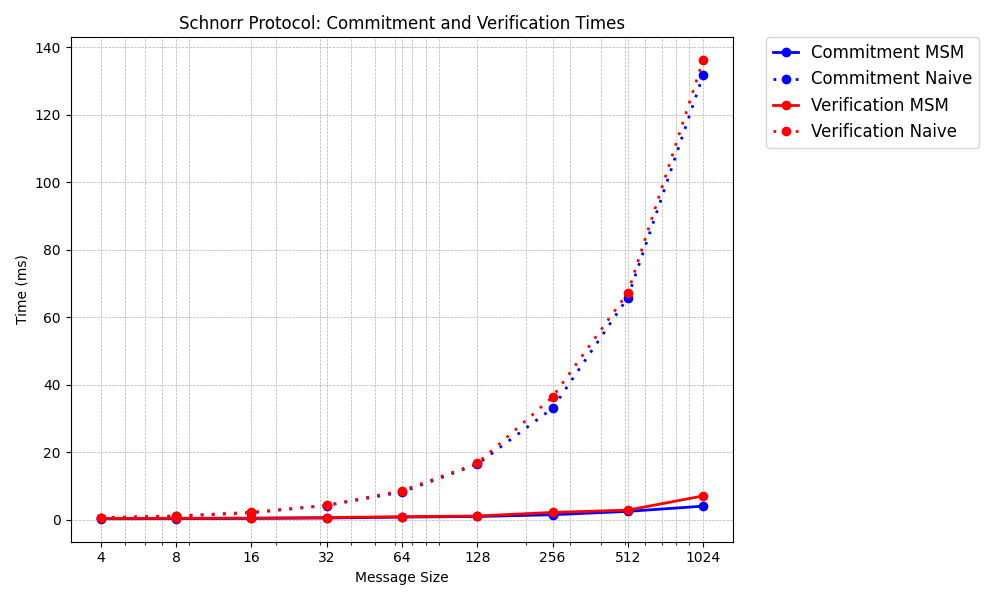
\includegraphics[width=0.75\linewidth]{schnorr_msm_no_msm.png}
    \caption{Schnorr Protocol - Practical Benchmarks with Multi-Scalar Multiplication}
    \label{fig:schnorr-benchmarks}
\end{figure}




\subsection{Pairing Protocols}

\begin{figure}
    \centering
    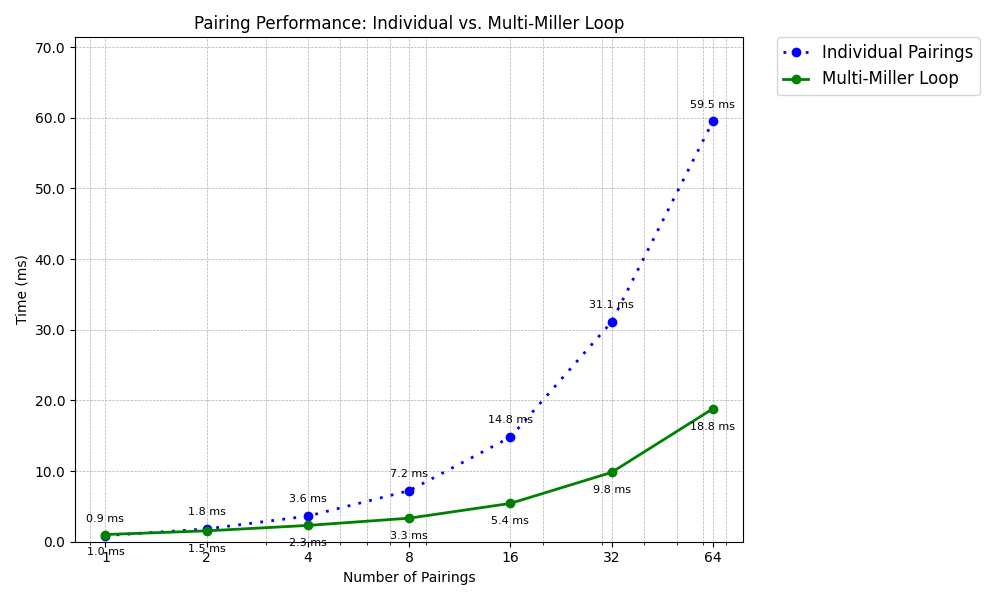
\includegraphics[width=0.75\linewidth]{pairing_comparison.png}
        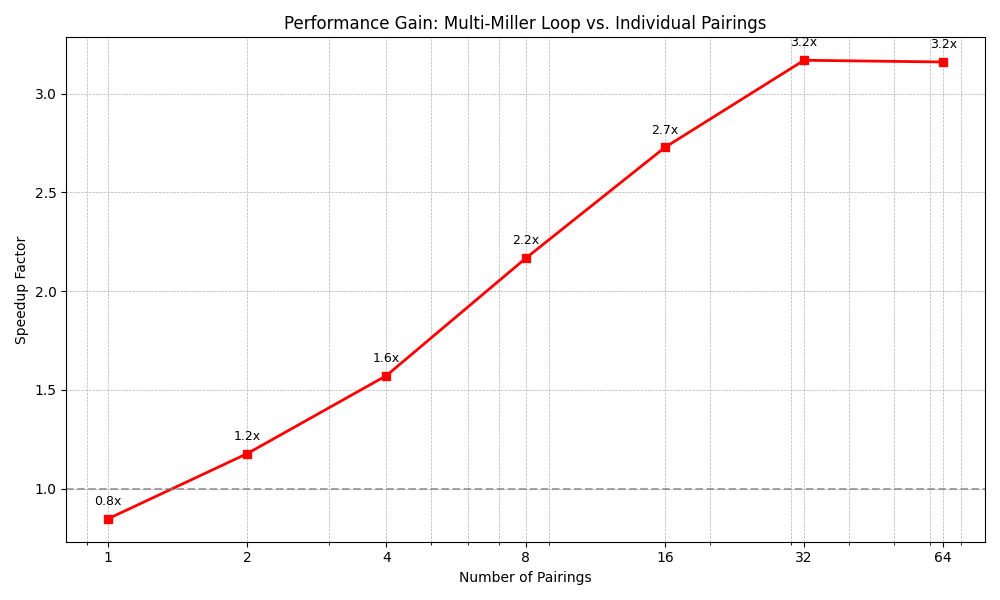
\includegraphics[width=0.75\linewidth]{pairing_comparison2.png}
    \caption{Elliptic Curve Pairings - Practical Benchmarks with Miller-Loop Intermediate Computation}
    \label{fig:enter-label}
\end{figure}



\ifnum\fullversion=0
  \bibliographystyle{splncs03}
 \else
   \bibliographystyle{alpha-short}
 \fi
 \bibliography{bib/abbrev3,bib/zotero, bib/custom}

\end{document}